\documentclass{simcenterdocumentation}
\usepackage[backend=biber]{biblatex}
%\usepackage{subfig}
\usepackage{subcaption}
\usepackage{multirow}
\usepackage{adjustbox}
\usepackage{cleveref}
\usepackage{longtable}

%% SETTING ENVIRONMENT FOR PYTHON CODE SNIPPETS %%%%%%%%%%%%%%%%%%%%%%%%%%%%%%% 
\usepackage[utf8]{inputenc}

\graphicspath{{../Common/}{.}} %Setting the graphicspath
\makeatletter % Search additional directories for inputs
\def\input@path{{../Common/}{.}}
%or: \def\input@path{{/path/to/folder/}{/path/to/other/folder/}}
\makeatother

%%%%%%%%%%%%%%%%%%%%%%%%%%%%%%%%%%%%%%%%%%%%%%%%%%%%%%%%%%%%%%%%%%%%%%%%%%%%%%% 

% To compile this file, run "latex/pdflatex codedoc", then "biber codedoc"
% (or "bibtex codedoc", if the output from latex asks for that instead),
% and then "latex/pdflatex codedoc" (without the quotes in each case).

% Double spacing, if you want it.  Do not use for the final copy. Can also specify
% draft as a document class option. This will generate double spacing and placeholders
% for title page and header images
%% \def\dsp{\def\baselinestretch{2.0}\large\normalsize}
%% \dsp

\bibliography{../Common/references}

\begin{document}

% Declarations for Front Matter
% Software title followed by optional second line
\title{uqFEM\\ \Large Uncertainty Quantification for Finite Element Modeling}
% Use superscripts to indicate author affiliations
\author{SimCenter Team}
%\author{Moe Howard$^{1,2}$ Larry Fine$^1$ Curly Howard$^2$}
\institutions{NHERI SimCenter, UC Berkeley}
\softwarename{uqFEM}
\softwareversion{1.2}
\softwarepage{https://simcenter.designsafe-ci.org/research-tools/uqfem-application/}

%%% DON'T MESS WITH THESE SETTINGS %%%%%%%%%%%%%%%%%%%%%%%%%%%%%%%%
\hypersetup{pageanchor=false}
\maketitle
\copyrightpage
\acknowledgments

\hypersetup{pageanchor=true}
\begin{frontmatter}

\pagestyle{plain}
{
  \renewcommand{\thispagestyle}[1]{}
  \tableofcontents
  \clearpage
  \listoffigures
  \clearpage
  \listoftables
}

\end{frontmatter}
\pagestyle{somewhatsimple}
%%%%%%%%%%%%%%%%%%%%%%%%%%%%%%%%%%%%%%%%%%%%%%%%%%%%%%%%%%%%%%%%%%%
% Create separate tex files for each chapter and provide them as inputs

%\chapter{About}
%\label{chap:about}
%The intended audience for this tool is researchers and practitioners
interested in predicting the response of a structure to earthquake
events.\\

This open-source research application, the source code of which is
available at
the \href{https://github.com/NHERI-SimCenter/EE-UQ}{\texttt{\getsoftwarename{}}
Github page}, provides an application that can be used to predict the
response of a building subjected to earthquake events. The application
is focused on quantifying the uncertainties in the predicted response,
given the that the properties of the buildings and the earthquake
events are not known exactly, and that both the simulation software
and the user make simplifying assumptions in the numerical modeling of
that structure. In this application, the user is required to
characterize the uncertainties in the input. The application will,
after utilizing the users selected sampling method, provide
information that characterizes the uncertainties in the computed
response measures. As the computations to make these determinations
can be prohibitively expensive to perform on a user's local computer,
the user has the option to perform the computations remotely on the
Stampede2 supercomputer. Stampede2 is located at the Texas Advanced
Computing Center (TACC) and made available to the user through NHERI
DesignSafe, the cyberinfrastructure provider for the distributed NSF
funded Natural Hazards in Engineering Research Infrastructure (NHERI)
facility.\\

Whether running locally or remotely, the computations are performed,
as will be discussed in \Cref{chap:theory}, in a workflow
application. That is, the numerical simulations are actually performed
by a number of different applications. The \texttt{\getsoftwarename{}} backend software runs
these different applications for the user, taking the outputs from
some programs and providing them as inputs to others. The design of
the \texttt{\getsoftwarename{}} application is such that researchers are able to modify the
backend application to utilize their own application in the workflow
computations. This will ensure researchers are not limited to using
the default applications we provide and will be enthused to provide
their own applications for others to use. \\

This document covers Version \getsoftwareversion{} of the tool. Users are
encouraged to comment on what additional features and capabilities
they would like to see in this application. These requests and
feedback can be submitted through an anonymous \insertsurveylink{user
survey}; we greatly appreciate any input you have. If there are
features you want, chances are many of your colleagues also would
benefit from them. Users are encouraged to review
\Cref{chap:requirements} to see what features are planned for this
application.


%\chapter{Installation Instructions}
%\label{chap:installation}
%All SimCenter applications are available at
the \href{https://simcenter.designsafe-ci.org/research-tools/overview/}{SimCenter
website} under \emph{Research Tools}. The following sections outline
the steps necessary to download and install the \texttt{\getsoftwarename{}}
application. The SimCenter applications do require that you install a
number of other applications that are needed to run the workflows on
your local machine as well as at DesignSafe. \\


%===============================================================================
\section{Download the Application}
%===============================================================================

% \subsection{Download the Application Files}

To download the \texttt{\getsoftwarename{}} application navigate to
the \getsoftwarepage{\texttt{\getsoftwarename{}} page} and click on
the \emph{Download App \& User Manual} link on the right side of the
page. As shown in \Cref{fig:app_choose_file}, this will bring you to another page which contains a list of downloadable files and directories.

\softwareSwitch{PBE}{
\begin{figure}[!htbp]
  \centering {
    \includegraphics[width=0.95\textwidth]
OA    {installation/figures/pbeDownload.png} }
  \caption{Download Application}
  \label{fig:app_choose_file}
\end{figure}
}{}

\softwareSwitch{EE-UQ}{
\begin{figure}[!htbp]
  \centering {
    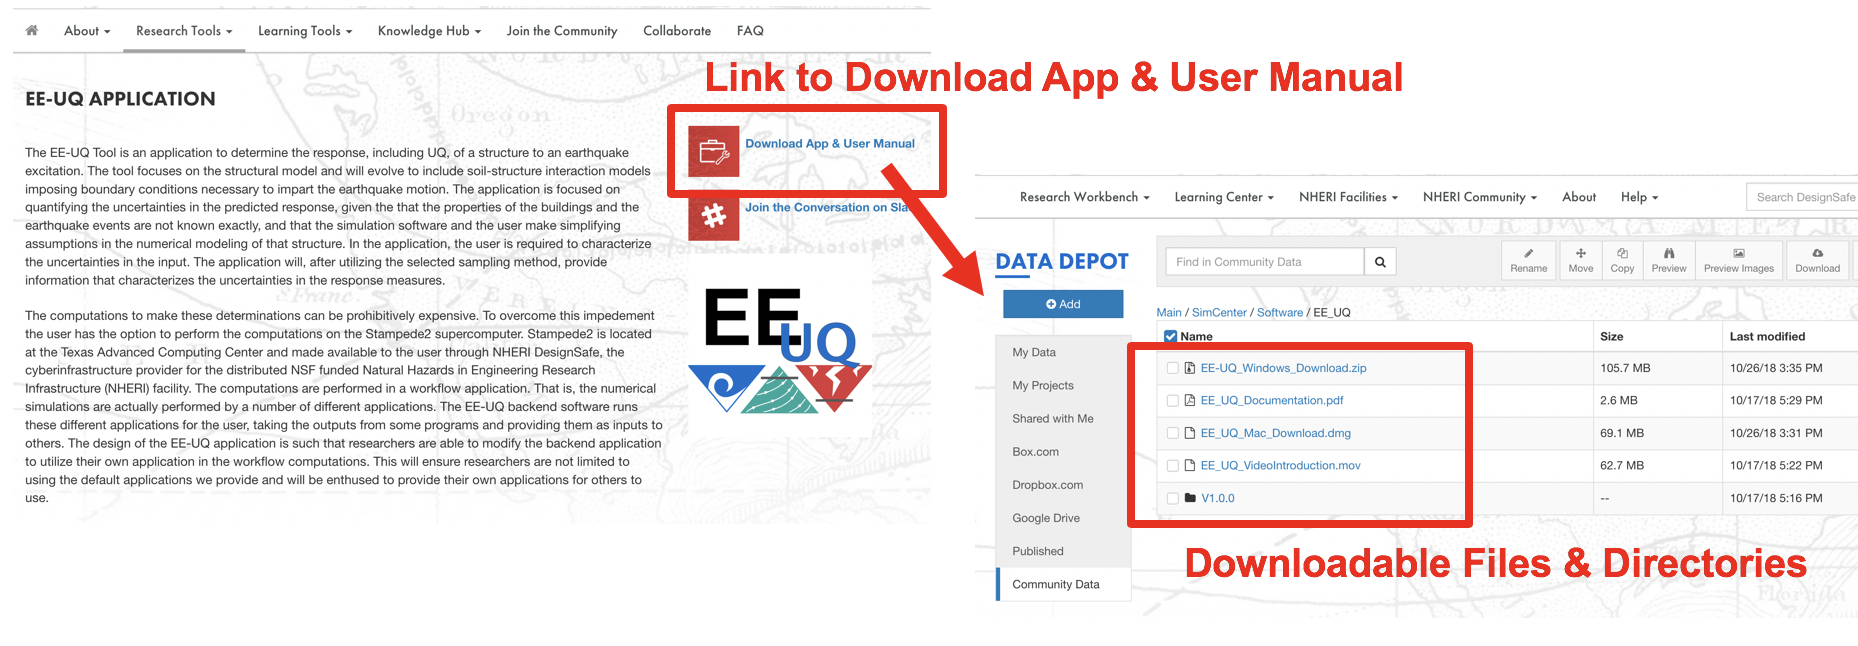
\includegraphics[width=0.95\textwidth]
    {installation/figures/eeDownload.png} }
  \caption{Download Application}
  \label{fig:app_choose_file}
\end{figure}
}{}

\softwareSwitch{WE-UQ}{
\begin{figure}[!htbp]
  \centering {
    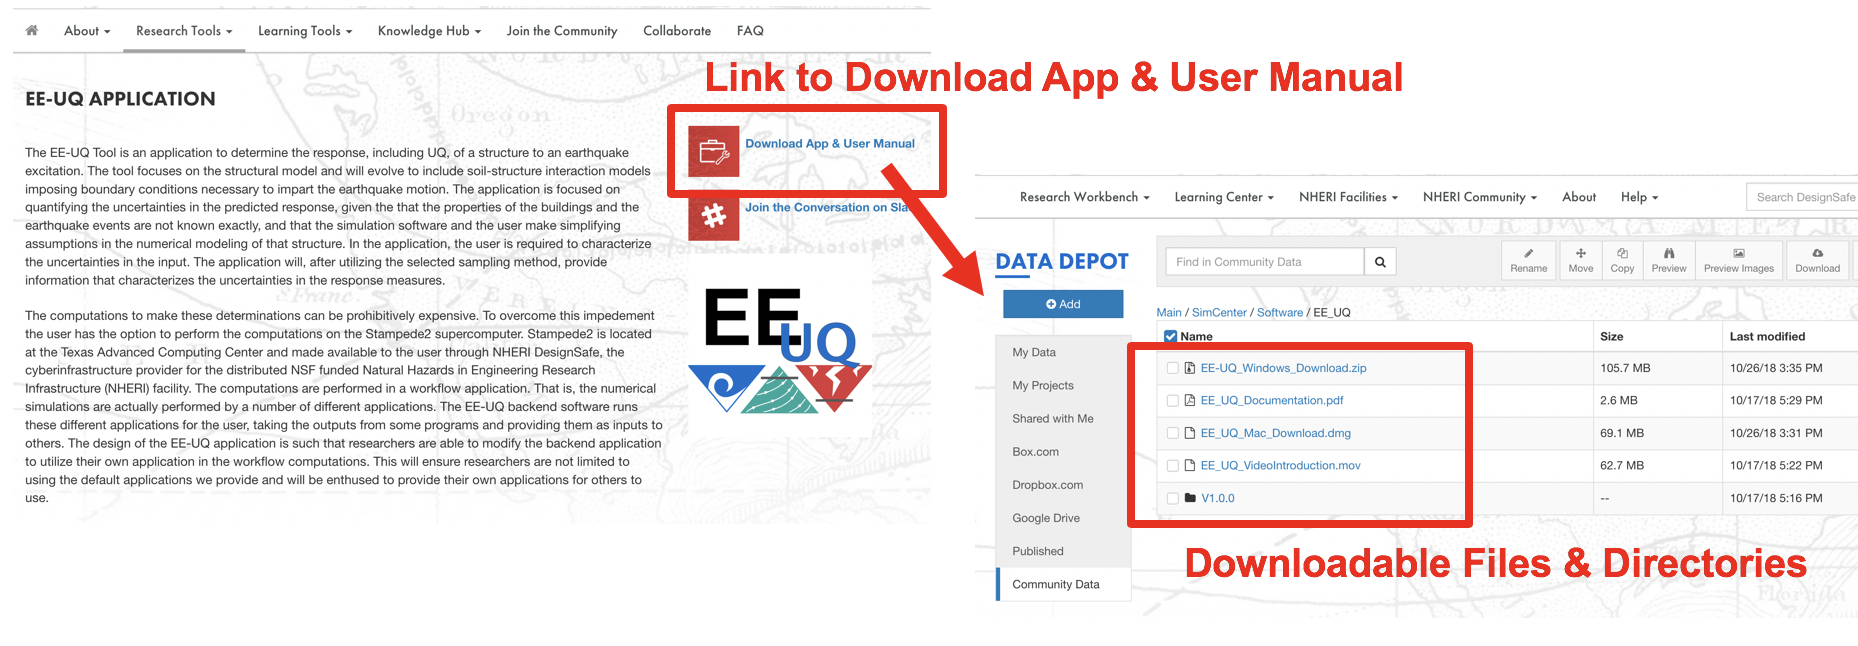
\includegraphics[width=0.95\textwidth]
    {installation/figures/eeDownload.png} }
  \caption{Download Application}
  \label{fig:app_choose_file}
\end{figure}
}{}


There are at least four files available for download from this page: 
\begin{enumerate}
    \item The PDF file is the User Manual that you are reading now.
    \item The MOV file is an video that provides an introduction to the usage of the application.
    \item The ZIP file is an archive that contains the application files for a Windows operating system.
    \item The DMG file is an archive that contains the application files for a Mac OS X operating system.
\end{enumerate}

To download the \texttt{\getsoftwarename{}} application click on the link for
the appropriate file for your operating system and then click on the
Download button at bottom right corner of the ensuing pop-up window. 
Unpackage the application from the downloaded
file and place it in a location on your filesystem. On Windows, we
recommend that you create a \texttt{C:/SimCenter/\getsoftwarename{}}
directory and extract the contents of the \texttt{ZIP} archive
there. It is also recommended to run the included installer for Visual C/C++ runtime library(vc\_redist.x64.exe). 
If you use a Mac we recommend you copy the application to either your
Documents folder or your Desktop folder. You are free to place the
applications anywhere you wish, you will need to make the
appropriate adjustments with the following instructions if you do so. \\

Now test that the application starts. To do this navigate to
the location where you placed the application and open it. You should
see the user interface (UI) shown in \Cref{fig:app_UI} after
starting the application. Now Quit the application. Additional steps are required before 
computations can be performed.\\

\softwareSwitch{PBE}{
\begin{figure}[!htbp]
  \centering {
    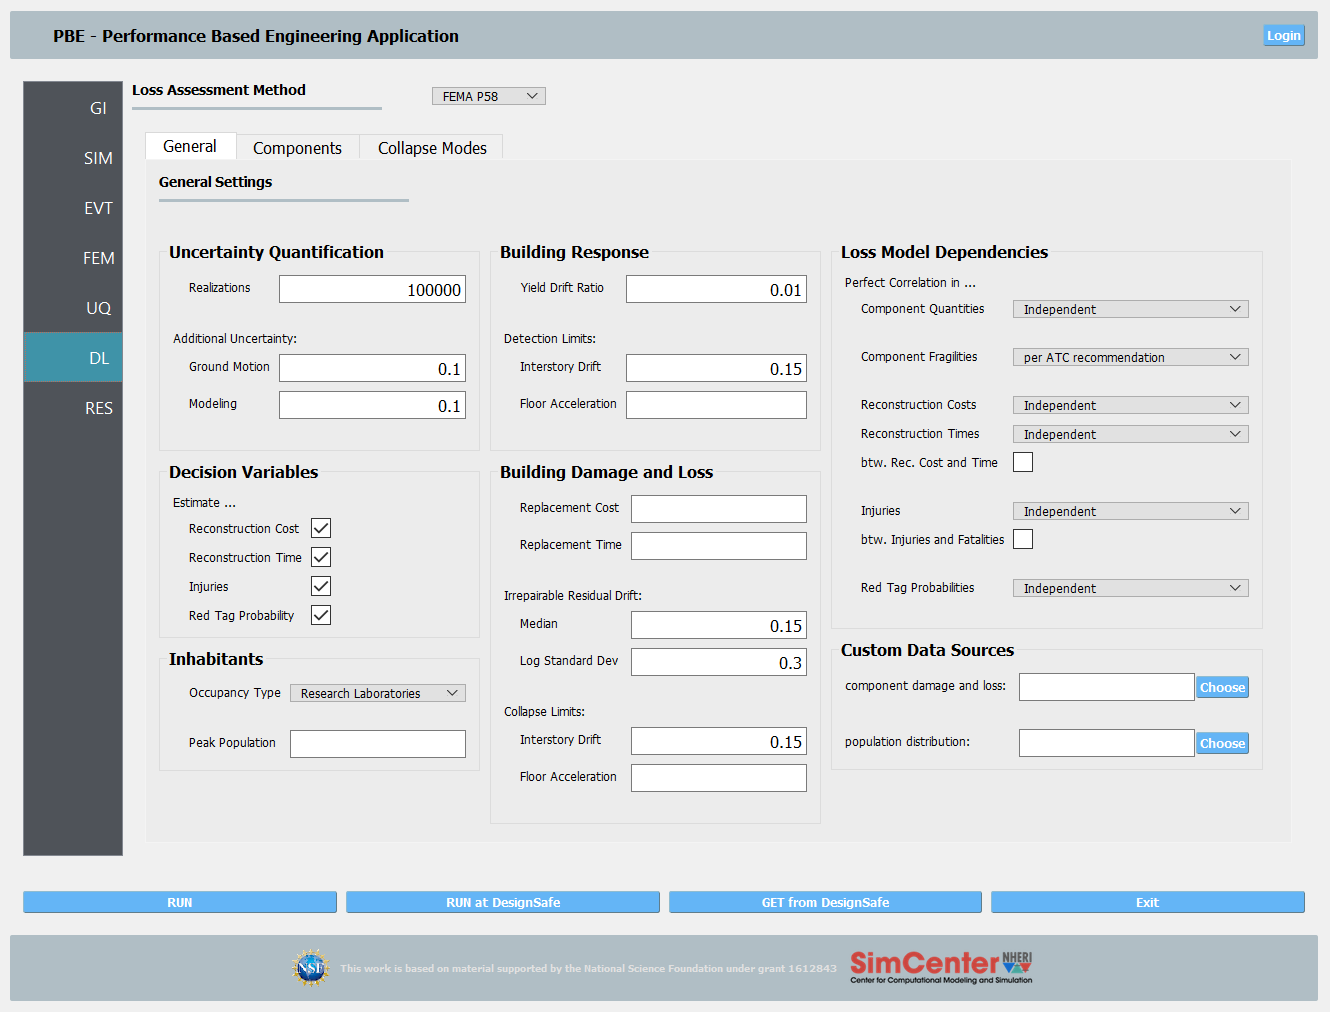
\includegraphics[width=0.95\textwidth]
    {installation/figures/PBE.png} }
  \caption{PBE Application on Startup}
  \label{fig:app_UI}
\end{figure}
}{}

\softwareSwitch{EE-UQ}{
\begin{figure}[!htbp]
  \centering {
    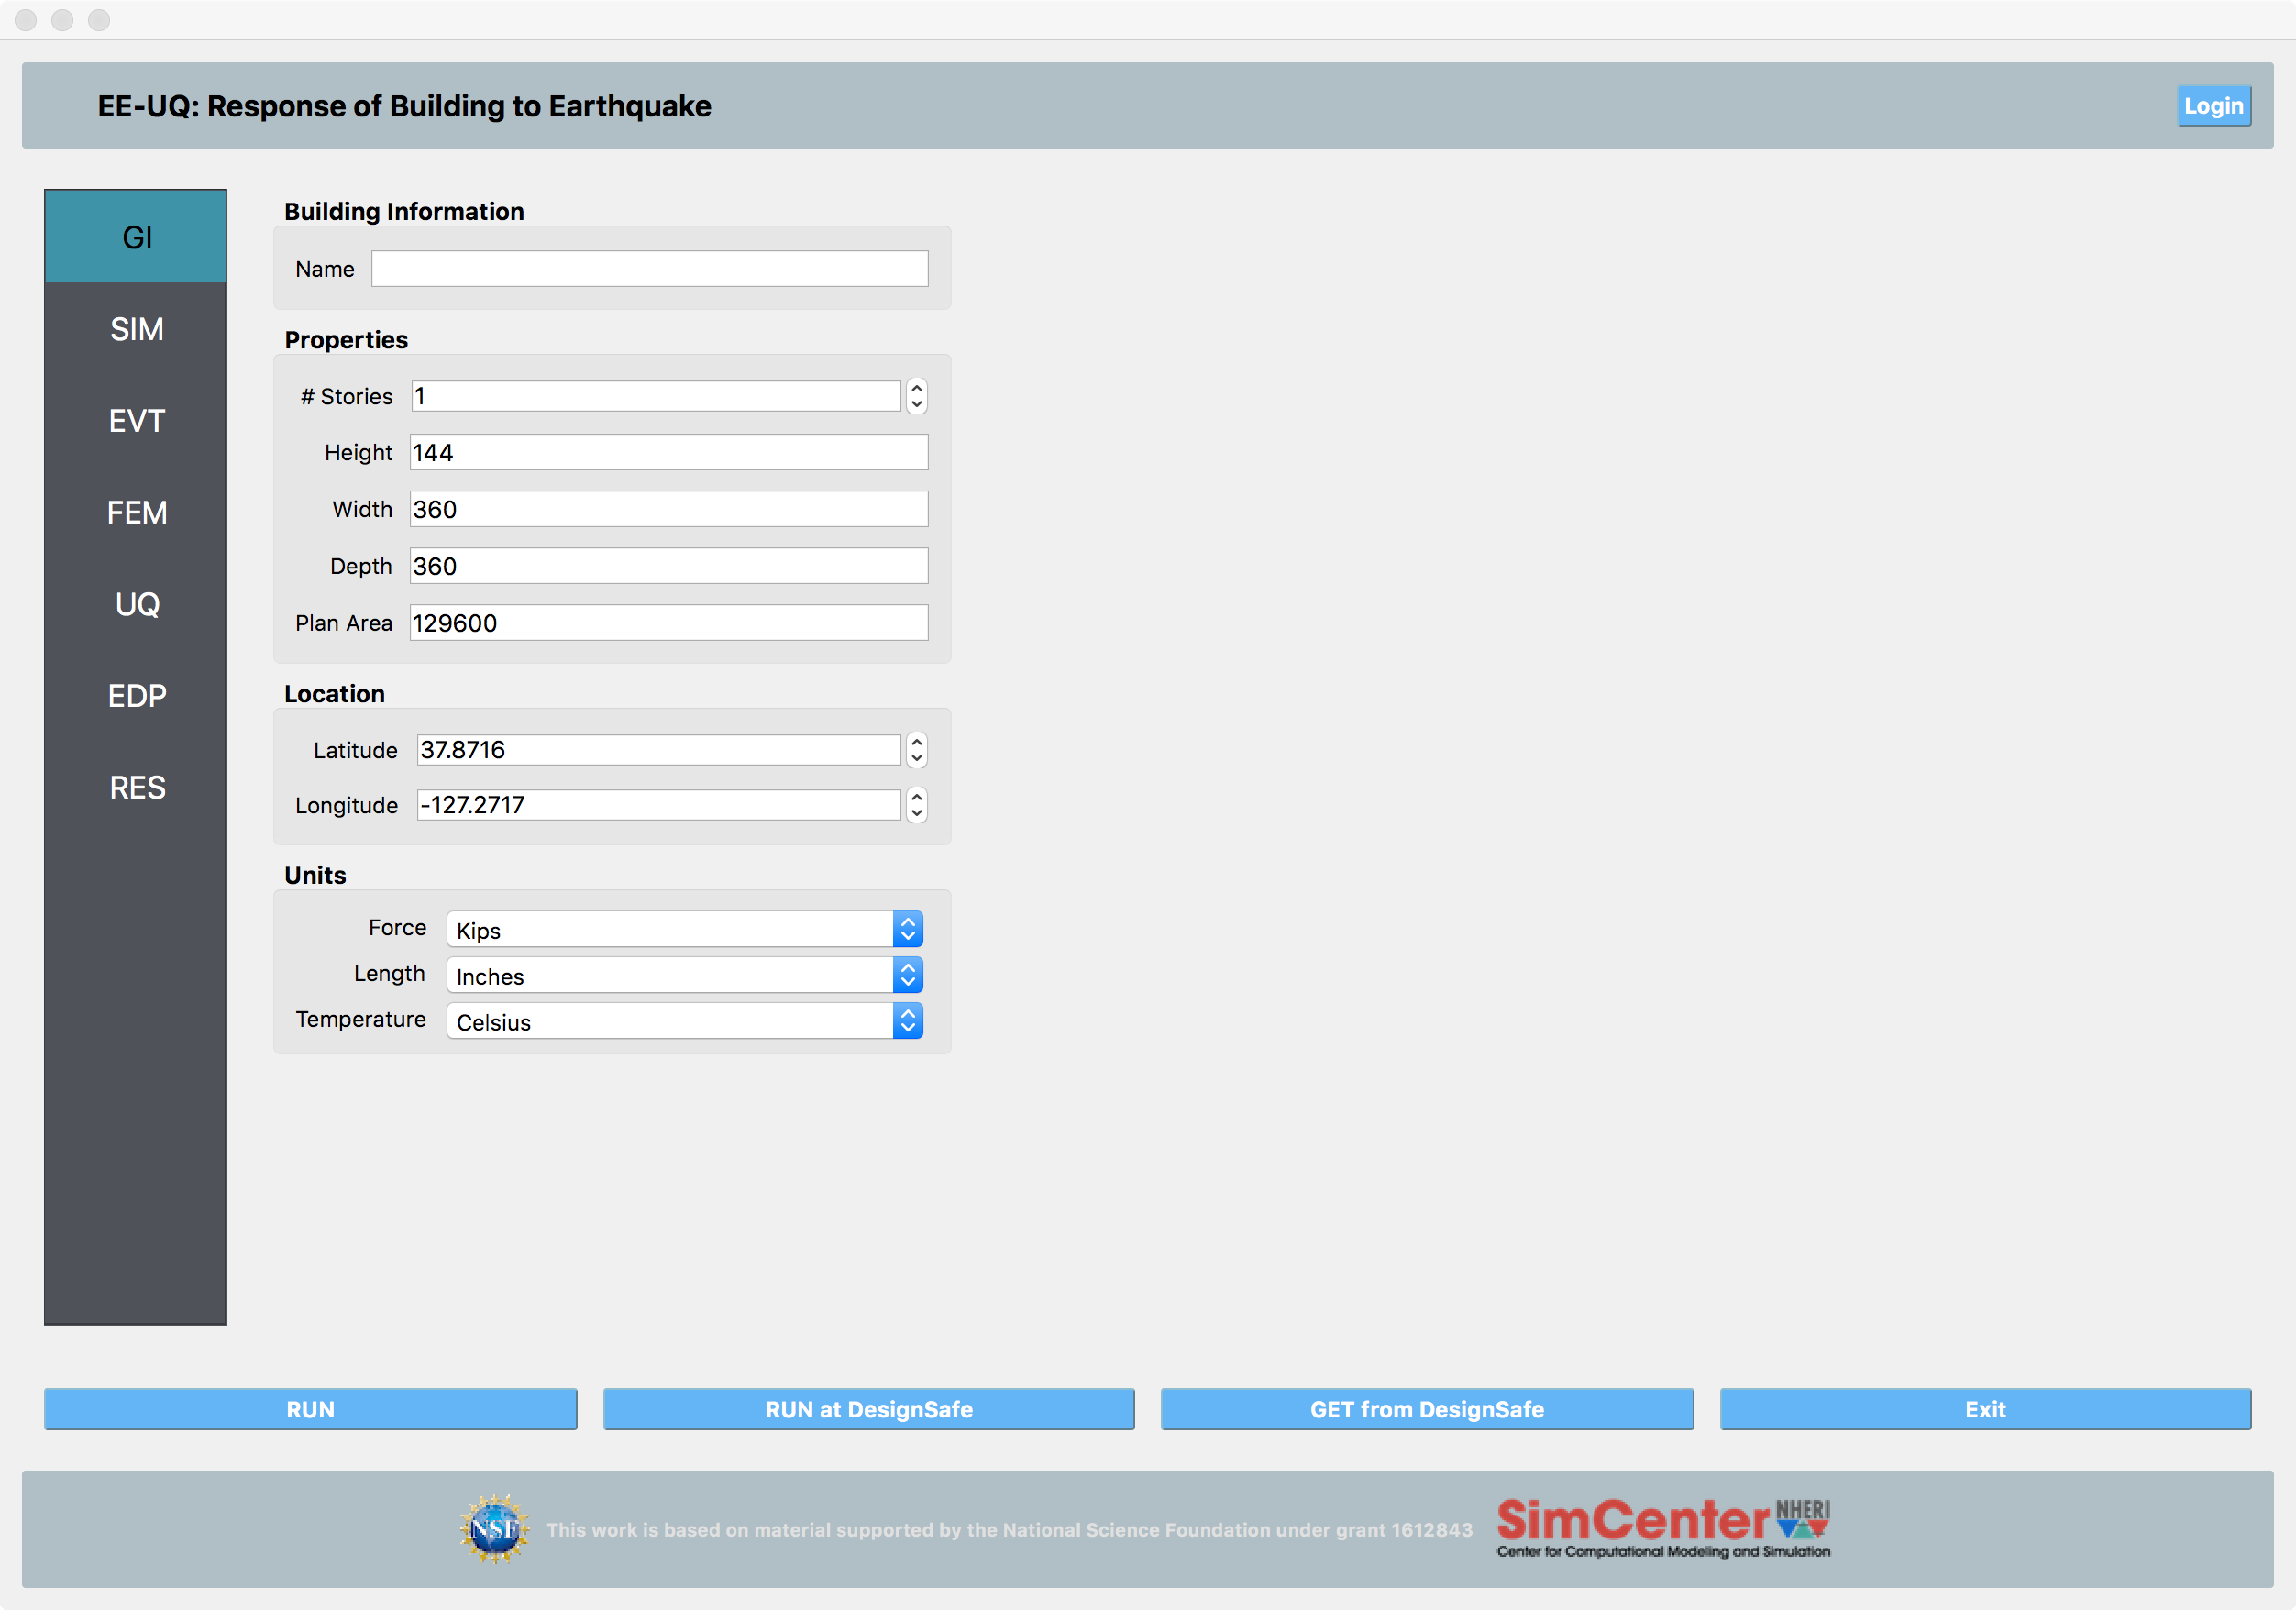
\includegraphics[width=0.95\textwidth]
    {installation/figures/EE-UQ.png} }
  \caption{EE-UQ Application on Startup}
  \label{fig:app_UI}
\end{figure}
}{}

\softwareSwitch{WE-UQ}{
\begin{figure}[!htbp]
  \centering {
    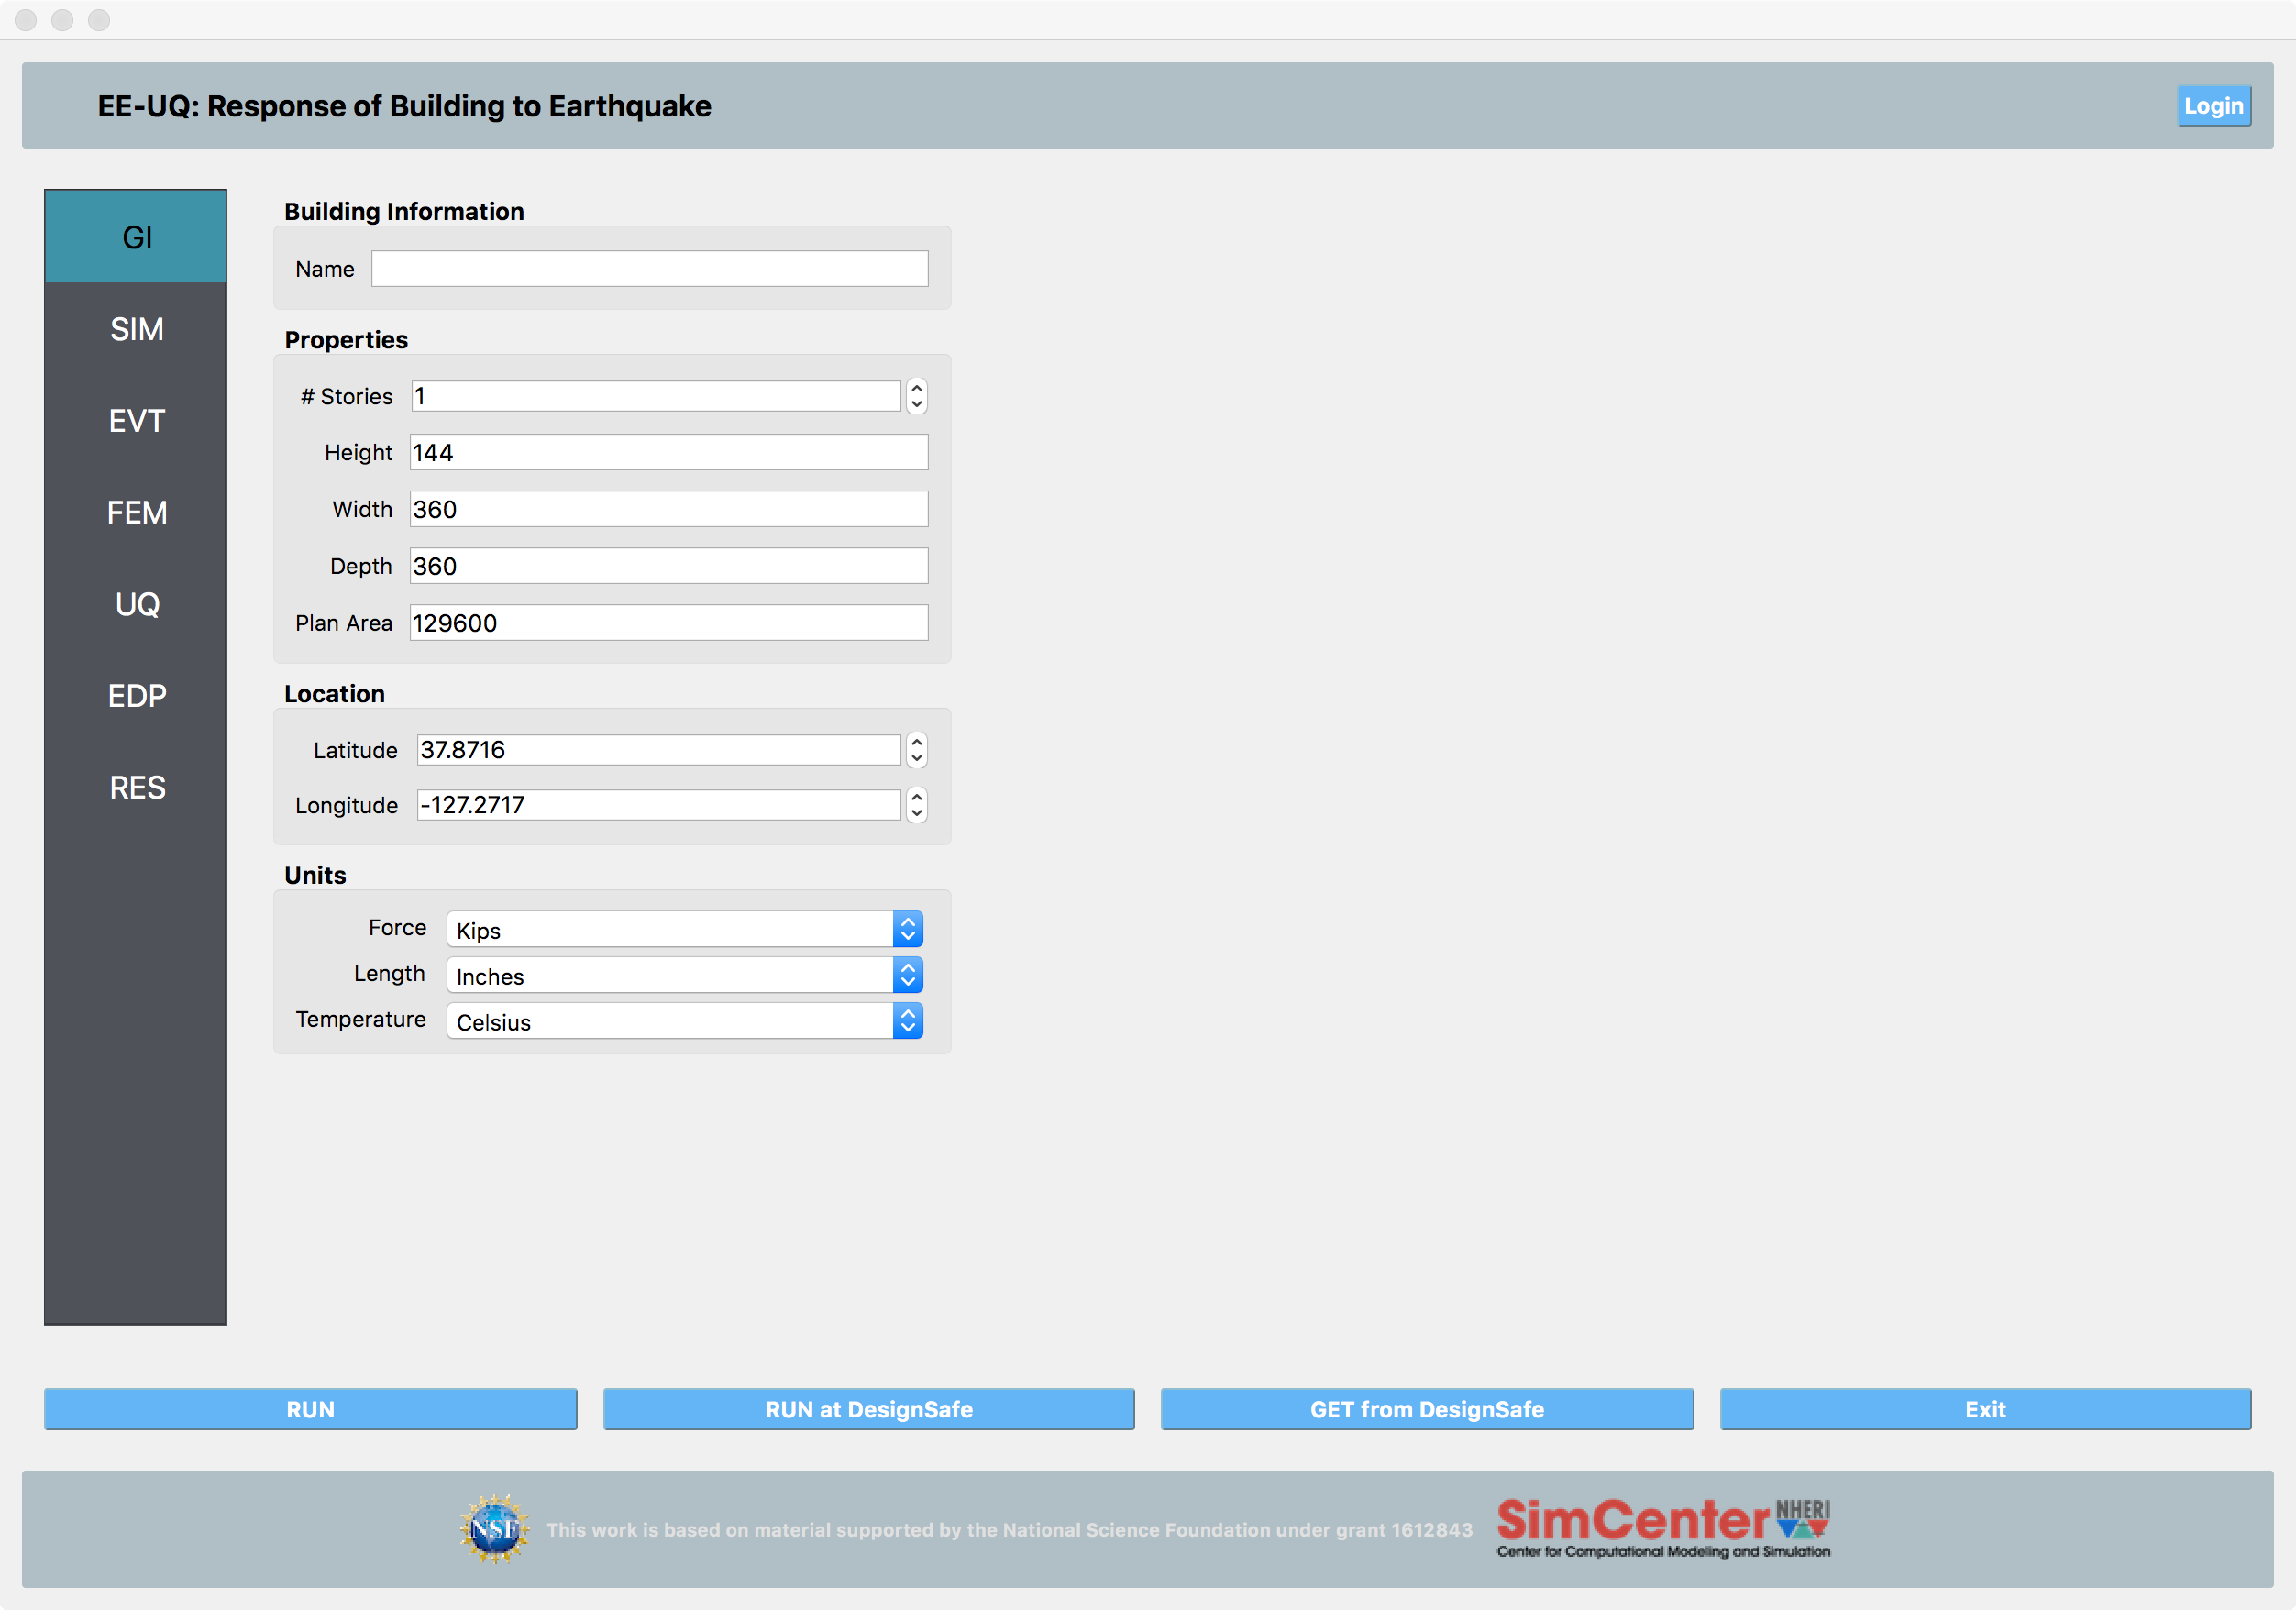
\includegraphics[width=0.95\textwidth]
    {installation/figures/EE-UQ.png} }
  \caption{WE-UQ Application on Startup}
  \label{fig:app_UI}
\end{figure}
}{}


\begin{enumerate}
\item The SimCenter is not recognized as either a Windows or an Apple vendor. Our applications are not recognized by the operating system as being signed. Consequently, you may receive a warning message when you start the \texttt{\getsoftwarename{}} application for the first time.
\item  On a Mac you will need to right click on the .dmg file to open it. The UI will not start correctly while in the DMG file, you need to open the .dmg file and then copy the \texttt{\getsoftwarename{}} application to your Documents or Desktop folder. You can then move the .dmg file to the trash or eject it after this has been done.
\item  The \texttt{\getsoftwarename{}} application requires additional software outlined in next subsections to work properly. Even of the software starts correctly, it will not run correctly until this software, outlined in the next section, is installed correctly.
\end{enumerate}


%===============================================================================
\section{Set up Python}
%===============================================================================

The SimCenter workflow applications are managed by Python
scripts. These are required to prepare the input data for running
analyses either remotely on DesignSafe or locally. As a consequence the user must have Python
installed on their machine and have the appropriate environment
variables set so that the UI can run these applications.

\subsection{Install Python}

If you have not yet installed Python, we recommend
installing \href{http://www.anaconda.com/distribution/#download-section}{Anaconda}. Anaconda
provides all the important scientific packages in a single convenient
install. We recommend installing the 64-Bit version based on Python
3.5 or newer.

Note: If you already have a Python installation that is Python 2.7 or
newer, you do not have to install Anaconda to work with SimCenter
applications as you may also use another Python distribution.
If you do please make sure that you install the following packages: 
\texttt{numpy}, \texttt{scipy}, and \texttt{pandas}.

\subsection{Test Python}
%===============================================================================

Test if the python environment is set up properly by
executing \texttt{python} in a terminal window. After Python starts,
test if the packages are installed by executing \texttt{import
numpy}, \texttt{import scipy}, and \texttt{import pandas}. You will
receive an error message if a pacakage is missing. If no error
appears, the terminal should look similar
to \Cref{fig:python_test}. Exit Python by executing
the \texttt{exit()} command.

\begin{figure}[!htbp]
  \centering {
    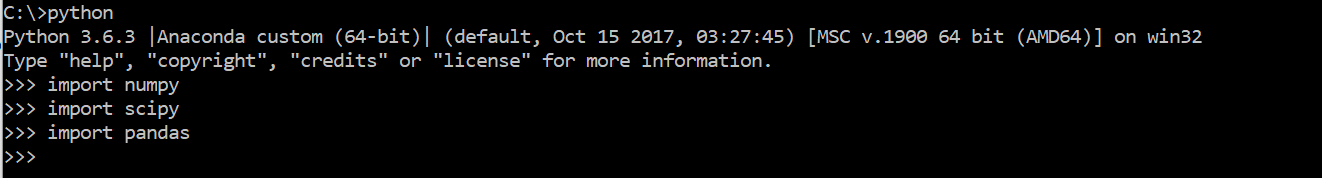
\includegraphics[width=0.8\textwidth]
    {installation/figures/python_test.png} }
  \caption{Testing the Python environment.}
  \label{fig:python_test}
\end{figure}

%===============================================================================
\section{Set up for Running Workflows Locally}\label{setup}
%===============================================================================

To run the workflows locally, the backend python application needs
publicly available software to also be installed on your
machine. These software applications need to be installed and
configured on your operating system. If you do not plan to run the
workflows locally, you will not need these applications.

\subsection{Install \texttt{OpenSees}}
%===============================================================================

\href{http://opensees.berkeley.edu}{\texttt{OpenSees}} is an open-source finite element application publicly available for download from its \href{http://opensees.berkeley.edu/OpenSees/user/download.php}{download page}. \texttt{OpenSees} installation requires the user install both \texttt{OpenSees} and \texttt{Tcl}.  If you have never downloaded \texttt{OpenSees} before, you will need to register your e-mail to gain access. After registration, you can proceed to the download page by entering your email address and clicking the Submit button. The Windows and Mac downloads are in different locations on the download page, with the appropriate Tcl installer beside the \texttt{OpenSees} link; see \Cref{fig:openseesDownload}

\begin{figure}[!htbp]
  \centering {
    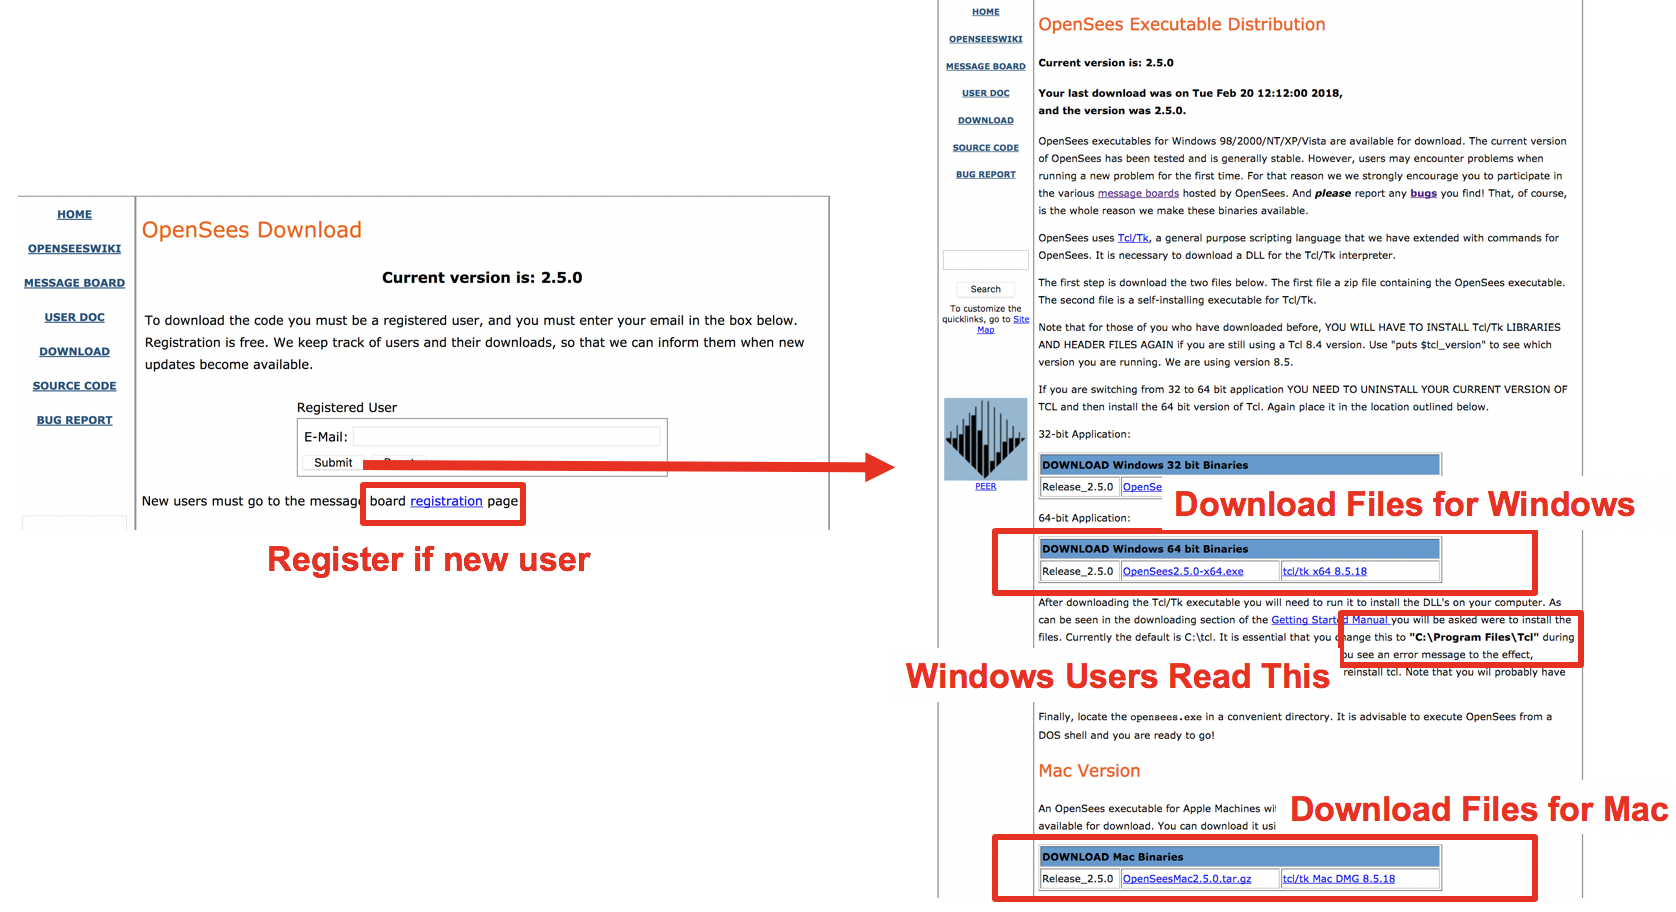
\includegraphics[width=\textwidth]
    {installation/figures/openseesDownload.png} }
  \caption{Downloading OpenSees}
  \label{fig:openseesDownload}
\end{figure}

Follow the instructions on the download page to install \texttt{Tcl}
(\Cref{fig:openseesDownload}). On Windows, you must select the Custom option for installton and you must specify
the installtion directory as \texttt{C:\textbackslash Program Files\textbackslash Tcl}, 
which is not the default. \\

After \texttt{Tcl} is installed, we recommend you put \texttt{OpenSees} in
the \texttt{C:/SimCenter/OpenSees} folder on Windows and in
a \texttt{/usr/local/OpenSees} directory on the Mac (If you use finder
on Mac to do navigation, use command-shift-G in Finder and specify
/usr/local as the folder to go to. Create a new folder \texttt{OpenSees}
and copy the \texttt{OpenSees} application to this folder).\\


Now you need to add the \texttt{OpenSees} folder to the
system \texttt{PATH} environment variable to allow the SimCenter
workflow applications to find the \texttt{OpenSees} executable on your
computer. The steps to do this depend on your operating system:

\begin{enumerate}
\item Windows: To add a folder to the \texttt{PATH} on Windows (\Cref{fig:add_env_path}):

\begin{figure}[!htbp]
  \centering {
    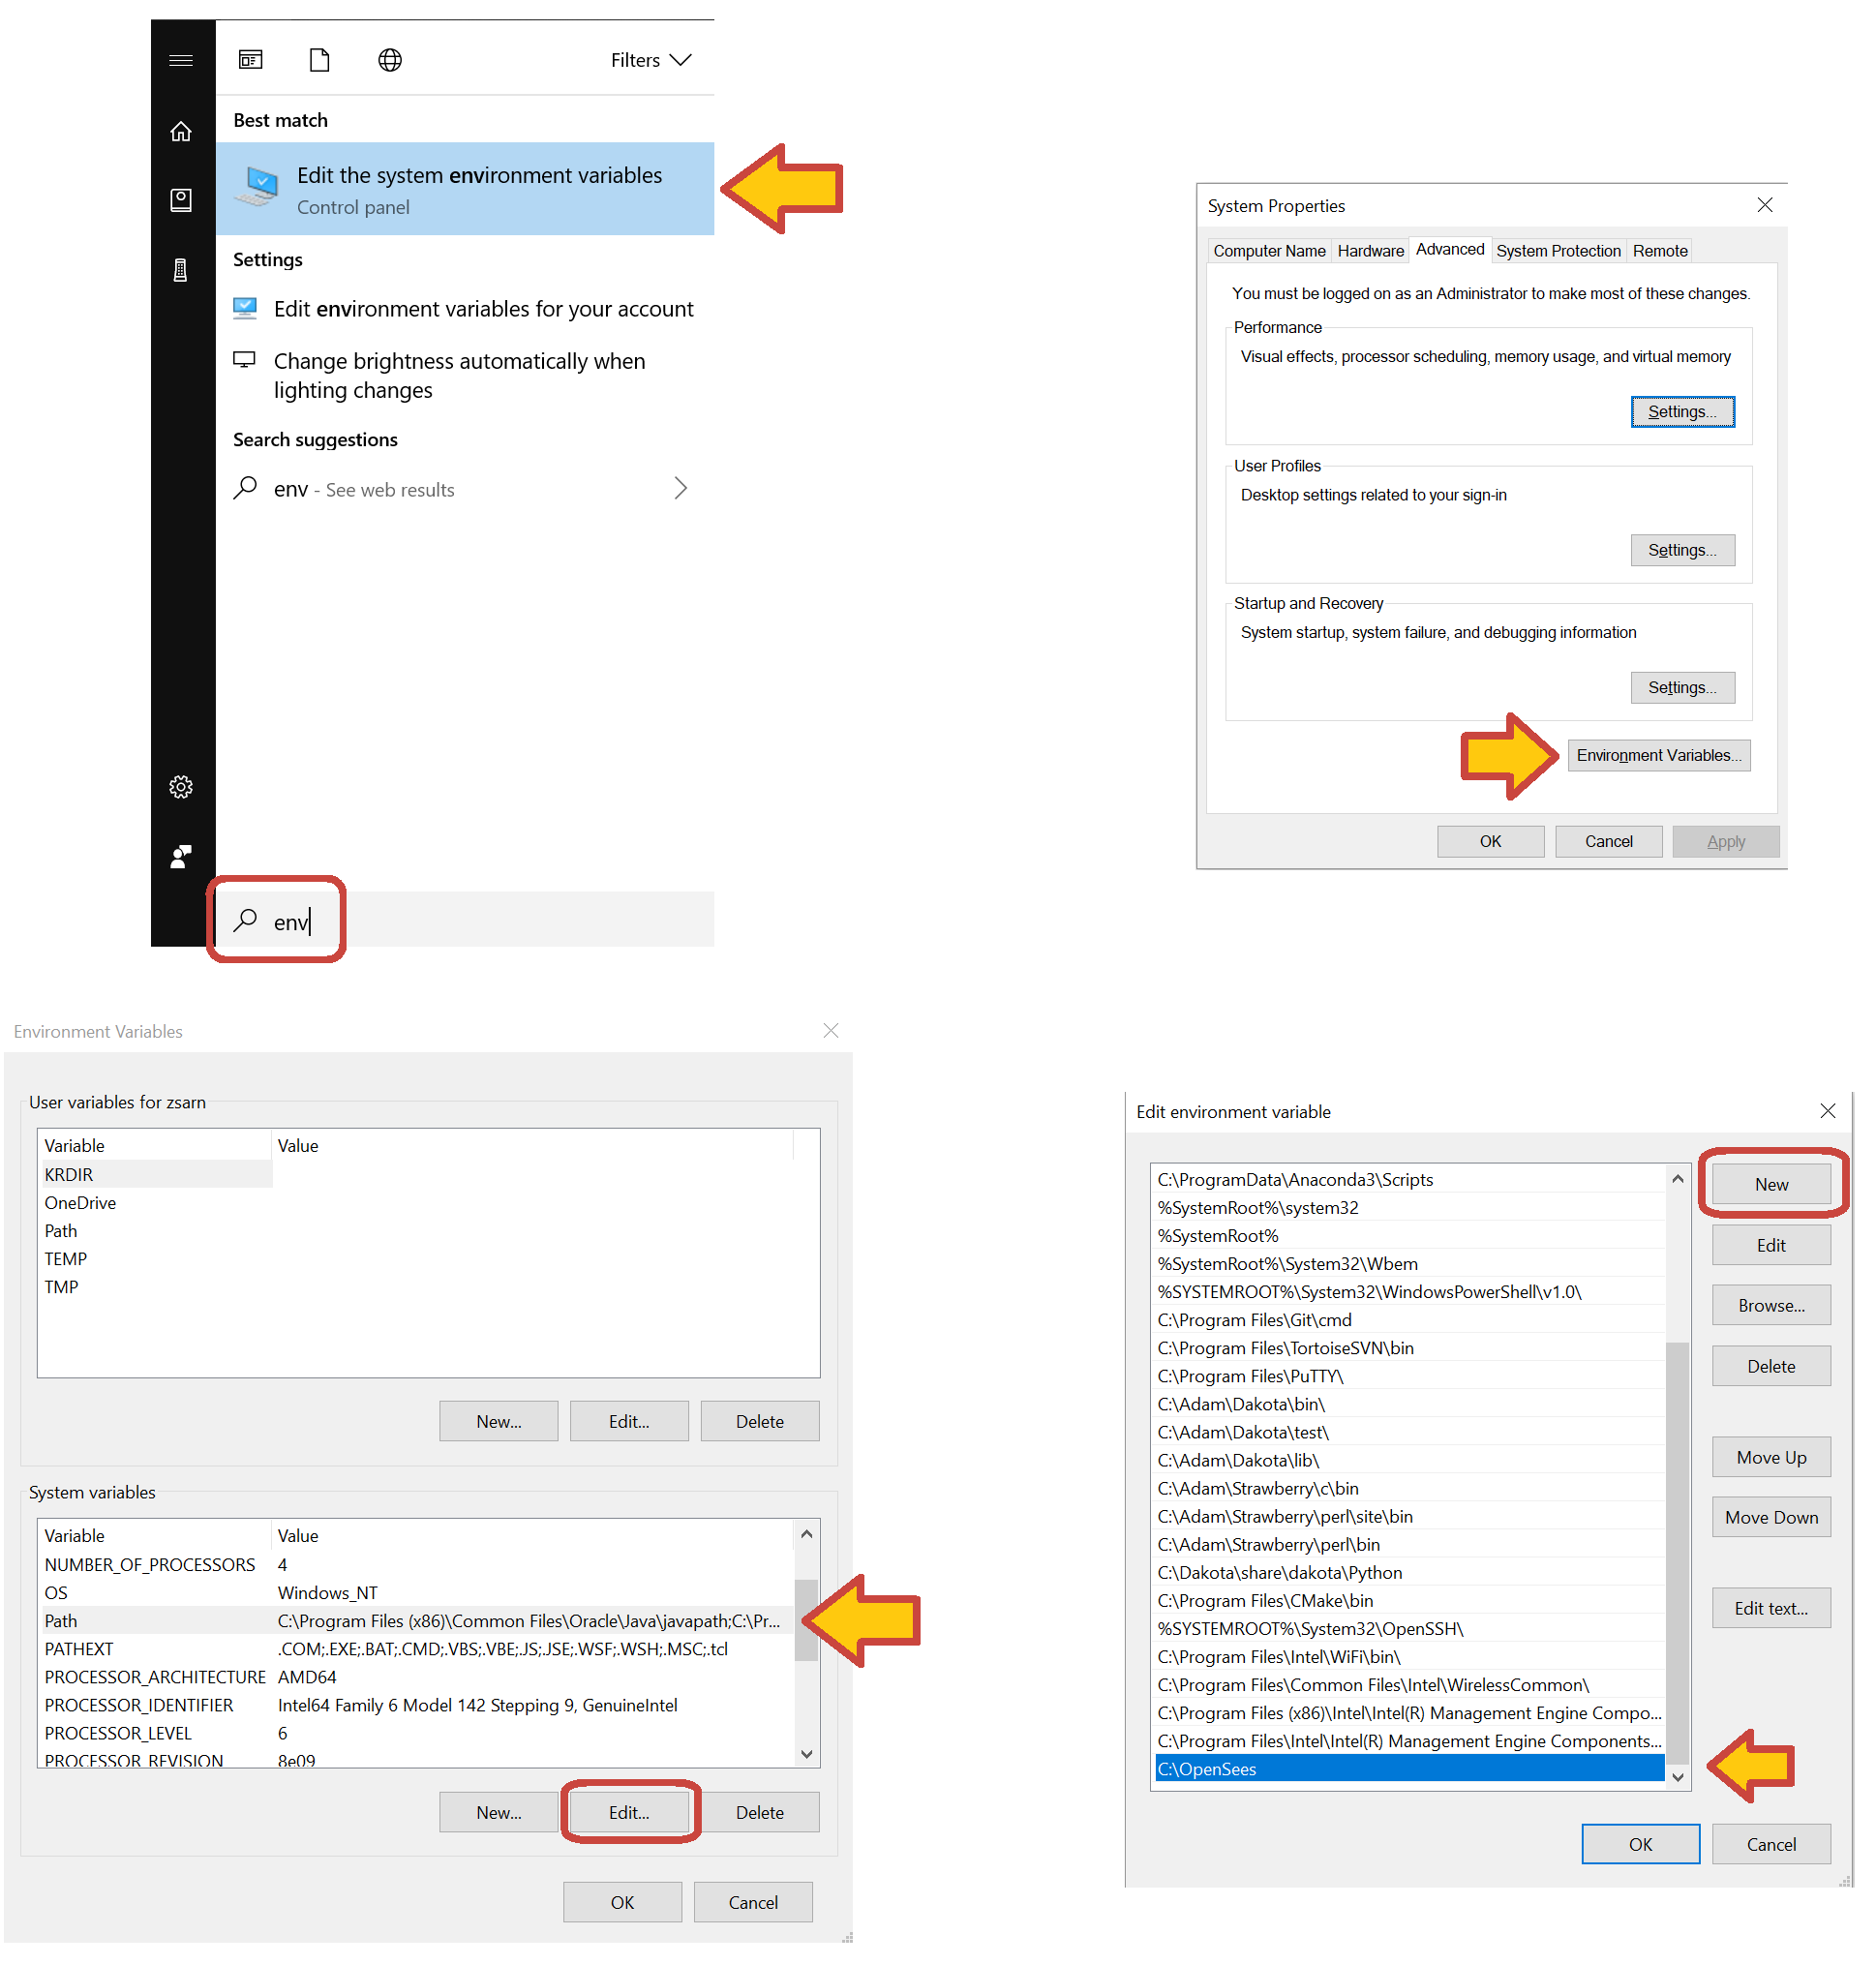
\includegraphics[width=0.8\textwidth]
    {installation/figures/add_env_path.png} }
  \caption{Adding OpenSees to the PATH environment variable on Windows}
  \label{fig:add_env_path}
\end{figure}


\begin{enumerate}
    \item open \emph{Start}, type \emph{env}, and choose \emph{Edit the system environment variables};
    \item click on the \emph{Environment variables...} button in the dialog window;
    \item find the \texttt{Path} under \emph{System Variables} in the \emph{Variable} column;
    \item click \emph{New} and type in the path to your \texttt{OpenSees.exe} (this will be \texttt{C:\textbackslash SimCenter\textbackslash OpenSees} if you put the executable at the recommended location - pay attention to using backslashes here!);
    \item click \emph{OK} in every dialog to close them and save your changes.
\end{enumerate}

\item MacOS: To add the /usr/local/OpenSees folder to the \texttt{PATH} variable:


\begin{enumerate}
    \item open a Terminal;
    \item execute \texttt{sudo nano /etc/paths} and enter your password
    \item add the path to the \texttt{OpenSees} executable to the end of the list (this will be \texttt{/usr/local/OpenSees} if you put the executable at the recommended location);
    \item quit by hitting \texttt{Ctrl+X} and then \texttt{Y} when asked if you want to save modifications.
\end{enumerate}

\begin{figure}[!htbp]
  \centering {
     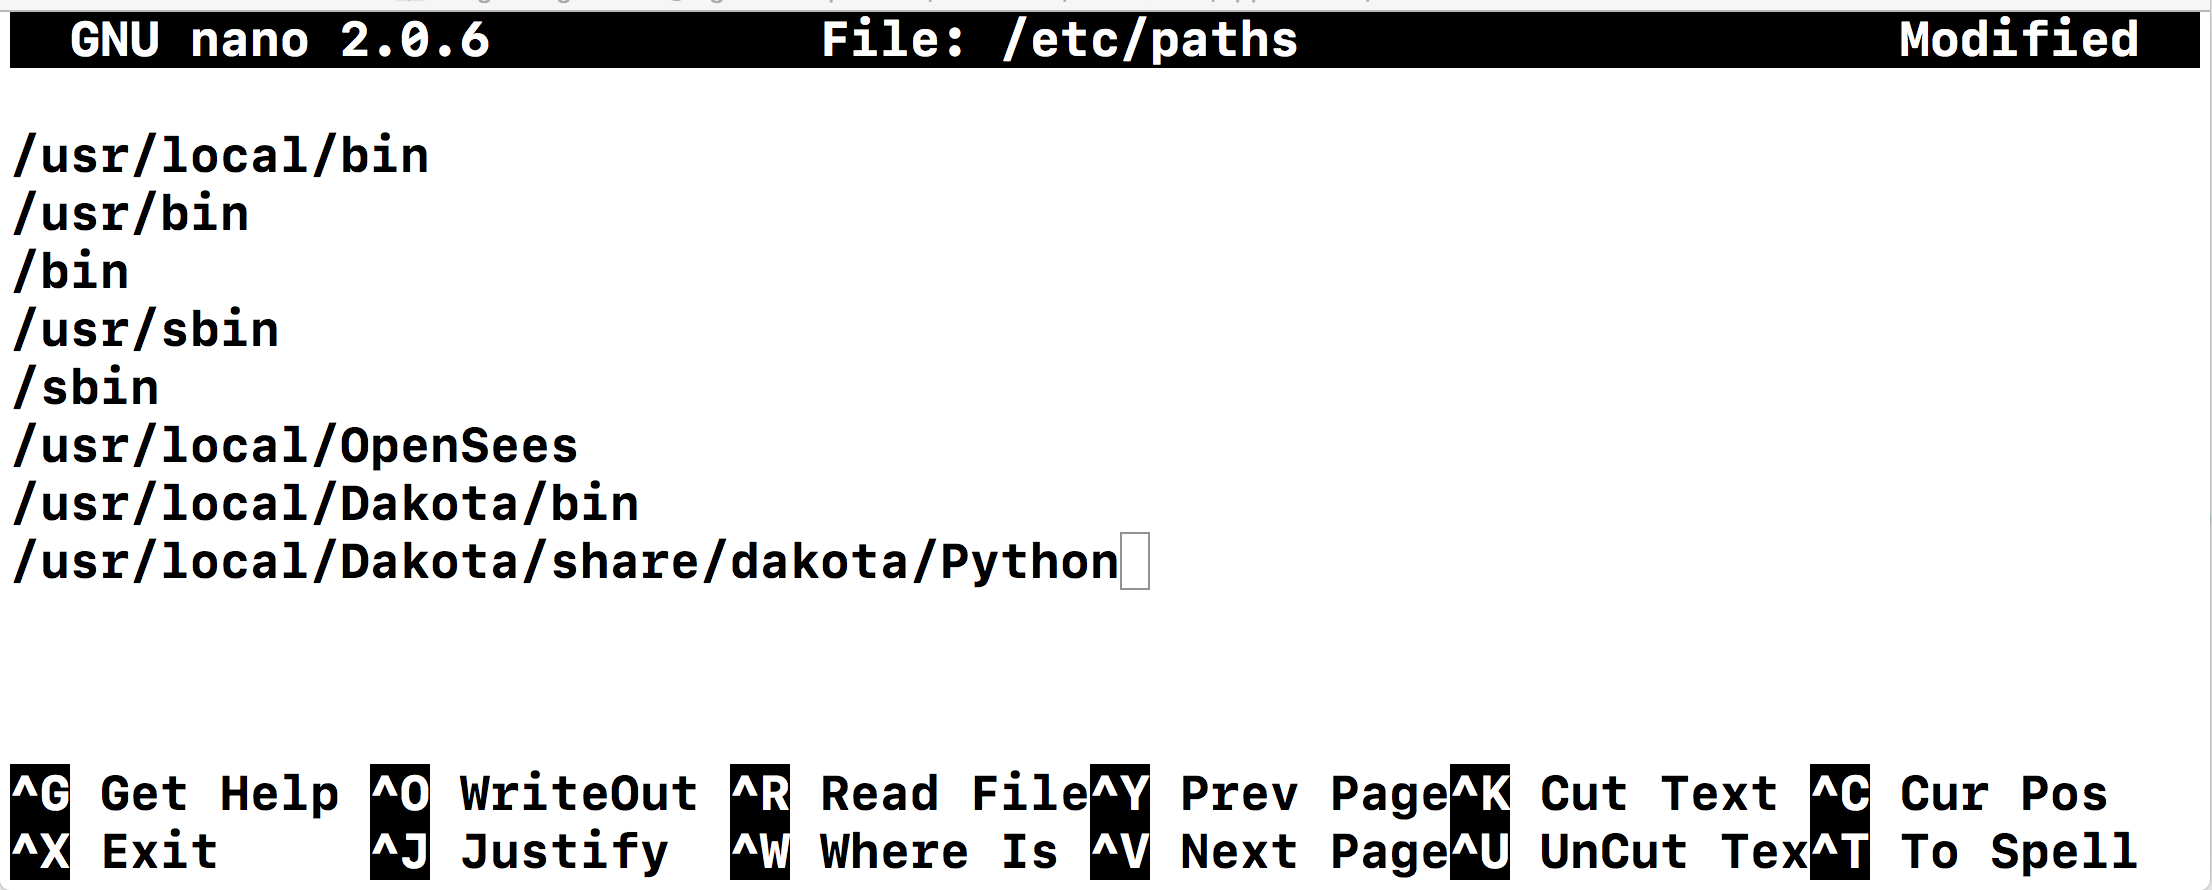
\includegraphics[width=0.8\textwidth]
    {installation/figures/add_env_path_Mac.png} }
  \caption{Adding OpenSees to the PATH environment variable on Mac.}
  \label{fig:add_env_path_Mac}
\end{figure}
\end{enumerate}


\subsection{Install \texttt{Dakota}}
%===============================================================================

\href{http://dakota.sandia.gov}{\texttt{Dakota}}, an open-source  optimization and UQ application from Sandia National Labs, is publicly available for download at its \href{http://dakota.sandia.gov/download.html}{download page}. Select your operating system from the list and set the other options as shown in  \Cref{fig:dakota_installation}. Download the release in a \texttt{ZIP} file for Windows and \texttt{TAR.GZ} file for Mac. We recommend you to extract the archive to a \texttt{C:/SimCenter/Dakota} folder on Windows, and to a \texttt{/usr/local/Dakota} folder on a Mac.

\begin{figure}[!htbp]
  \centering {
    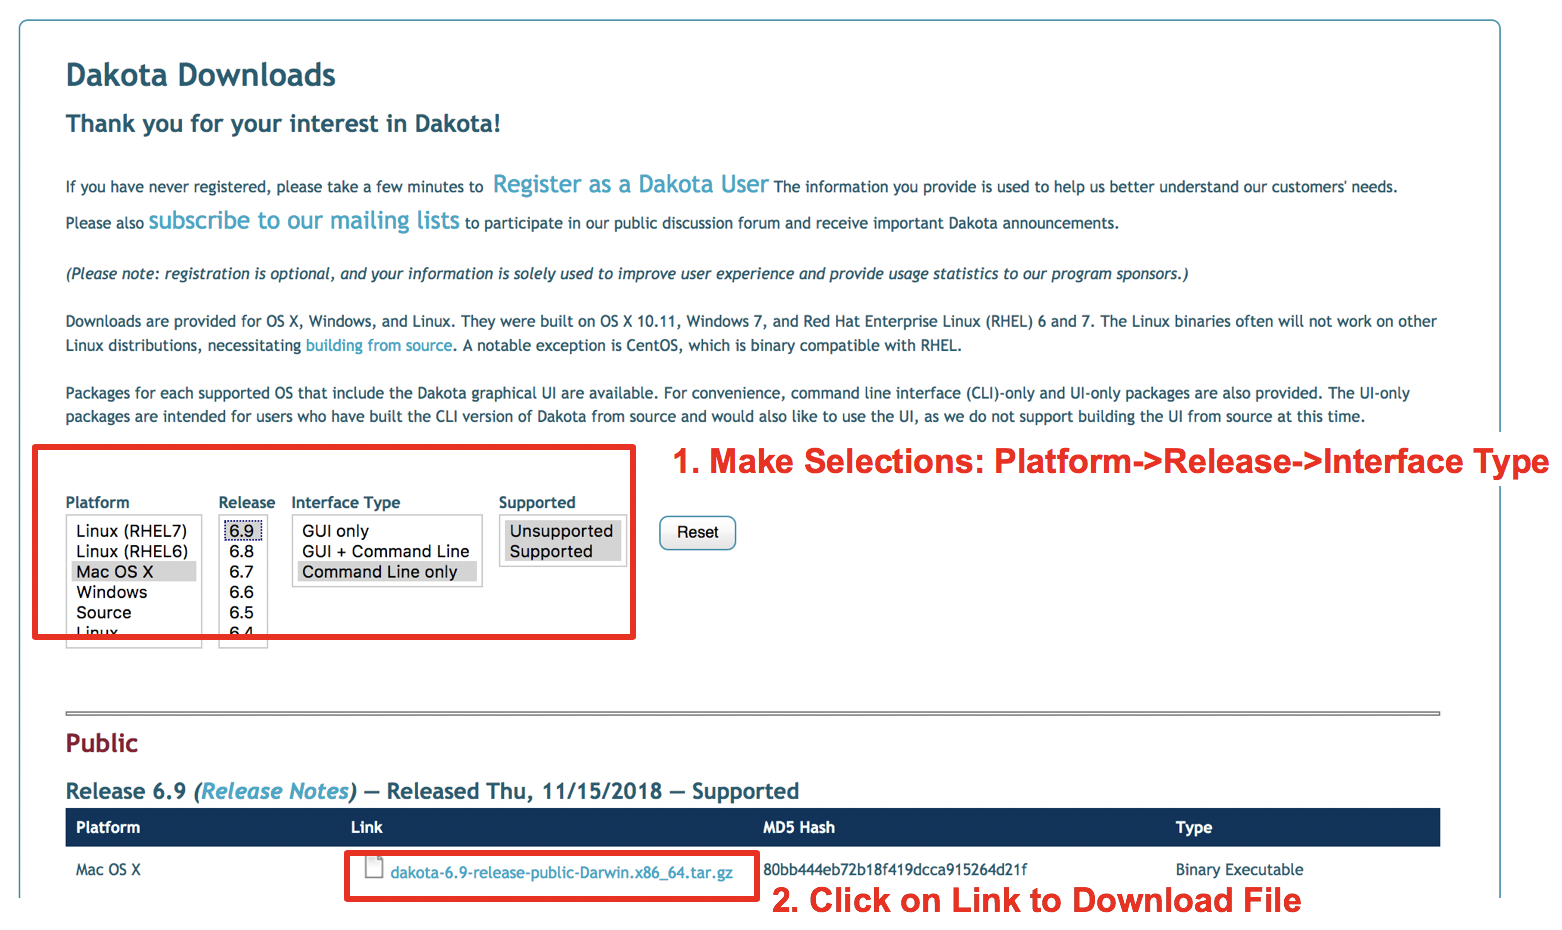
\includegraphics[width=\textwidth]
    {installation/figures/dakota_installation.png} }
  \caption{Downloading Dakota Software}
  \label{fig:dakota_installation}
\end{figure}

Following the instructions provided for installing \texttt{OpenSees}, you need to add \textbf{two} \texttt{Dakota} folders to the system \texttt{PATH} environment variable to allow the SimCenter
workflow applications to find the \texttt{Dakota} tools on your computer. Use
the procedure described above for \texttt{OpenSees} to add the following
folders to your \texttt{PATH}:

\begin{enumerate}
\item Windows:
\begin{itemize}
    \item \texttt{C:\textbackslash SimCenter\textbackslash Dakota\textbackslash bin}
    \item \texttt{C:\textbackslash SimCenter\textbackslash Dakota\textbackslash share\textbackslash dakota\textbackslash Python}
\end{itemize}

\item MacOS:
\begin{itemize}
    \item \texttt{/usr/local/Dakota/bin}
    \item \texttt{/usr/local/Dakota/share/dakota/Python}
\end{itemize}
\end{enumerate}

In addition to modifications to the \texttt{PATH} environment variable, you need to create/modify another variable. This new variable name is \texttt{PYTHONPATH}. To add an environment variable on a Mac you need to edit the \texttt{.bashrc} file in your home directory and add the line shown below.

\begin{enumerate}
\item Windows:
\begin{itemize}
    \item \texttt{C:\textbackslash SimCenter\textbackslash Dakota\textbackslash share\textbackslash dakota\textbackslash Python}
\end{itemize}

\item MacOS:
\begin{itemize}
    \item \texttt{export PYTHONPATH=/usr/local/Dakota/share/dakota/Python}
\end{itemize}
\end{enumerate}

\subsection{Install  Perl}
%===============================================================================

Mac OS X has Perl pre-installed, but Windows users will have to
install it to be able to use \texttt{Dakota}. We recommend you use Strawberry
Perl; you can install it by downloading the executable from
its \href{http://strawberryperl.com}{Strawberry Perl website} and
running it.

\subsection{Test the Install of the Local Applications}
%===============================================================================

Before running the \texttt{\getsoftwarename{}} application, perform the following tests to
make sure that the local SimCenter working environment is set up
appropriately:

\begin{itemize}
    \item Start a Terminal on Mac or a Command Prompt on Windows.
    \item On Mac, execute \texttt{cd /usr/Documents} to change the active directory to \texttt{/usr/Documents}. On Windows, execute \texttt{cd C:/} to change the active directory to \texttt{C:/}.
    \item Test if \texttt{OpenSees} works correctly by executing the \texttt{OpenSees} command. The command should start \texttt{OpenSees} (\Cref{fig:opensees_test}). Close \texttt{OpenSees} with the \texttt{exit} command.
    \item Test if \texttt{Dakota} works correctly by executing the \texttt{dakota} command. The command should start \texttt{Dakota} and you should see a message about a missing argument (\Cref{fig:dakota_test}).
    \item Test if Perl works correctly by executing the \texttt{perl -v} command. The command should start Perl and return its version number (\Cref{fig:perl_test}).
    \item Test if the python package in \texttt{Dakota} works correctly by starting Python with the \texttt{python} command and then executing the \texttt{import dakota} command. This should import the dakota package. If you do not see errors, then the package is successfully imported (\Cref{fig:dakota_py_test}). Exit Python with the \texttt{exit()} command.
    \item If all the above tests ran without errors, your environment is set up appropriately.
\end{itemize}

\begin{figure}[!htbp]
  \centering {
    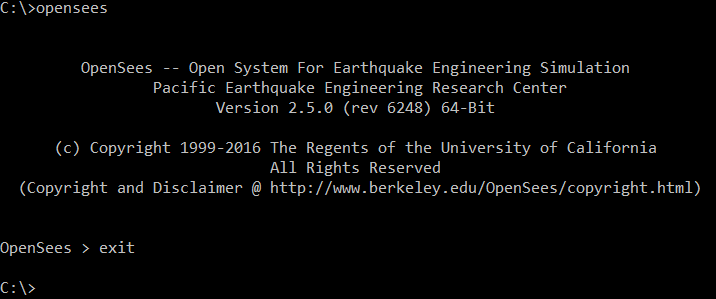
\includegraphics[width=0.8\textwidth]
    {installation/figures/opensees_test.png} }
  \caption{Testing OpenSees.}
  \label{fig:opensees_test}
\end{figure}

\begin{figure}[!htbp]
  \centering {
    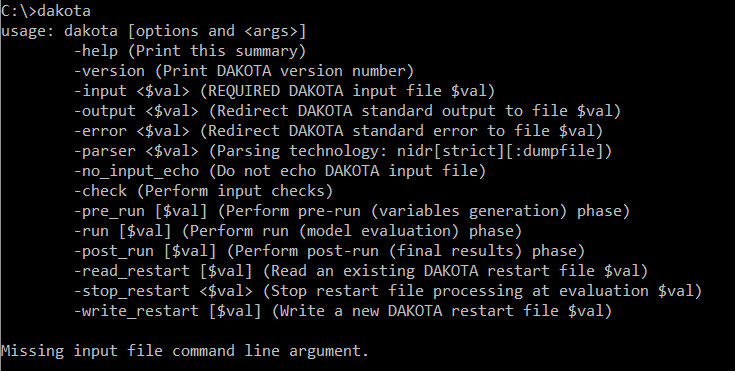
\includegraphics[width=0.8\textwidth]
    {installation/figures/dakota_test.png} }
  \caption{Testing Dakota.}
  \label{fig:dakota_test}
\end{figure}

\begin{figure}[!htbp]
  \centering {
    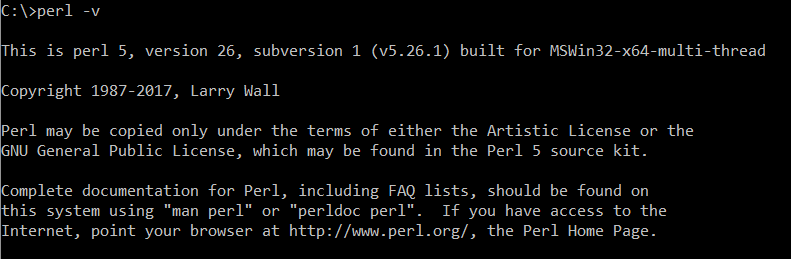
\includegraphics[width=0.8\textwidth]
    {installation/figures/perl_test.png} }
  \caption{Testing Perl.}
  \label{fig:perl_test}
\end{figure}

\begin{figure}[!htbp]
  \centering {
    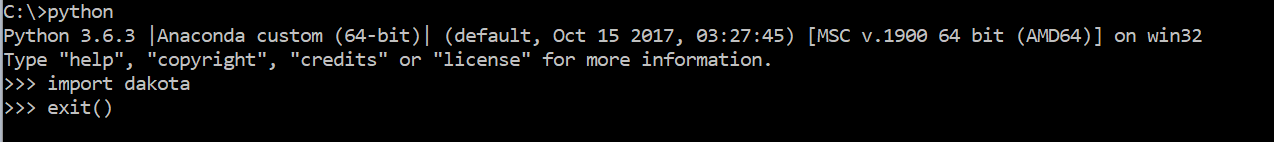
\includegraphics[width=0.8\textwidth]
    {installation/figures/dakota_py_test.png} }
  \caption{Testing the dakota Python package.}
  \label{fig:dakota_py_test}
\end{figure}

%===============================================================================
\clearpage
\section{Test the \texttt{\getsoftwarename{}} application}
\label{sec:test_local}
Once the local SimCenter working environment has been tested and is
functioning correctly, the \texttt{\getsoftwarename{}} Application
can be tested. The simplest way to do this is by running an analysis
using the default structural model with synthetic ground motions. By
doing this, it is not necessary to enter any information on the
structural model and only inputs for 
\softwareSwitch{PBE}{
the synthetic motions, uncertainty quantification, and loss assessment
}{
the synthetic motions and uncertainty quantification
}
are required. With this quick setup, the
functionality of the \texttt{\getsoftwarename{}} App and the backend
workflow can be tested. The necessary steps to perform this
testing are provided below.

A full description of how to use this software is provided
in \Cref{chap:usage}.  In this quick test, users will only
interface with the event tab (\texttt{EVT}), the uncertainty
quantification tab (\texttt{UQ}), 
\softwareSwitch{PBE}{
the damage and loss assessment tab (\texttt{CMP}),
}{}
and the results tab (\texttt{RES}).

The first step is to start the \texttt{\getsoftwarename{}}
application.  Once the application started, the second step is to
input the parameters for the synthetic motions under the \texttt{EVT}
(Event) tab. This is shown in \Cref{fig:input_event}. Click
on the \texttt{EVT} tab which will allow the loading type to be
selected. From the dropdown menu, as shown
in \Cref{fig:input_event}, select \texttt{Stochastic Ground Motion
Model}. Upon selecting this loading type, the loading model will be
set as \texttt{Vlachos et al. (2018)}.

\softwareSwitch{PBE}{
\begin{figure}[!htbp]
  \centering {
    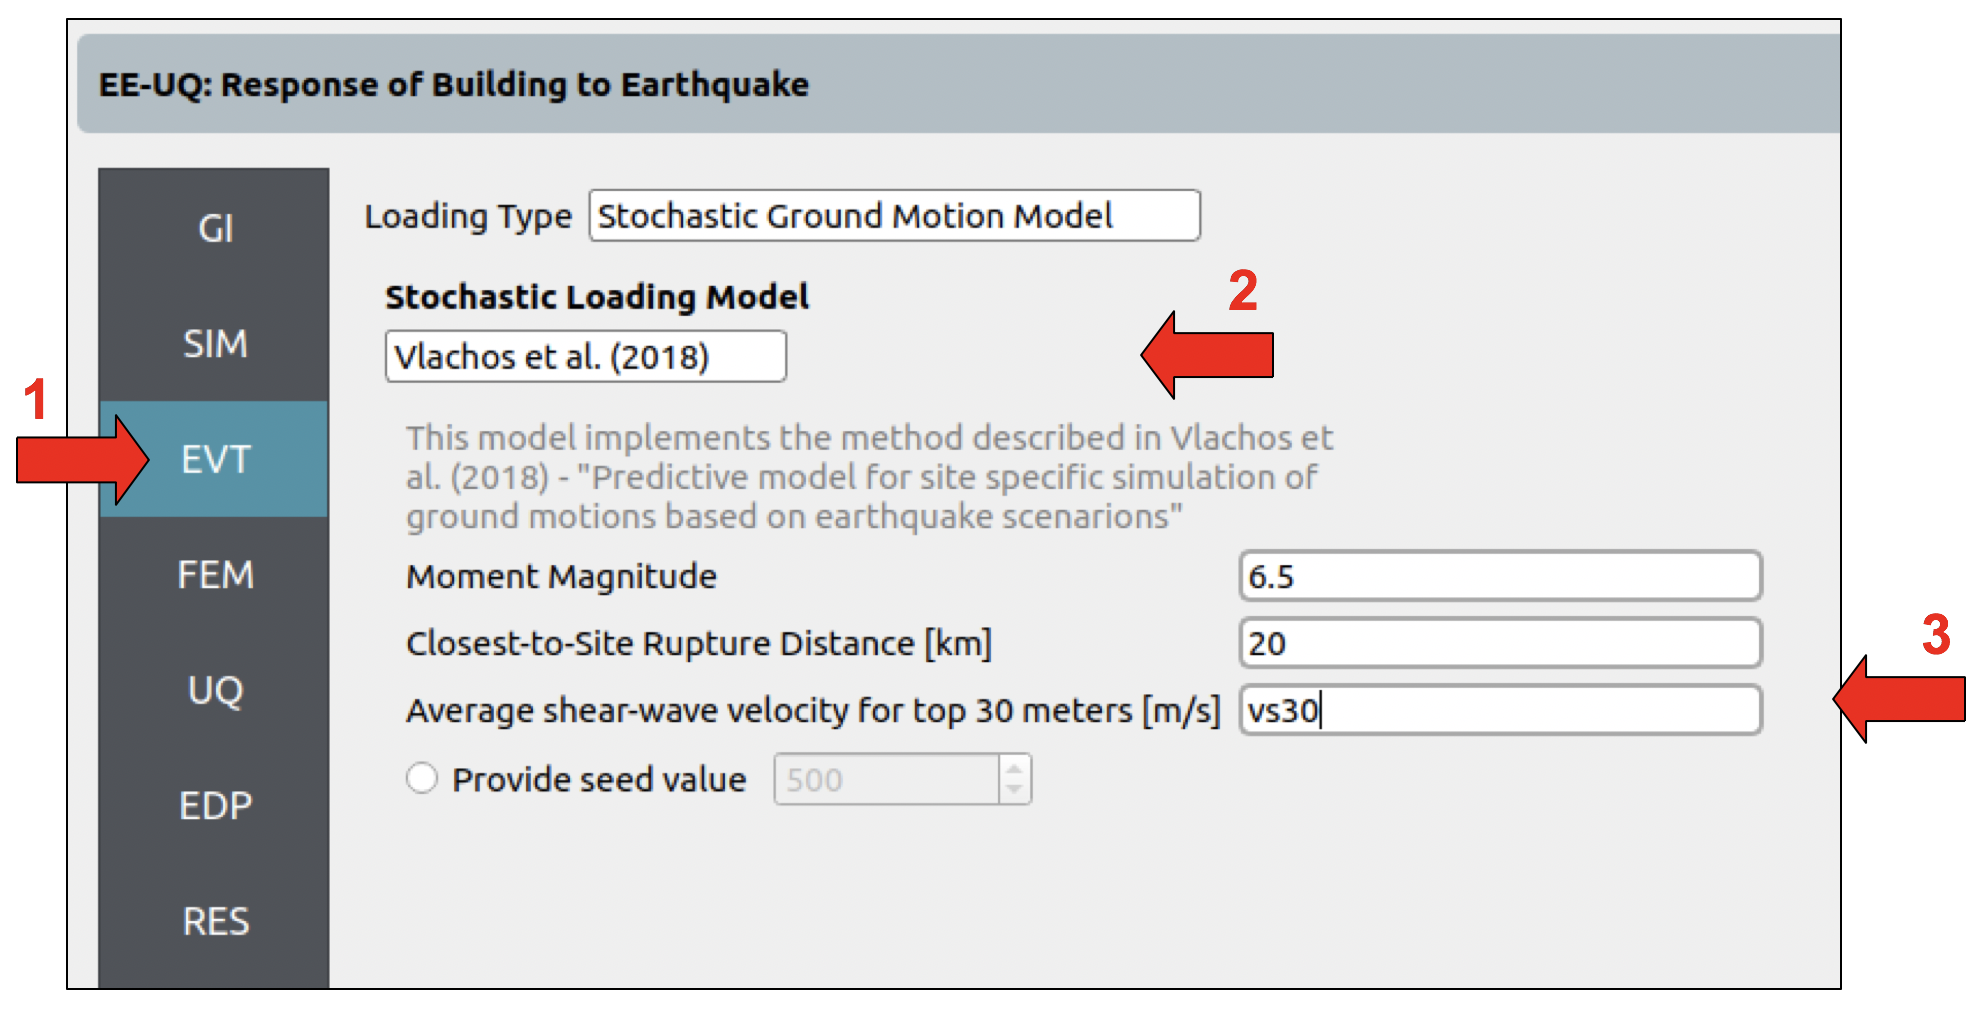
\includegraphics[width=0.7\textwidth]
    {installation/figures/test_input_event.png} }
  \caption{Selecting event type and inputting synthetic motion parameters}
  \label{fig:input_event}
\end{figure}
}{
\begin{figure}[!htbp]
  \centering {
    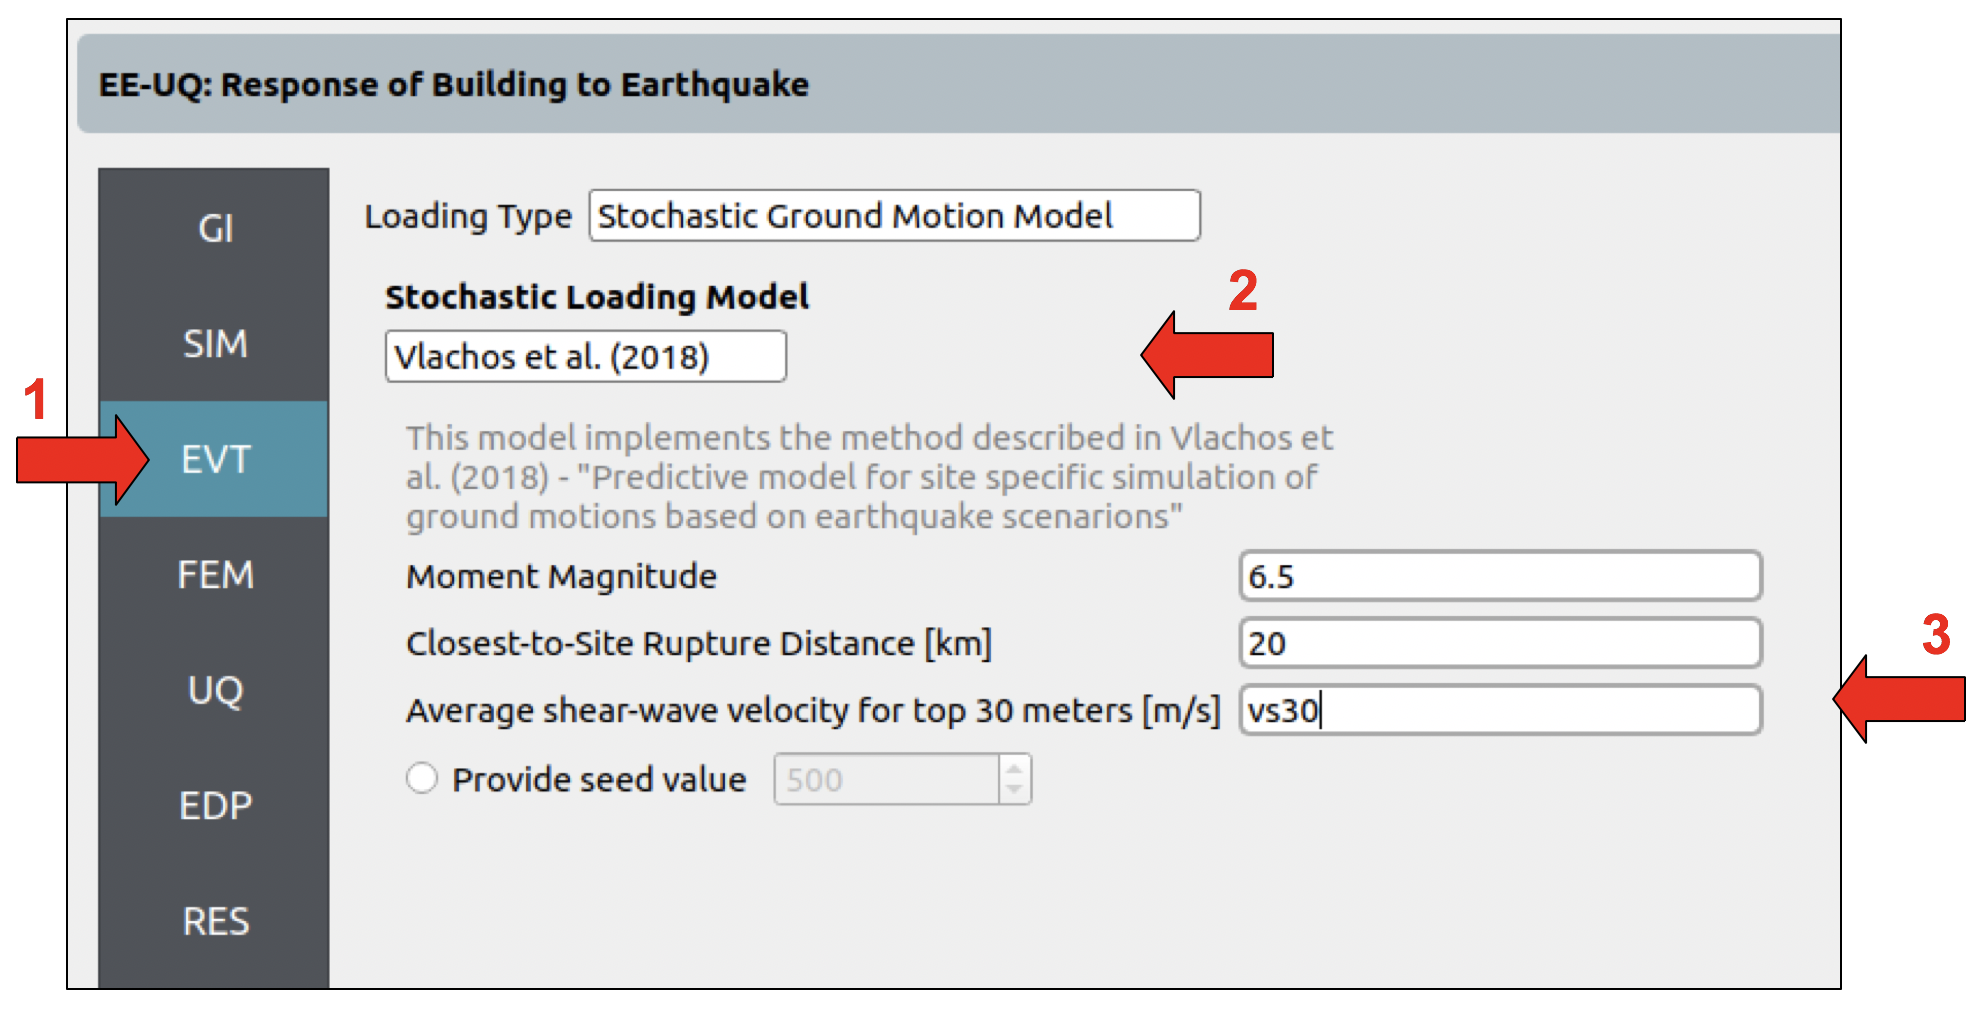
\includegraphics[width=0.7\textwidth]
    {installation/figures/test_input_event.png} }
  \caption{Selecting event type and inputting synthetic motion parameters}
  \label{fig:input_event}
\end{figure}
}

Only three inputs are required for this test, of which one will be set
to a random variable. As shown in \Cref{fig:input_event}, set the
\emph{Moment Magnitude} ($M_W$) to 6.5, the \emph{Closest-to-Site Rupture Distance}
($R_{rupt}$) to 20 km, and the \emph{Average shear-wave velocity
for the top 30 m} ($V_{S_{30}}$)
to \texttt{vs30}. The \texttt{Provide seed value} radio button should
be left unselected. By specifying these inputs, both $M_{W}$ and $R_{rupt}$
will have constant values in all realizations while $V_{S_{30}}$ will
have different values based on the model parameters specified in the
uncertainty quantification (\texttt{UQ}) tab.

With these inputs specified, navigate to the \texttt{UQ} tab. Here the
distributions and their relevant parameters will be specified for the
random variables defined in the analysis\textemdash only $V_{S_{30}}$
in this case. Since $V_{S_{30}}$ was identified as a random variable
by inputting the parameter value as text, it is automatically added as
a random variable, as shown in \Cref{fig:input_uq}. Set the
distribution type to \texttt{normal} with a \texttt{Mean}
and \texttt{Standard Dev} of 350 m/s and 25 m/s,
respectively.

\softwareSwitch{PBE}{
\begin{figure}[!htbp]
  \centering {
    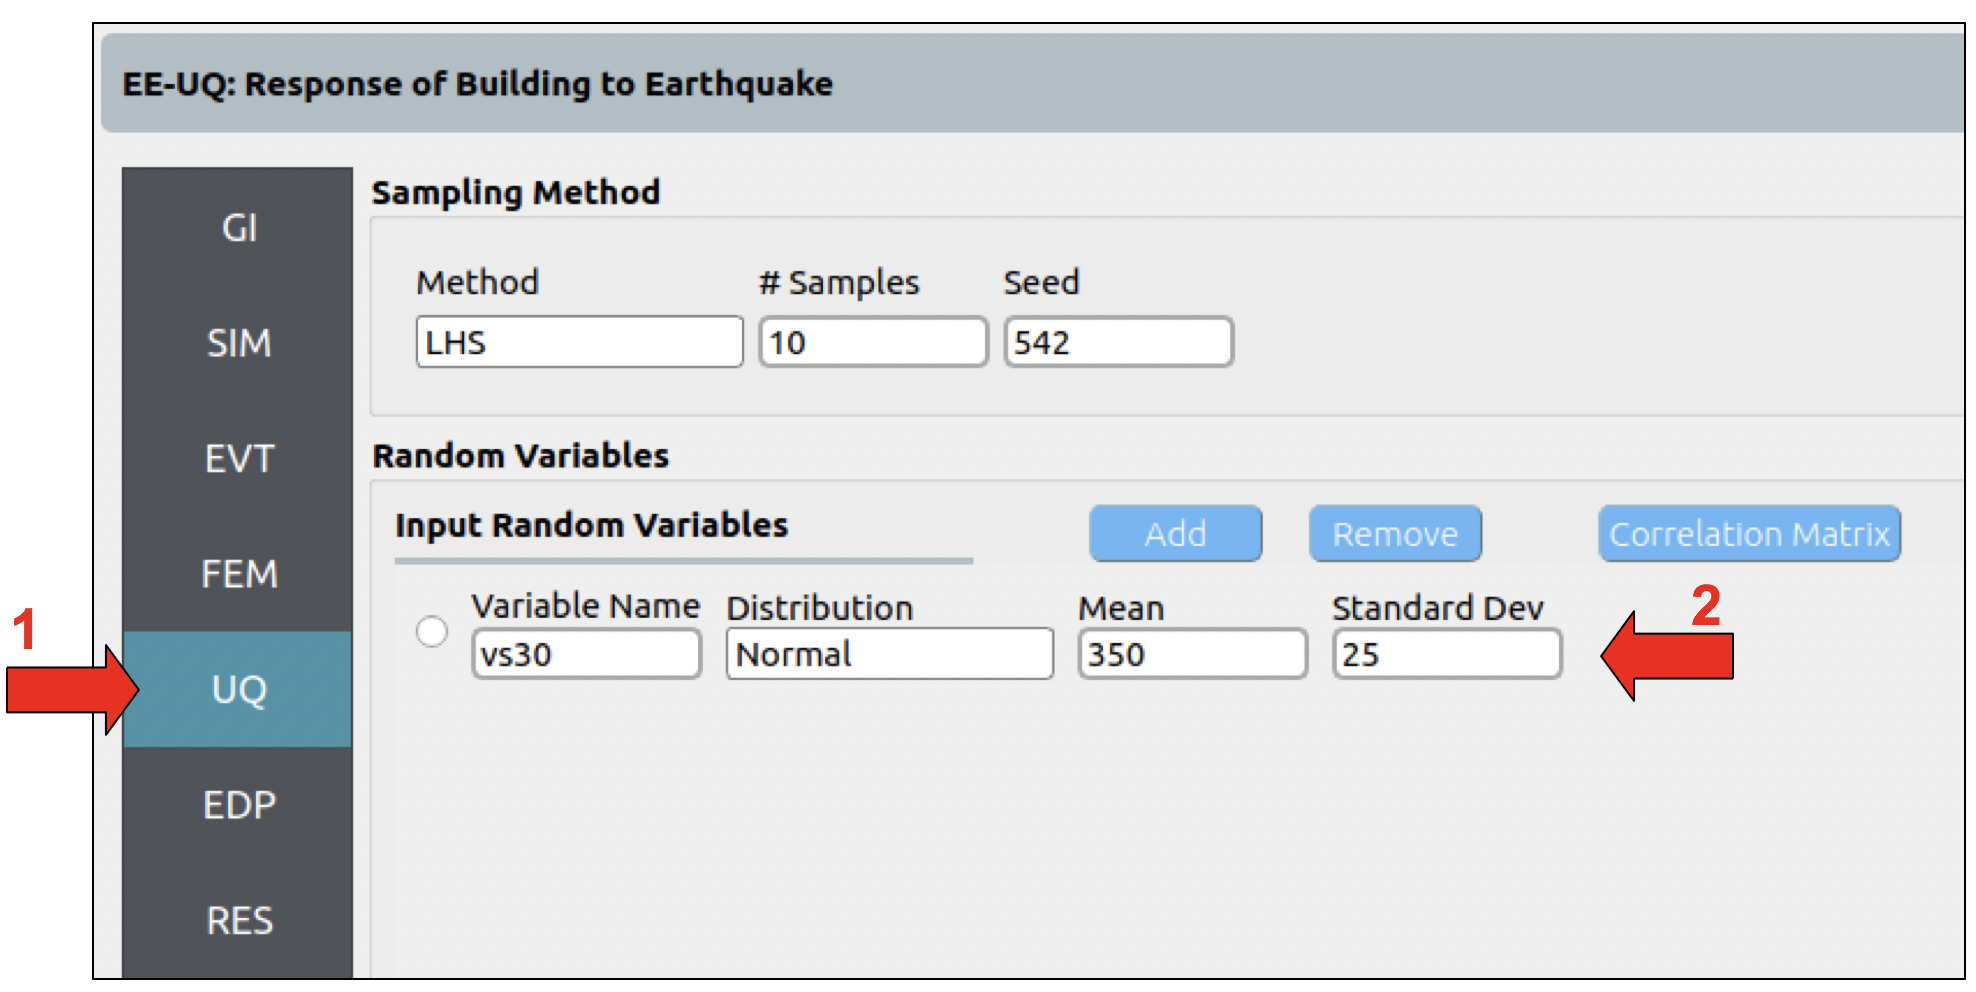
\includegraphics[width=0.7\textwidth]
    {installation/figures/test_input_uq.png} }
  \caption{Specifying distribution type and parameters for random
  variables in analysis\textemdash only $V_{s30}$ in this case}
  \label{fig:input_uq}
\end{figure}
}{
\begin{figure}[!htbp]
  \centering {
    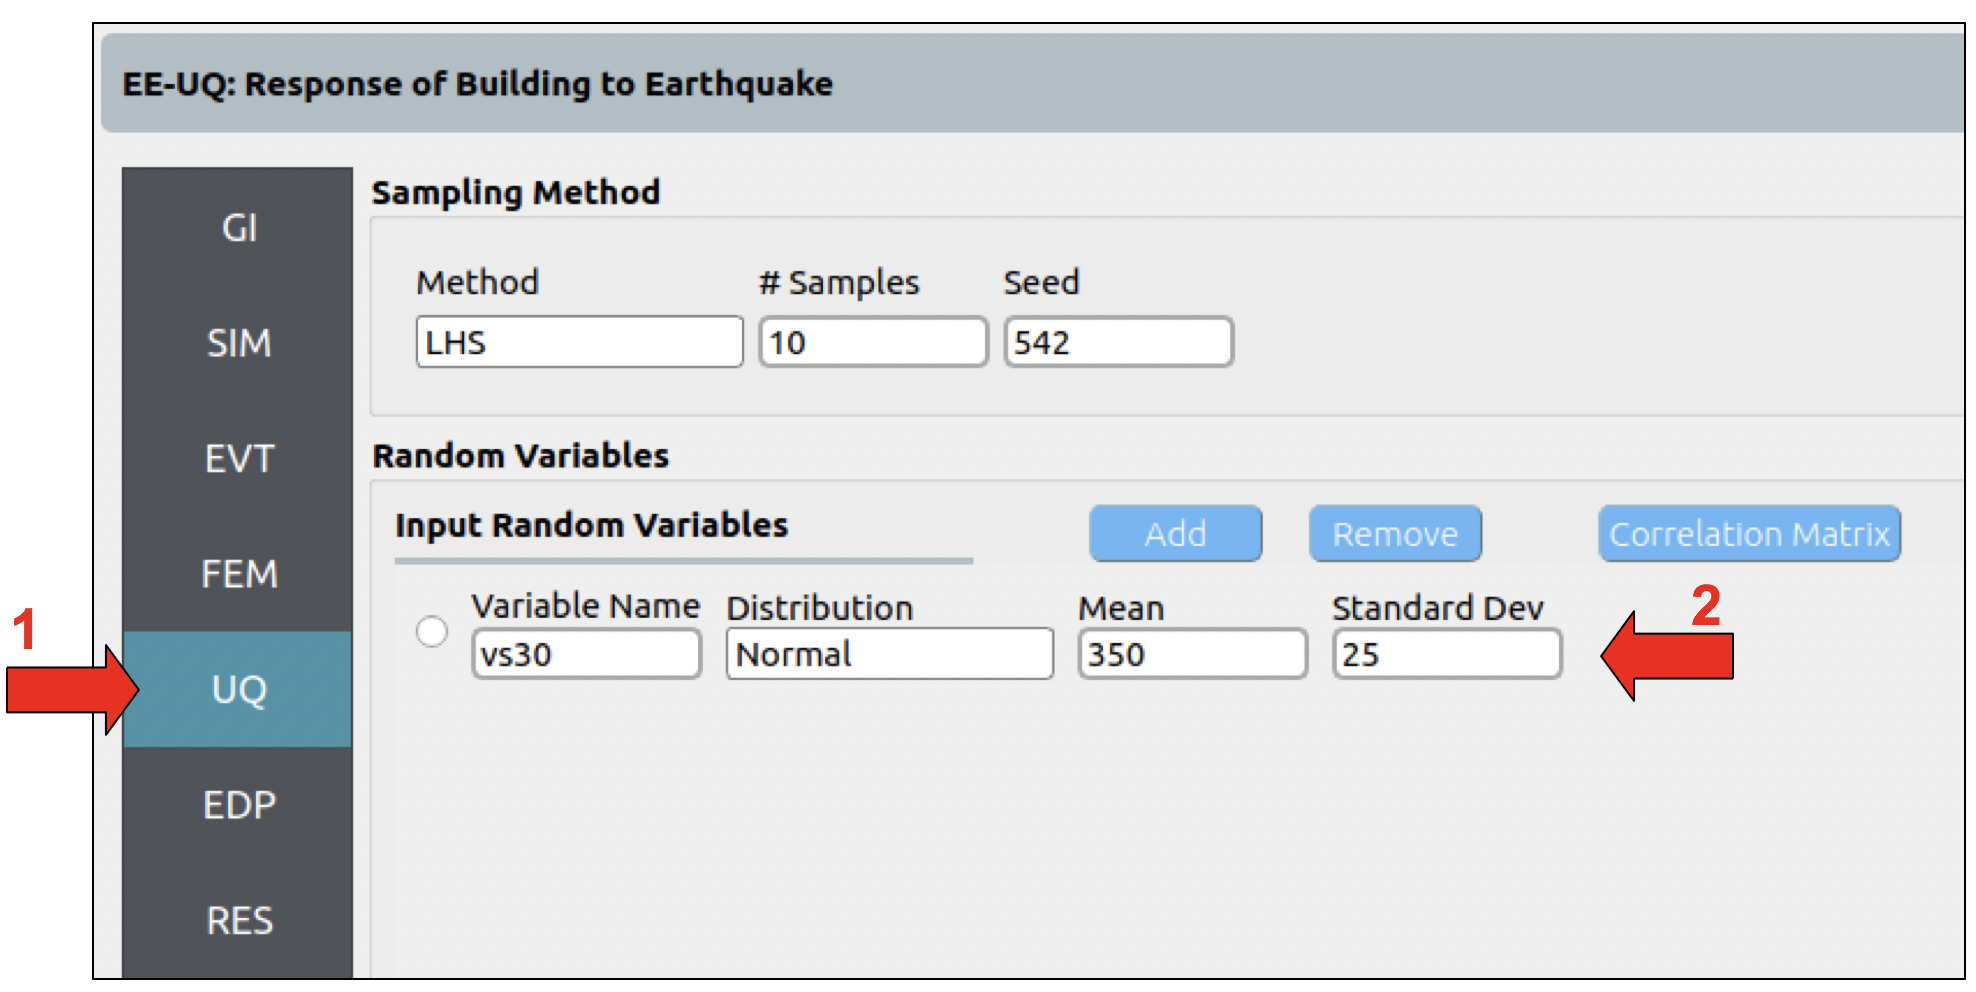
\includegraphics[width=0.7\textwidth]
    {installation/figures/test_input_uq.png} }
  \caption{Specifying distribution type and parameters for random
  variables in analysis\textemdash only $V_{s30}$ in this case}
  \label{fig:input_uq}
\end{figure}
}

\softwareSwitch{PBE}{
The last step before running the analysis is to set up a damage and loss model. Navigate to the \textttt{CMP} tab and select \texttt{HAZUS MH} as the loss assessment method to use. Set up the model according to \Cref{fig:input_dl}.
\begin{figure}[!htbp]
  \centering {
    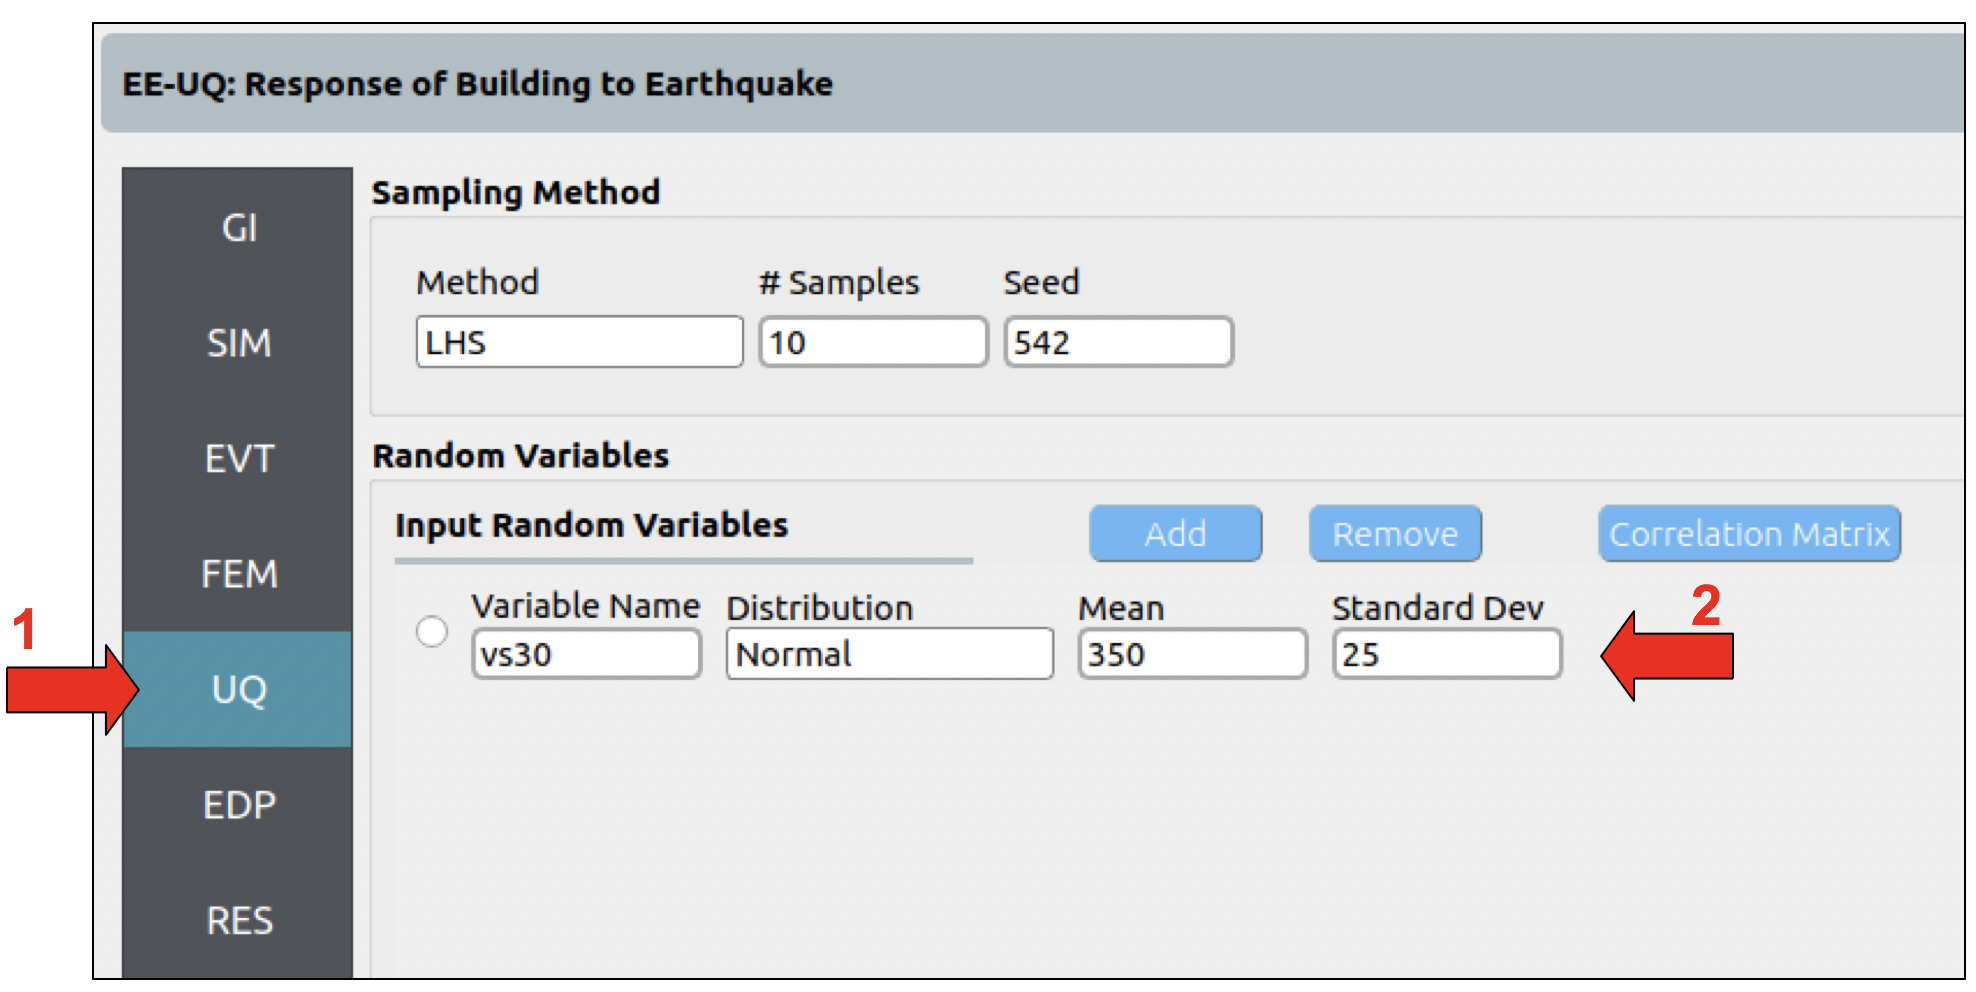
\includegraphics[width=0.7\textwidth]
    {installation/figures/test_input_uq.png} }
  \caption{Specifying the damage and loss model for the analysis.}
  \label{fig:input_dl}
\end{figure}
}{}

Now, click on the \texttt{RUN} button, which will bring up a pop-up
menu that provides information on the application directory and
the working directory. The application directory should already be
automatically set to where \texttt{\getsoftwarename{}} is installed.
If desired, the working directory can be changed. In order to start
the analysis, click on the \texttt{Submit} button.

\softwareSwitch{PBE}{
\begin{figure}[!htbp]
  \centering {
    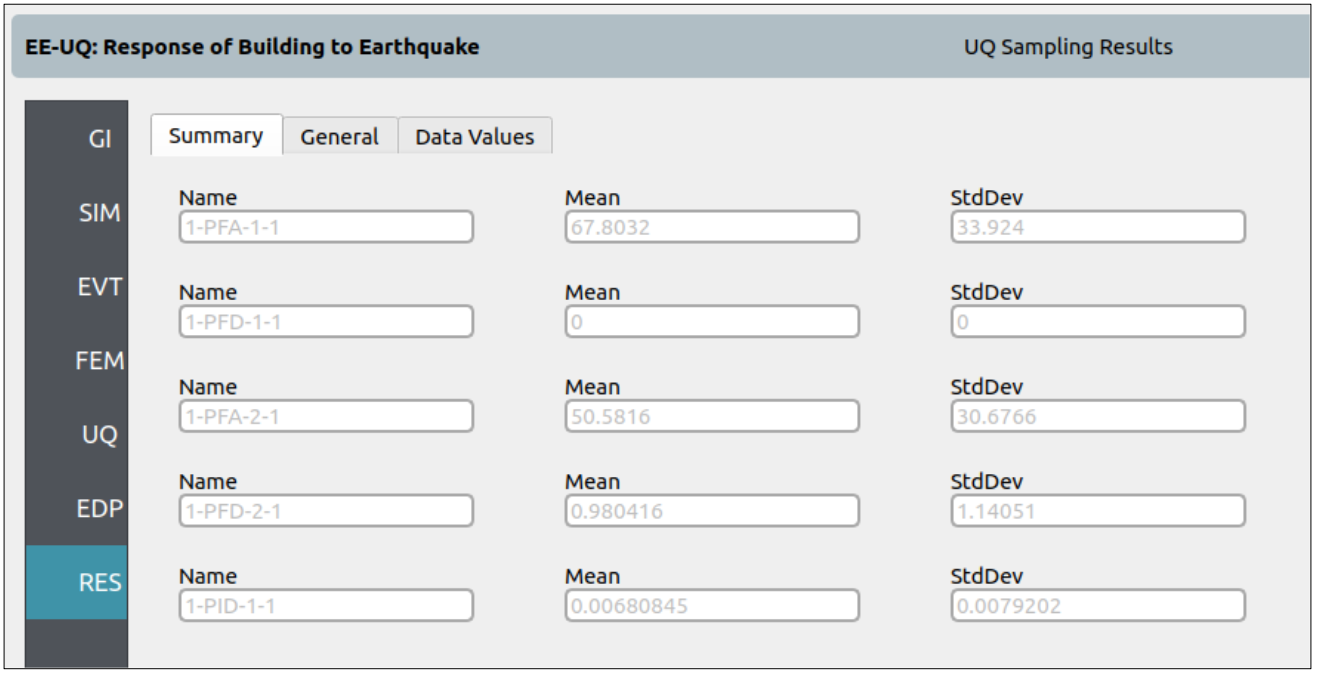
\includegraphics[width=0.7\textwidth]
    {installation/figures/test_uq_res.png} }
  \caption{Results for test analysis. This tab will open automatically
  when the analysis completes, indicating a successful installation}
  \label{fig:show_results}
\end{figure}
}{
\begin{figure}[!htbp]
  \centering {
    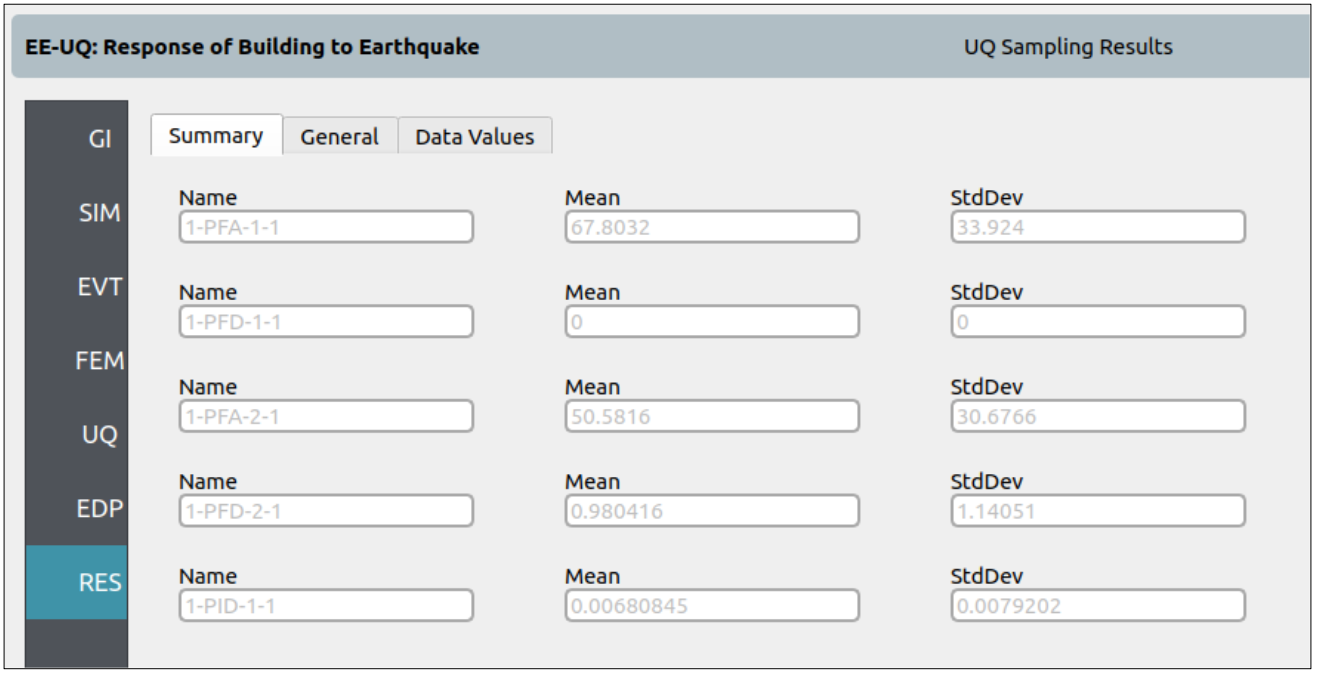
\includegraphics[width=0.7\textwidth]
    {installation/figures/test_uq_res.png} }
  \caption{Results for test analysis. This tab will open automatically
  when the analysis completes, indicating a successful installation}
  \label{fig:show_results}
\end{figure}
}

If successful, the application will pause briefly while it runs the
analysis before automatically displaying the simulations results in
the \texttt{RES} tab, as shown
in \Cref{fig:show_results}. Remember, the results shown
in \Cref{fig:show_results} most likely will not be the same as
those from this local test since $V_{S_{30}}$ is a random variable and
the values realized in the simulations will be different while still
following the same distribution. In any case, if the simulations
completed and the \texttt{RES} tab is showing simulation results, then
the \texttt{\getsoftwarename{}} App is properly installed and configured.

%===============================================================================



%\chapter{Usage}
%\label{chap:usage}
%\section{User Interface}
The user interface (UI), as shown in \Cref{fig:figure1}, is where the analysis
is configured and managed. Here, the user is able to provide the necessary
parameters to create the simulation, start the simulation both locally and
remotely, and view the simulation results. The interface contains several
separate areas:

\begin{figure}[!htbp]
  \centering {
    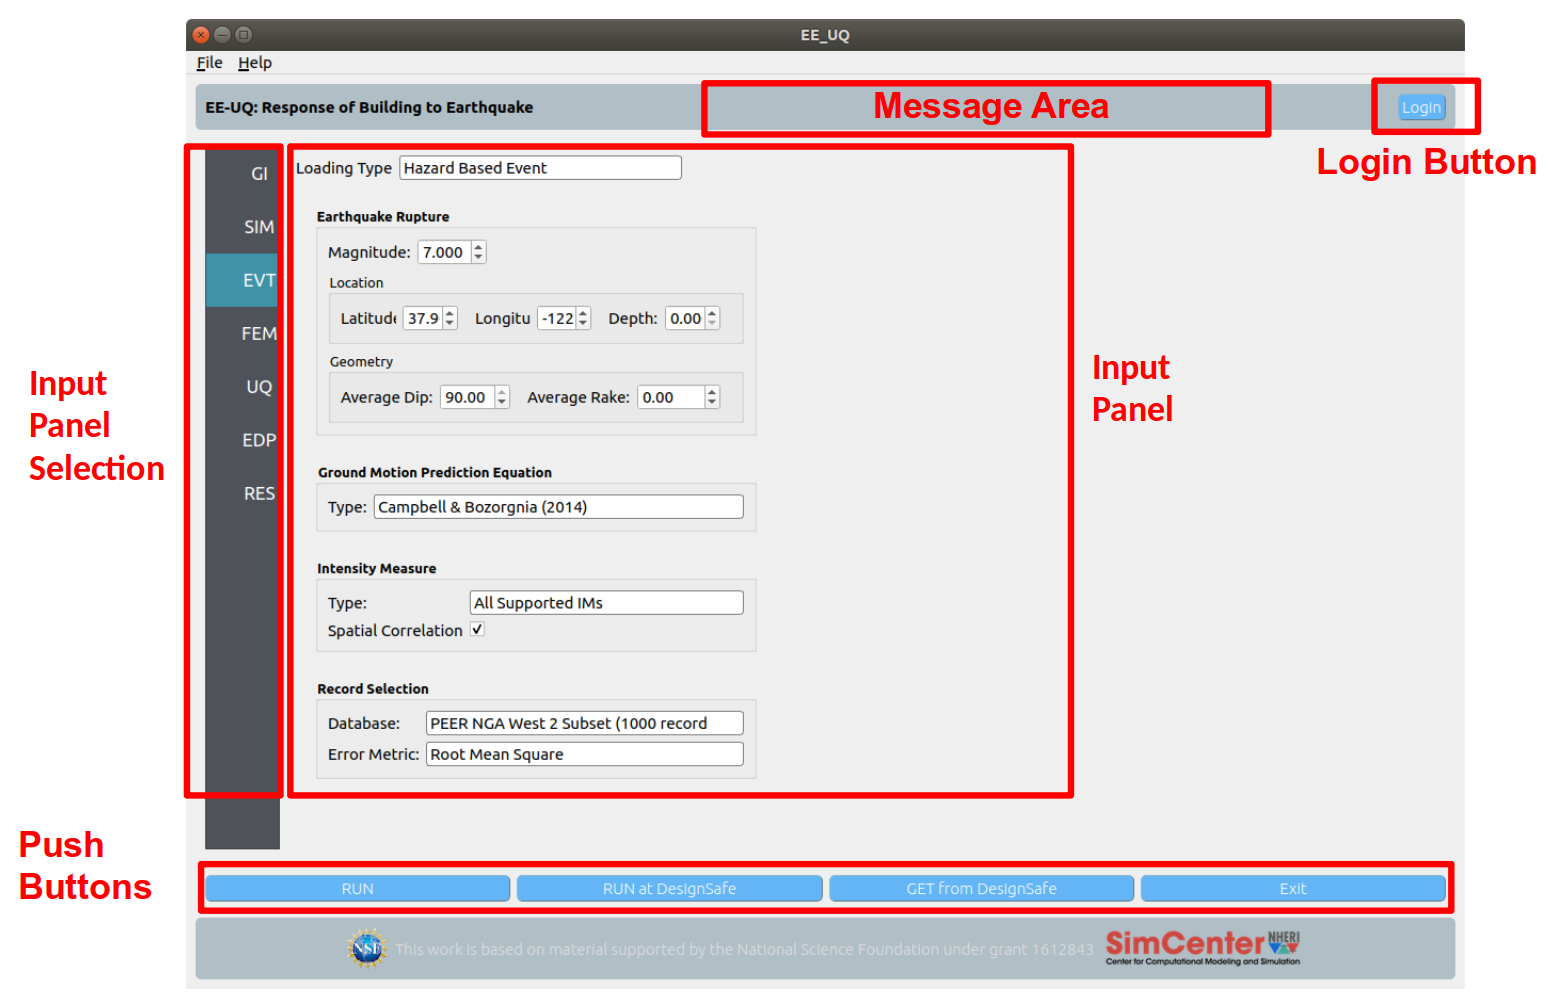
\includegraphics[width=0.8\textwidth]
    {usage/figures/ui.png} }
  \caption{UI}
  \label{fig:figure1}
\end{figure}

\begin{enumerate}
\item Input Panel Selection: This area on the left side provides the
  user with a selection of items to choose from from:
\begin{enumerate}
  \item GI: General Information (\ref{sec:generalInfo}), for specifiction of building
    description, location and units.
  \item SIM: Structure Information Model (\ref{sec:structuralInfo}), for description of the
    building model.
  \item EVT: Event (\ref{sec:event}), for selecting the input earthquake motions for building.
  \item FEM: Finite element method (\ref{sec:fem}), for specifying the analysis options.
  \item UQ: Uncertainty quantification (\ref{sec:uq}), for defining the distribution
    of the random variable paramaters and UQ method analysis options.
  \item EDP: Engineering Demand Parameters (\ref{sec:edp}), for specification of
    output response quantities.
  \item RES: Results output (\ref{sec:results}), for looking at the results.
\end{enumerate}

Selecting any of these will change the input panel presented.

\item Input Panel: This is the large central area of the UI that the
  user provides input for the application chosen and views the
  results. For example if the user had selected UQ in the input panel
  selection, it is in this panel that the user would provide details
  on the distributions associated with each random variable or select
  the sampling method to use and provide the options necessary to run
  that method.

\item Push Buttons: This is the area near the bottom of the UI in
  which 4 buttons are presented to the user:

\begin{enumerate}
\item RUN – to run the simulation of the user’s desktop machine.
\item RUN at DesignSafe – to process the information, and send to
  DesignSafe where the job will be run on a supercomputer and results
  stored in your DesignSafe jobs folder.
\item GET from DesignSafe – to obtain from DesignSafe your list of
  jobs and select from that list a job to download.
\item Exit: to exit the application.
\end{enumerate}

The use of the push buttons is discussed in \Cref{sec:push_buttons}.

\item Login Button: At the top right of the UI is the login
  button. Before the user can launch any jobs on DesignSafe, they must
  first login to DesignSafe using their DesignSafe login and
  password. Pressing the login button will open up the login window
  for users to enter this information. Users can register for an
  account on
  the \href{https://www.designsafe-ci.org/account/register/}{DesignSafe
  webpage}.

\item Message Area: In the top center of the application is the area
  of the interface that error and status messaged will be displayed
  while the application is running.

\end{enumerate}


\section{GI: General Information}
The user here provides information about the building and the units
the user will work in. The widget itself presents 3 separate frames,
as shown in \autoref{fig:figure2}, to the user:

\begin{enumerate}
\item Building Information frame in which user provide general information about the building, this include year of construction and type.
\item Properties frame in which user provides information about number of stories, width, depth, plan area and height of the building.
\item Location frame in which user provides location of the building. This information is used in some of event widgets to obtain events specific to the building.
\item Units frame  in which user specifies what the units will be for the inputs and outputs. Some widgets will require inputs in different units. These entries will contain units beside the specific entry to mark this.
\end{enumerate}


\begin{figure}[!htbp]
  \centering {
    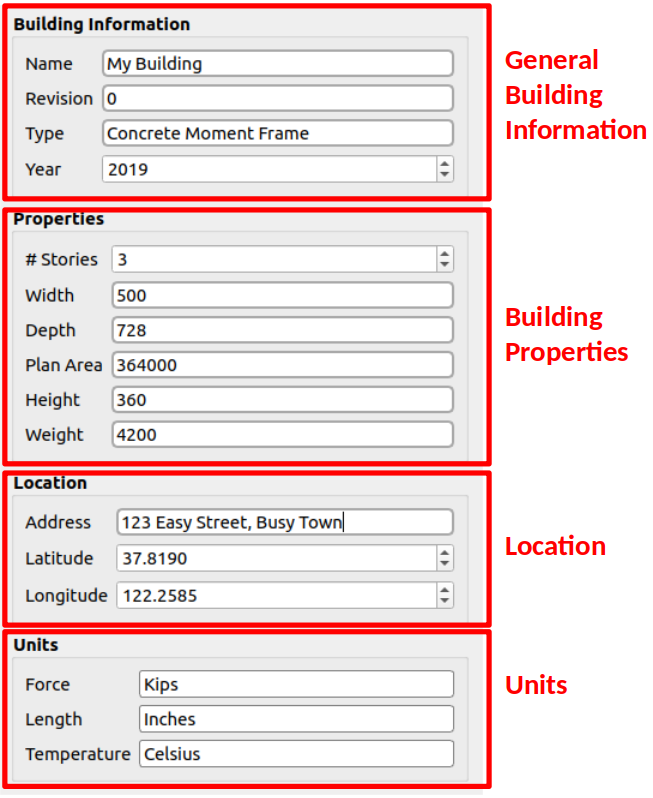
\includegraphics[width=0.5\textwidth]
    {usage/figures/gi.png} }
  \caption{BIM}
  \label{fig:figure2}
\end{figure}



\section{SIM: Structural Information Model}
This panel is where the user defines the structural model of the
building. The structural model is that part of the building provided
to resist the lateral loads. There are a number of backend
applications provided for this part of the workflow, each responsible
for providing the structural analysis model to the workflow. The
drop-down menu at the top of this panel is where the user selects
which application to use. As the user switches between applications,
the entry data changes to reflect the different inputs the different
applications require. At present there are two backend applications
available through the drop down menu: 

\begin{enumerate}
\item Multiple Degrees of Freedom (MDOF) (\ref{sec:MDOF})
\item \texttt{OpenSees} (\ref{sec:OpenSeesSIM})
\end{enumerate}

\subsection{Multiple Degrees of Freedom (MDOF)}\label{sec:MDOF}

This panel is provided for users to quickly create simple shear models
of a building. The panel, as shown in \Cref{fig:mdof} is divided
into 3 frames:
\begin{enumerate}
\item In the top left frame the user enters the number of stories. For
  each story the user then enter the story height, initial stiffness in
  1 and 2 directions, yield strength in the 1 and 2 directions, and
  hardening ratio again in the 1 and 2 directions. Here, the 1 and 2 directions
  are the orthogonal $x$ and $y$ axes in plan view. In addition, user enters
  the floor weights and damping ratios for each of the nodes.
\item In the lower left frame the user has the option of overriding an
  individual floor or story basis, or any of the properties set in the
  upper frame.
\item On the right side of the frame is a graphical widget showing the
  current building. When entering data into the lower left frame,
  those floors and stories corresponding to data being modified is
  highlighted in red.
\end{enumerate}

\begin{figure}[!htbp]
  \centering {
    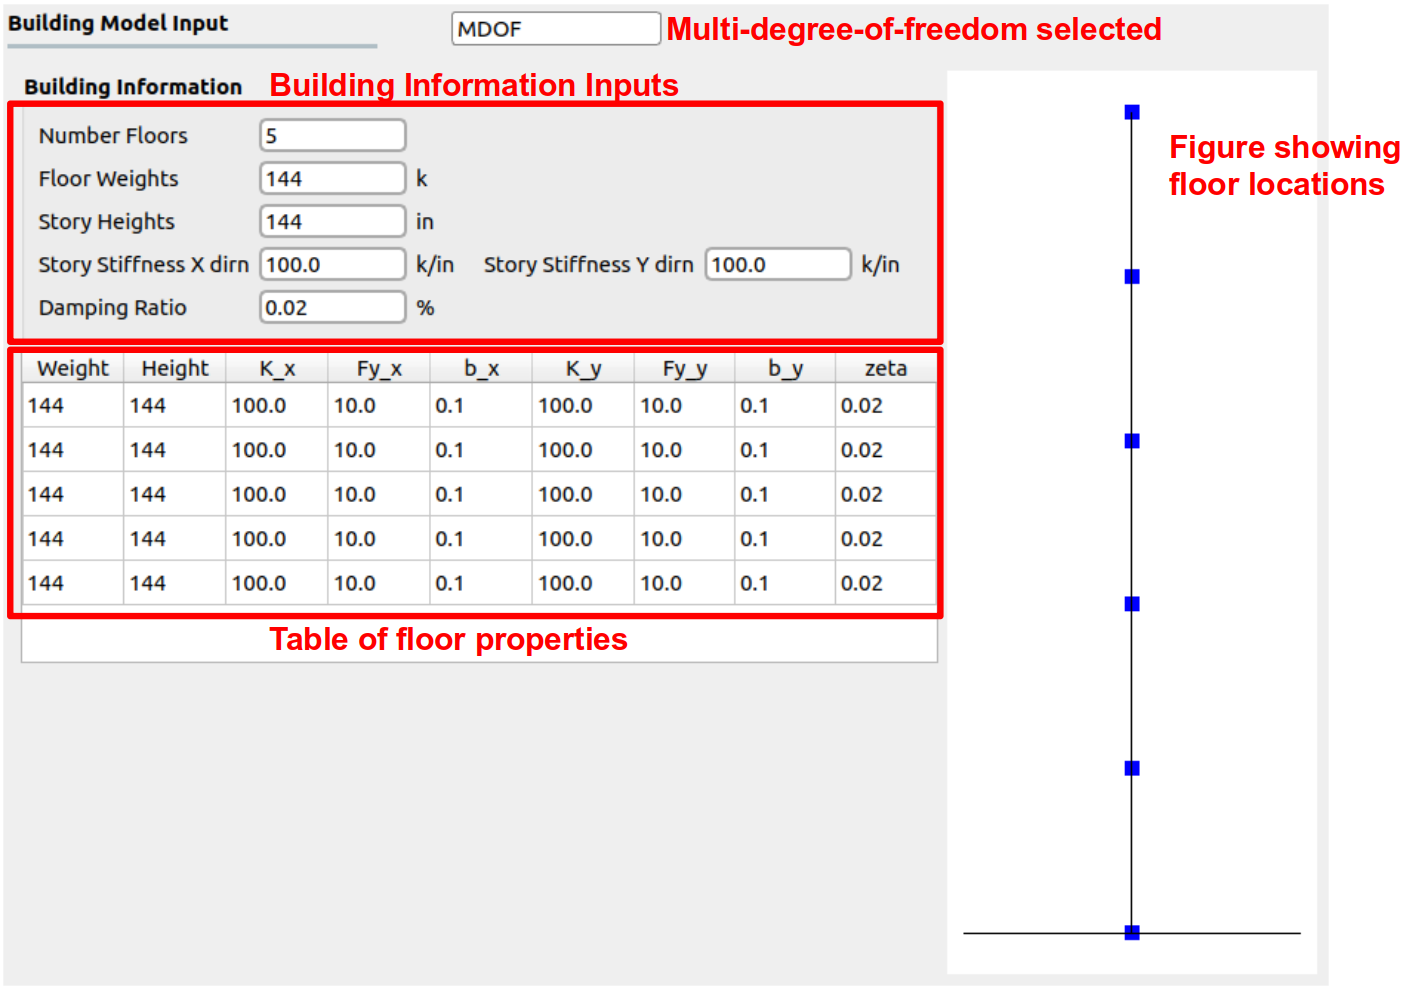
\includegraphics[width=0.8\textwidth]
    {usage/figures/mdof.png} }
  \caption{MDOF or Shear Building Model}
  \label{fig:mdof}
\end{figure}

Random Variables: Random Variables can be created by the user entering
a valid string instead of a number in the entry fields for all entries
except the number of floors. The variable name entered will appear as
a Random Variable in the UQ panel and it is there that the user must
enter the distribution for the Random Variable.

\subsection{\texttt{OpenSees}}\label{sec:OpenSeesSIM}
This panel is for users who have an existing \texttt{OpenSees} model of a
building that performs a gravity analysis and now wish to subject that
building model to one of the \texttt{EVT} options provided. The input panel
for this option is shown in \Cref{fig:figure3}. The user has 3 fields
that they need to complete:
\begin{enumerate} 
\item The user specifies the main script that contains the building
  model. This script should build a model and perform any gravity
  analysis of the building that is required before the event is
  applied.
\item A list of nodes that define a column line of interest for which
  the responses will be determined. The column nodes should be in
  order from ground floor through to roof. The EDP options, described
  in \Cref{sec:edp}, use this information to determine nodes at which
  displacement, acceleration and story drifts are calculated.
\item An entry for the dimension of the model, i.e. 1D, 2D or 3D. This
  information is used to apply ground motions.
\end{enumerate}

\begin{figure}[!htbp]
  \centering {
    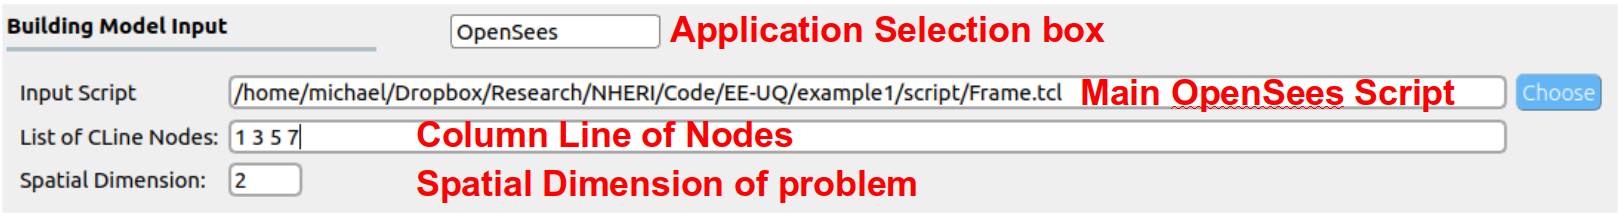
\includegraphics[width=0.8\textwidth]
    {usage/figures/openSees.png} }
  \caption{\texttt{OpenSees} Model}
  \label{fig:figure3}
\end{figure}

Random Variables: In \texttt{OpenSees} there is an option to set
variables to have certain values using the \texttt{pset} command, e.g
\texttt{pset a 5.0} will set the variable a to have a value 5 in an
\texttt{OpenSees} script. In \texttt{\getsoftwarename{}}, any variable
found in the main script to be set using the \texttt{pset} command
will be assumed to be a Random Variable. As such, when a new main
script is loaded all variables set with \texttt{pset} will appear as
Random Variables in the UQ panel.


\section{EVT: Event}
The event panel presents the user with a drop-down menu with a list of
available event applications. Event applications are applications
that, given the building and user supplied data to the specific
applications input panel, will generate a list of events for the
building. There are a number of options available in the pull-down
menu.

\subsection{Multiple Existing}
This panel is provided for the user to specify multiple existing SimCenter
event files.  If more than one event is specified it is done to
provide the UQ engine with a discrete set of events to choose
from\textemdash it is not done with the intention of specifying that
one event follows another.  The panel presented to the user
is shown in \Cref{fig:SC_event_panel}.

\begin{figure}[!htbp]
  \centering {
    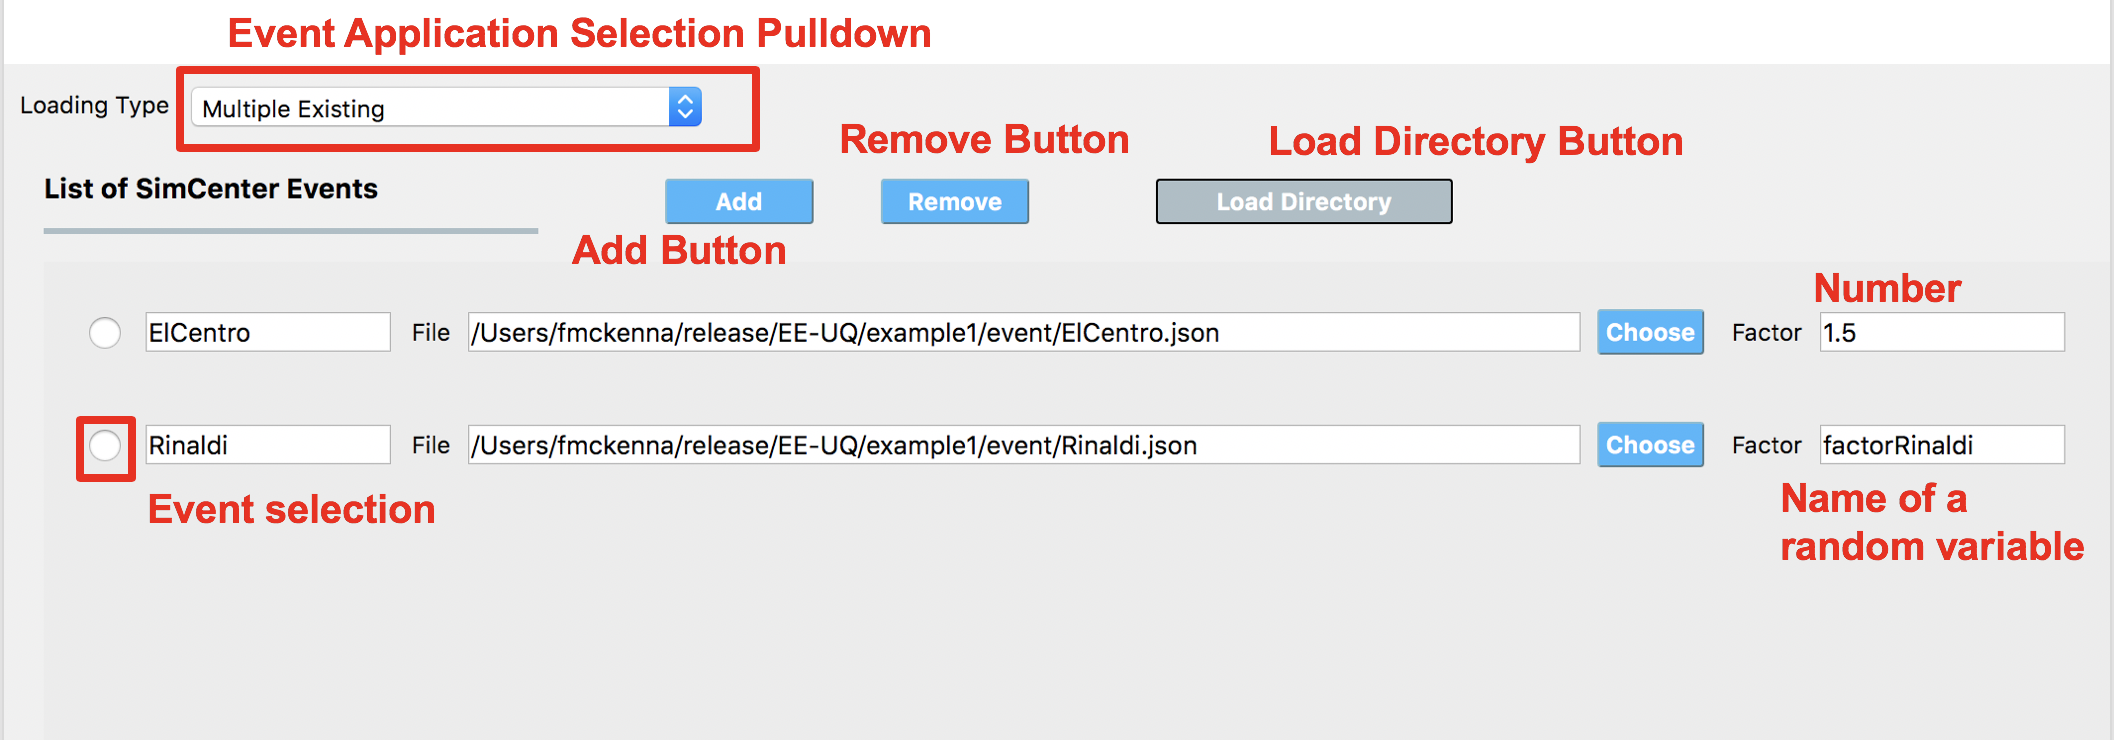
\includegraphics[width=0.8\textwidth]
    {usage/figures/multipleExisting.png} }
  \caption{Multiple Existing (SimCenter) Events }
  \label{fig:SC_event_panel}
\end{figure}

Use the \texttt{Add} button to add a new event. This adds an empty
event to the panel. Pressing the button multiple times will keep
adding events to the panel. \Cref{fig:SC_event_panel} shows the state after
the button has been pressed twice, and data entered to load the El Centro
and Rinaldi Events.

The path to the event file can be entered manually, or using the \texttt{Choose} button for convenience. Pushing the button brings up a typical file search screen. By default, a scale factor of 1.0 is assigned to the event.  The user
can change this to another floating point value (DO NOT USE INTEGER), and they can define the scale factor as a random variable by
entering a variable name, such as \texttt{factorRinaldi} for the second event in \Cref{fig:SC_event_panel}.

Note: the name of the random variable must not start with a number, or contain any spaces or special characters, such as -, +, \%, etc.

The \texttt{Remove} button is used to remove events. To remove an
event, the user must first select events they wish to remove,
which is done by clicking in the small circle at the left side of the event frame. All of the selected events are removed when the \texttt{Remove} button is pressed.

The \texttt{Load Directory} button provides a convenient method to load multiple events. All event files shall first
be placed into the same folder. We recommend to put the files in a folder of their own, with no other files besides the earthquake events in it. After pressing the \texttt{Load Directory} button, the user will be able to choose the directory that contains the files, and the
application will load all event files (i.e., every file with a \texttt{.json} 
extension) into the widget automatically. 

Initially, every
event will be given a load factor of 1.0. Load factors can be assigned automatically by preparing a \texttt{Records.txt} file in the directory with the events. Each line in the \texttt{Records.txt} shall represent one event file, and contain two comma separated values: the event file name and the desired scale factor. The application will open that file automatically and assign the prescribed load factors to the events. Using a \texttt{Records.txt} file also allows users to load only a subset of the events from a folder by listing only those in the file. An example \texttt{Records.txt} is shown below:

\begin{verbatim}
ElCentro.json,1.5
Rinaldi.json,2.0
\end{verbatim}

Random Variables: Scale factors can be defined as being random variables by entering a string in the factor field. The variable name entered will appear as a Random Variable in the UQ panel and the user must specify its distribution there. If multiple
events are specified, the event itself will be also be treated as a random
variable, with each event being part of the discrete set of possible
events. For discrete events the user does not define a distribution, this is done automatically.


\subsection{Multiple PEER Event}
This event option is provided for the user to specify multiple existing
\href{http://peer.berkeley.edu}{PEER} ground
motion files.  For PEER events, the user is required to specify the
individual components for the EVENTS.  The \texttt{Add/Remove} buttons
at the top are to create and remove an event, as
per \Cref{subsec:multiple_existing}. For the PEER events, the user
specifies components acting in the individual degree-of-freedom
directions.  The \texttt{+} and \texttt{-} buttons add and remove
components with remove removing all components selected. Each
component in a PEER event can have their own scale factor, again a
number or a random variable.

\begin{figure}[!htbp]
  \centering {
    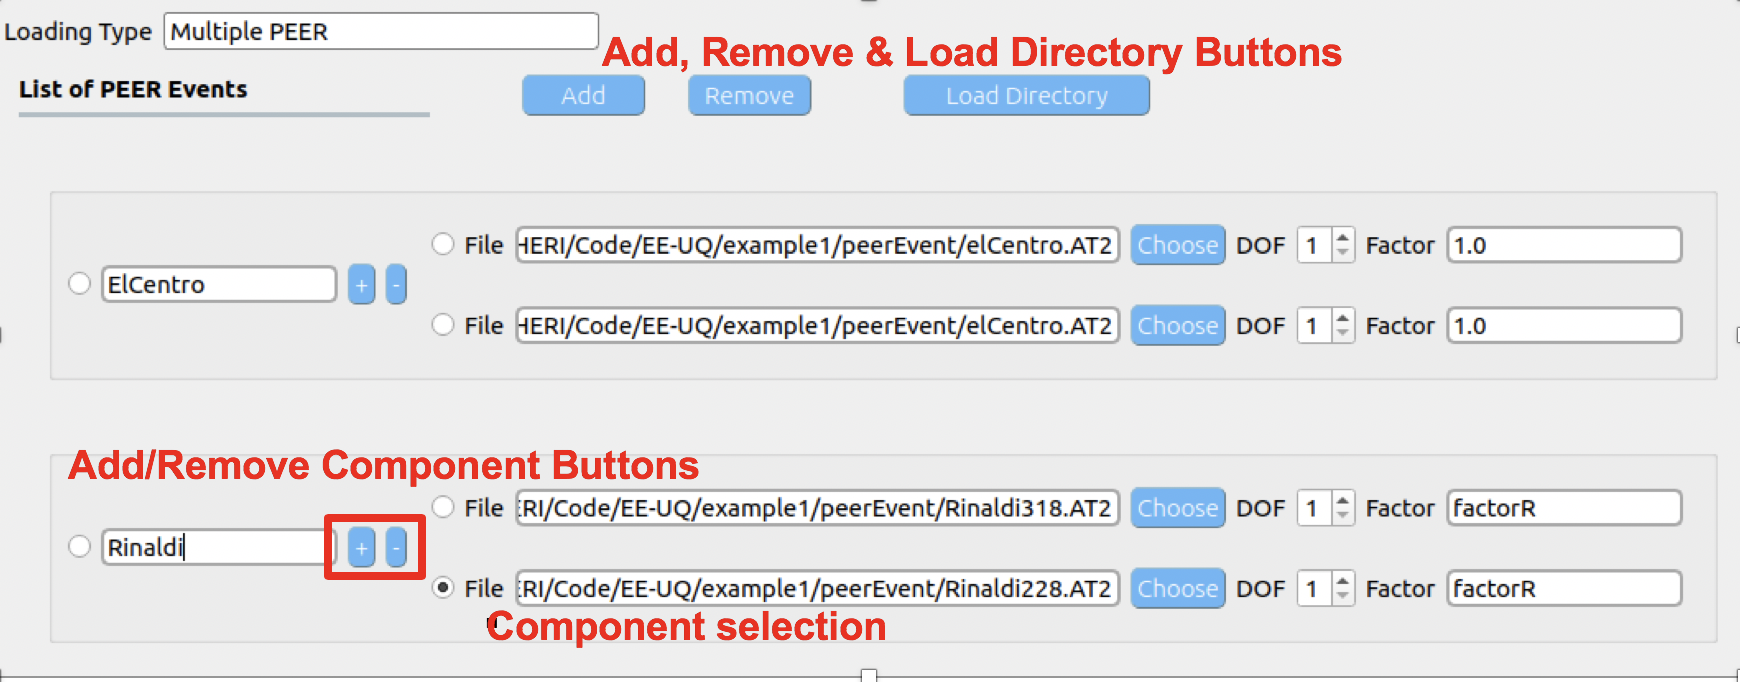
\includegraphics[width=0.8\textwidth]
    {usage/figures/multiplePEER.png} }
  \caption{\texttt{Multiple PEER} loading type}
  \label{fig:figure6}
\end{figure}

If the user has multiple events to load, they can again place all the
PEER \texttt{.AT2} files into a separate folder and select
the \texttt{Load Directory} option. This will allow the user to select
a directory. Once selected, all \texttt{.AT2} files in that directory will be
loaded into the application. Similar to loading multiple SimCenter
events, should the user provide a file \texttt{Records.txt} in that
directory, the application will load all files in the list and set the
appropriate load factor. An example \texttt{Results.txt} file for multiple Peer
events is as shown below:

\begin{verbatim}
elCentro.AT2,1.5
Rinaldi228.AT2,2.0
Rinaldi318.AT2,2.0
\end{verbatim}

Random Variables: The user can, as mentioned, enter a string in the
factor field to specify that the factor is to be considered a random
variable. Subsequently, in the UQ panel the user must provide
information on the random variables distribution. Also, if multiple
events are specified, the event itself will be treated as a random
variable with each event being part of the discrete set of possible
events.


\subsection{Hazard Based Event}
The panel for this event application is as shown in
\autoref{fig:figure7}.  This application implements a scenario-based
(deterministic) seismic event.  In this panel the user specifies an
earthquake rupture (location, geometry and magnitude), a ground motion
prediction equation, a record selection database and the intensity
measure used for record selection.  In the backend, this application
relies on three other applications to perform seismic hazard analysis,
intensity measures simulation (to create a simulated target spectrum),
and ground motion record selection/scaling.  Users interested in
learning about those applications are referred to the documentation of
the
(\href{https://github.com/NHERI-SimCenter/GroundMotionUtilities/blob/master/Readme.md}{SimCenter
  ground motion utilities}).

\begin{figure}[!htbp]
  \centering {
    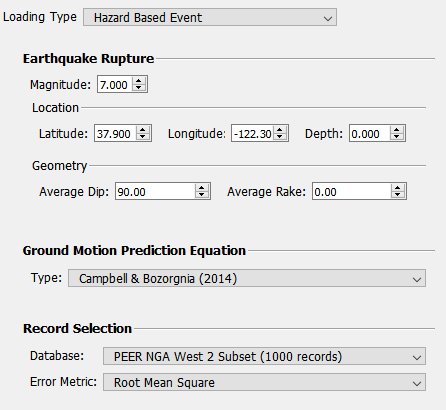
\includegraphics[width=0.8\textwidth]
    {usage/figures/hazardBased.png} }
  \caption{\texttt{Hazard Based Event} loading type}
  \label{fig:figure7}
\end{figure}


\subsection{Stochastic Ground Motion Model}
This option allows users to generate synthetic ground motions for a
target seismic event. In order to do so, the stochastic ground motion
model is selected from the drop-down menu, as shown
in \Cref{fig:stochastic_loading}. Depending on the model selected, the
user will be asked to enter values for a number of parameters that are
used to generate a seismic event. In the current release, users can
select between the model derived by Vlachos et
al. (2018) \cite{vlachos2018predictive} and the model developed by
Dabaghi \& Der Kiureghian (2014, 2017, 2018)
[\cite{dabaghi2014stochastic}, \cite{dabaghi2017stochastic}, \cite{dabaghi2018simulation}]. Additionally,
users can provide a seed for the stochastic motion generation if they
desire the same suite of synthetic motions to be generated on multiple
occasions.  If the seed is not specified, a different realization of
the time history will be generated for each run. The backend
application that generates the stochastic ground motions relies
on \texttt{smelt}, a modular and extensible C++ library for generating
stochastic time histories. Users interested in learning more about the
implementation and design of
\texttt{smelt} are referred to its
\href{https://github.com/NHERI-SimCenter/smelt}{GitHub repository}.

All input parameters can be specified as random variables by entering
a string in the parameter field. Please note that information for the
inputs that are identified as random variables needs to be provided in
the \texttt{UQ} tab.

\begin{figure}[!htbp]
  \centering {
    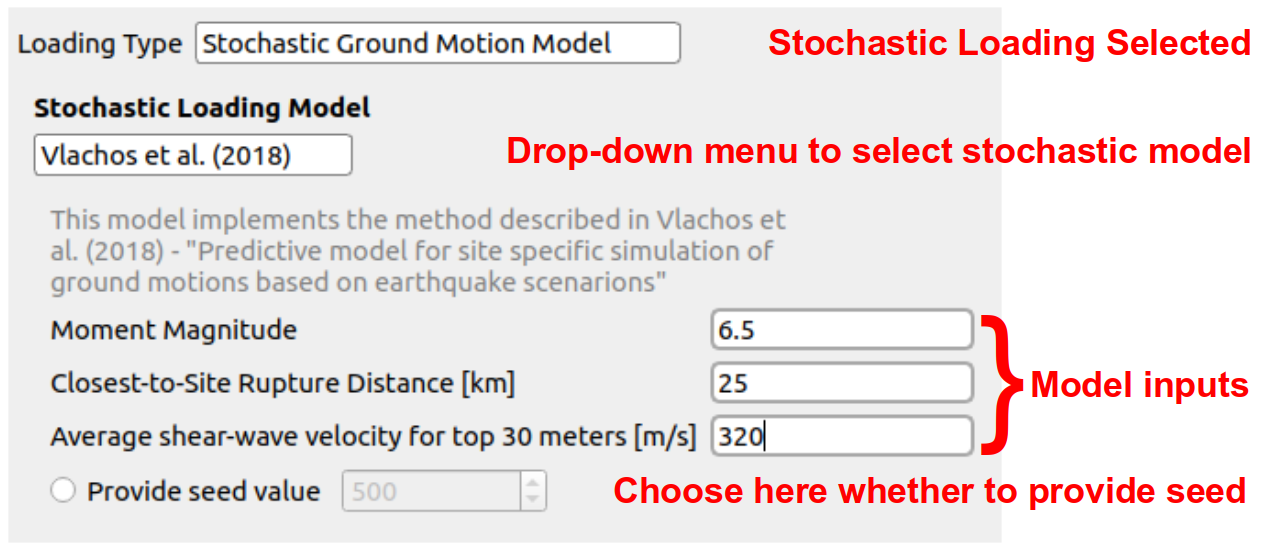
\includegraphics[width=0.8\textwidth]
    {usage/figures/stochastic_loading.png} }
  \caption{Stochastic Ground Motion Event}
  \label{fig:stochastic_loading}
\end{figure}


\subsection{Site Response}
The panel for this event application is as shown in \Cref{fig:s3hark0}. 
This application does effective free-field site response analysis of a soil column.
In this panel the user specifies a ground motion at the bottom of the column. 
With soil layer properly defined, the motion at the ground surface will be given at the end of the analysis.
\begin{figure}[!htbp]
  \centering {
    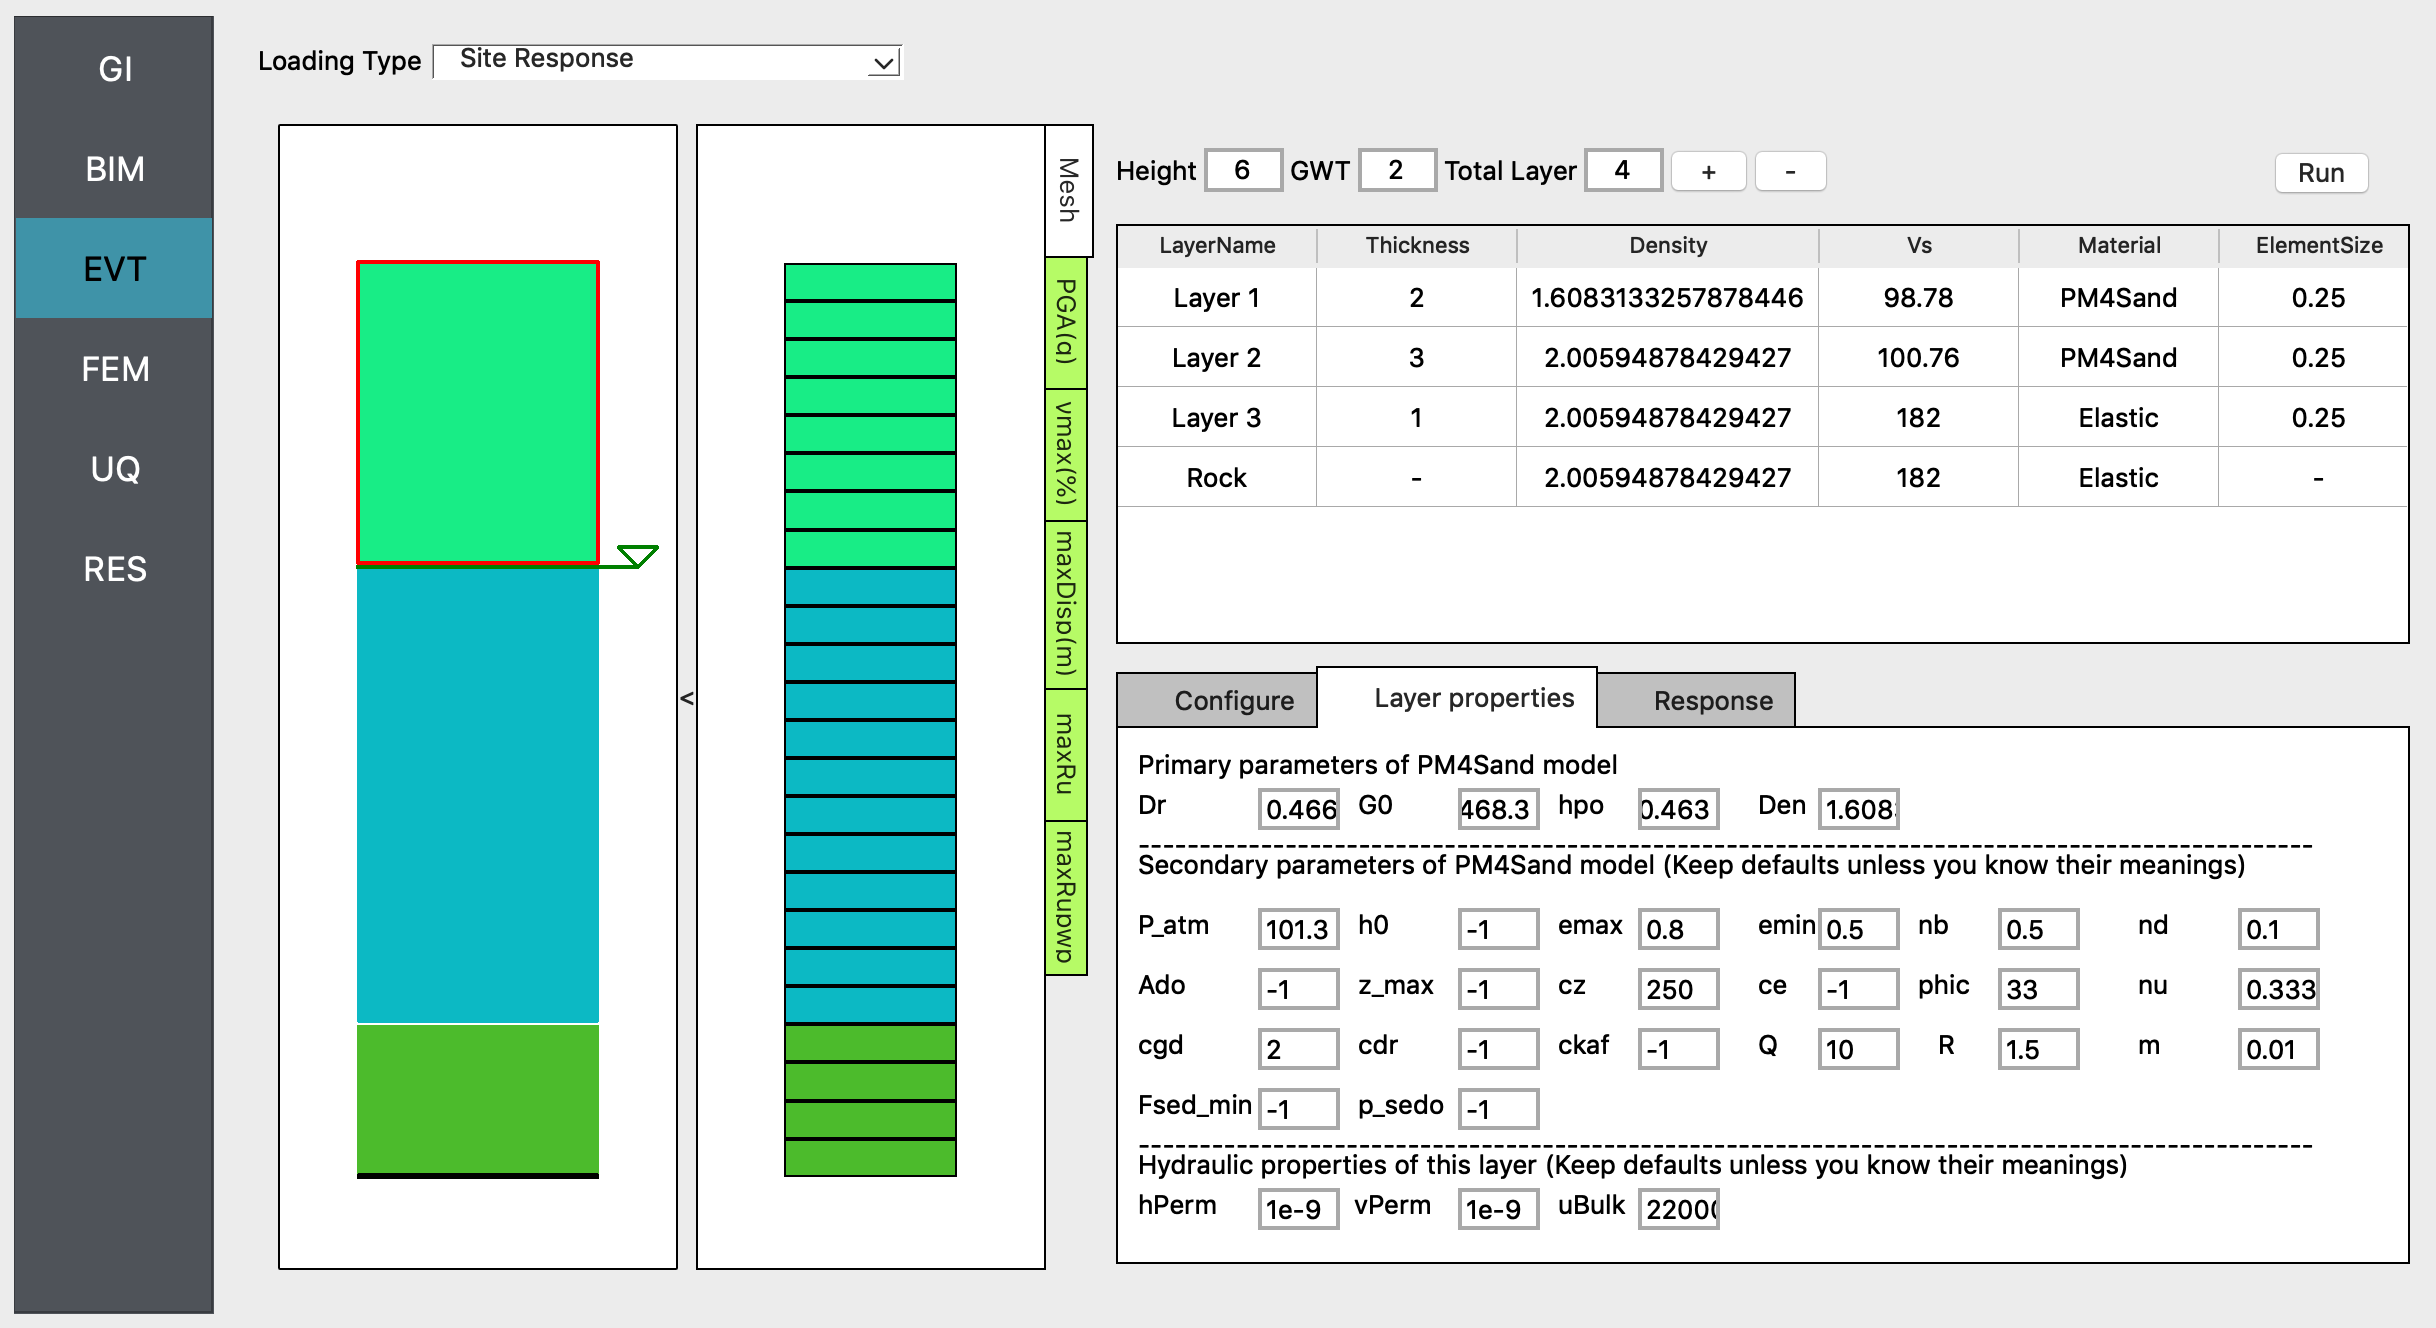
\includegraphics[width=0.8\textwidth]
    {usage/figures/s3hark0.png} }
  \caption{s$^3$hark}
  \label{fig:s3hark0}
\end{figure}

The UI of s$^3$hark is shown in \Cref{fig:s3hark1}.
There are two graphics shown in the left of the panel. The first one is the soil column graphic, 
which shows a visualization of the soil column.
The second one is the mesh and profile graphic, 
which shows the finite element mesh and profile plots.
On the right of the panel are operation area, soil design table, configure tab, layer property tab and response tab. 


\begin{figure}[!htbp]
  \centering {
    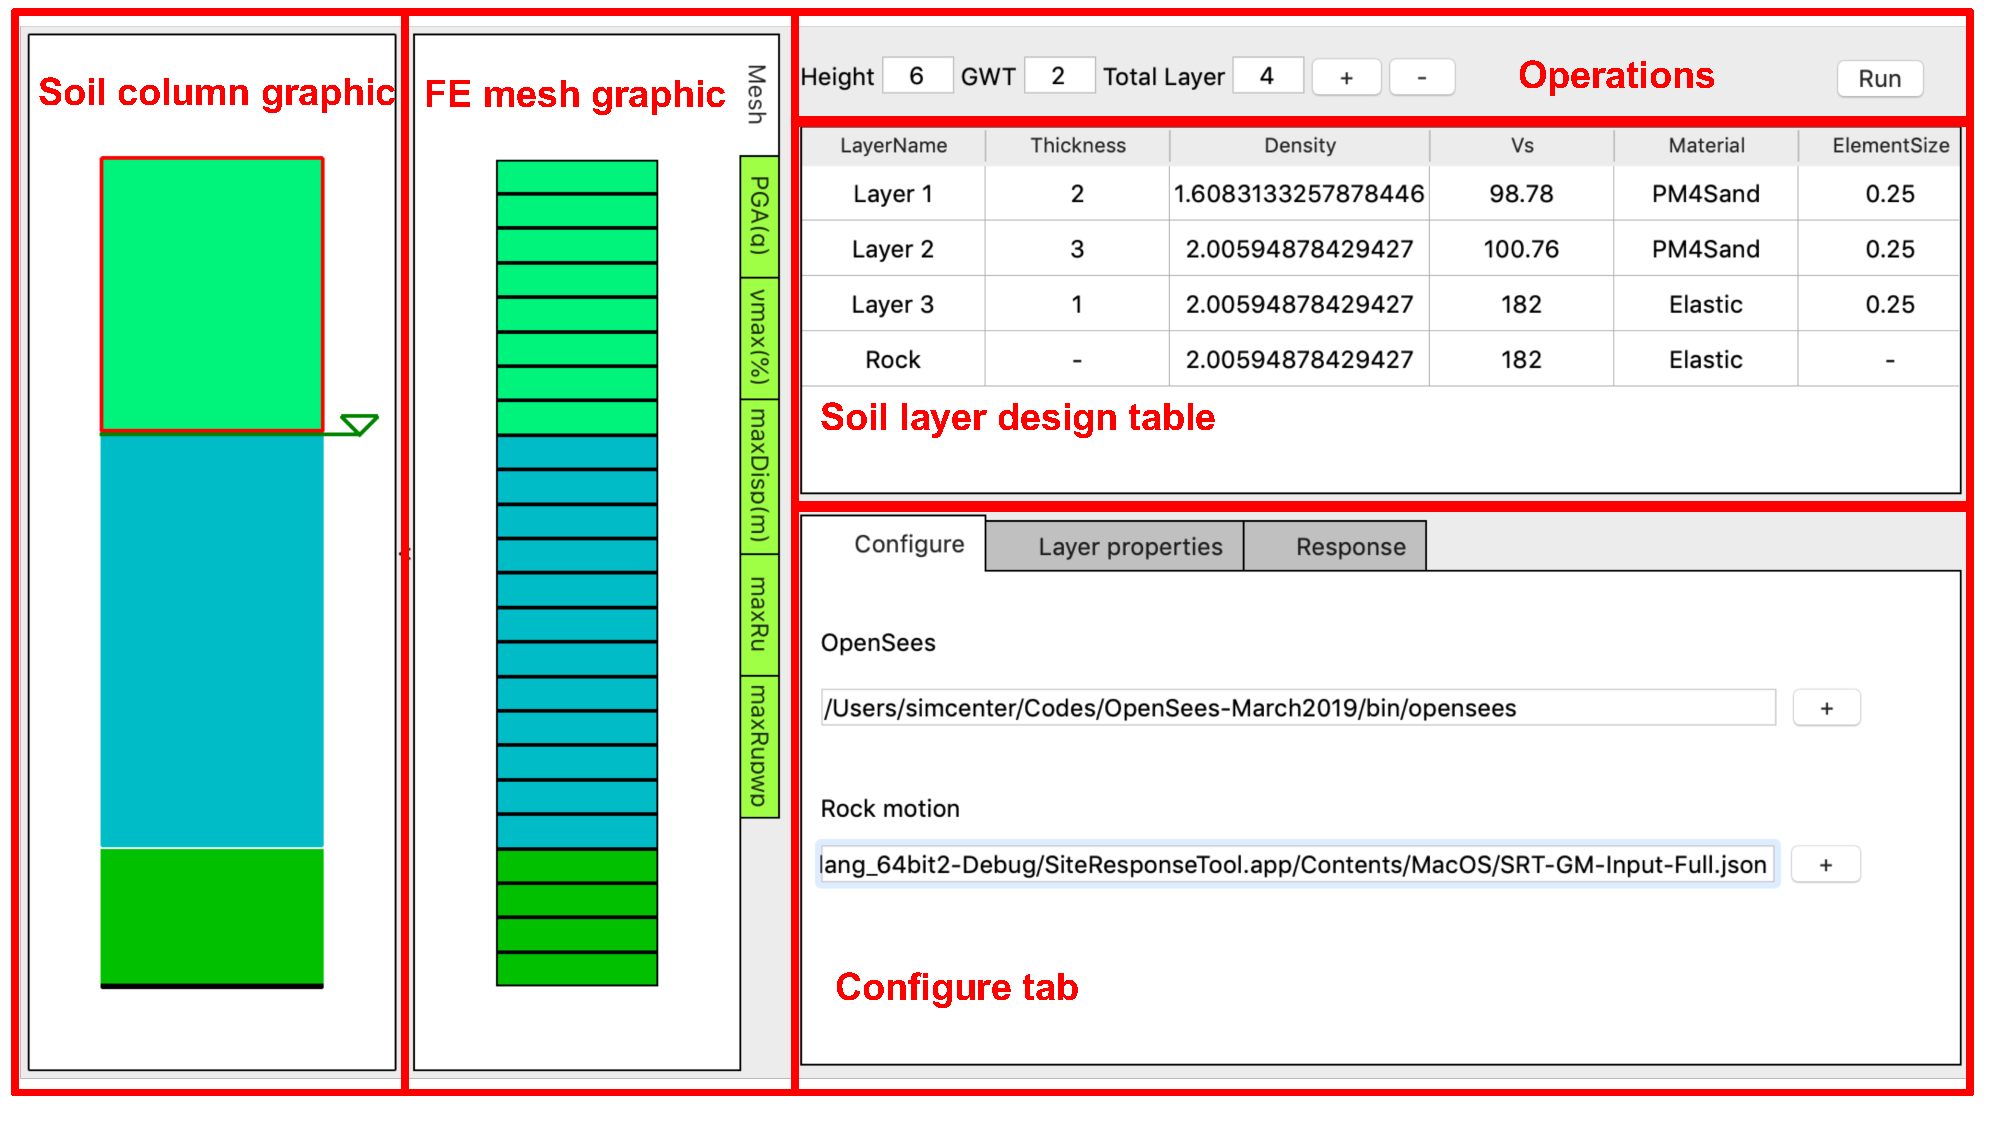
\includegraphics[width=0.8\textwidth]
    {usage/figures/s3hark1.pdf} }
  \caption{s$^3$hark - Panels}
  \label{fig:s3hark1}
\end{figure}

In the operation area as shown in \Cref{fig:s3hark2}, click the plus button to add a layer and the minors button to delete a selected layer. 
Change the ground water table in the GWT input field. 
In the configure tab, path of OpenSees executable and rock motion file need to be specified.
A click on the run button will start the finite element analysis.


\begin{figure}[!htbp]
  \centering {
    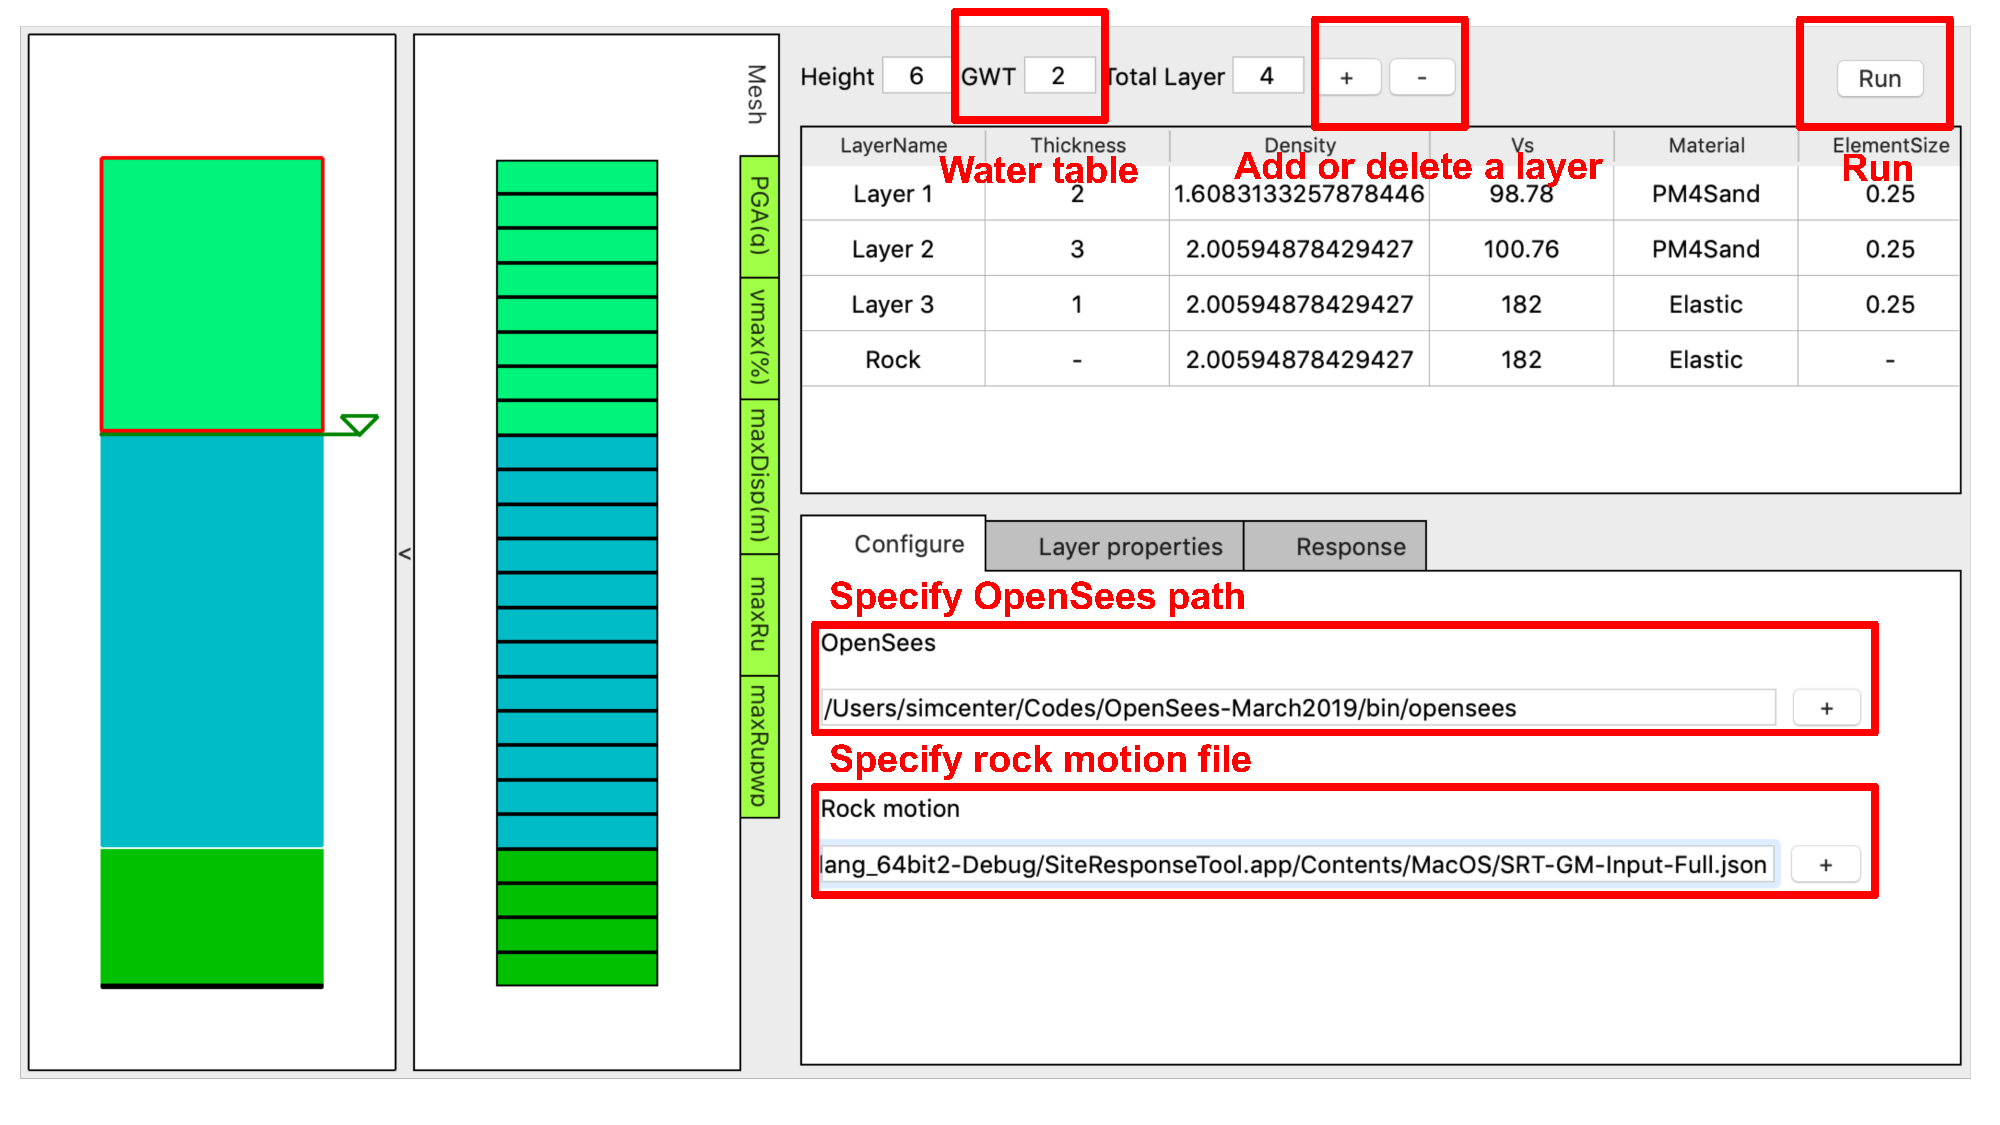
\includegraphics[width=0.8\textwidth]
    {usage/figures/s3hark2.pdf} }
  \caption{s$^3$hark - Configurations and Operations }
  \label{fig:s3hark2}
\end{figure}

Either click on the soil column or the table to select a layer \Cref{fig:s3hark3}. 
When a layer is selected, it will be highlighted in both the soil column graphic and the table. 
Selection of a soil layer will invoke the Layer properties tab, where the user can specify the material properties of this layer.
Double click on a cell of the table will allow the user to change the corresponding value.

\begin{figure}[!htbp]
  \centering {
    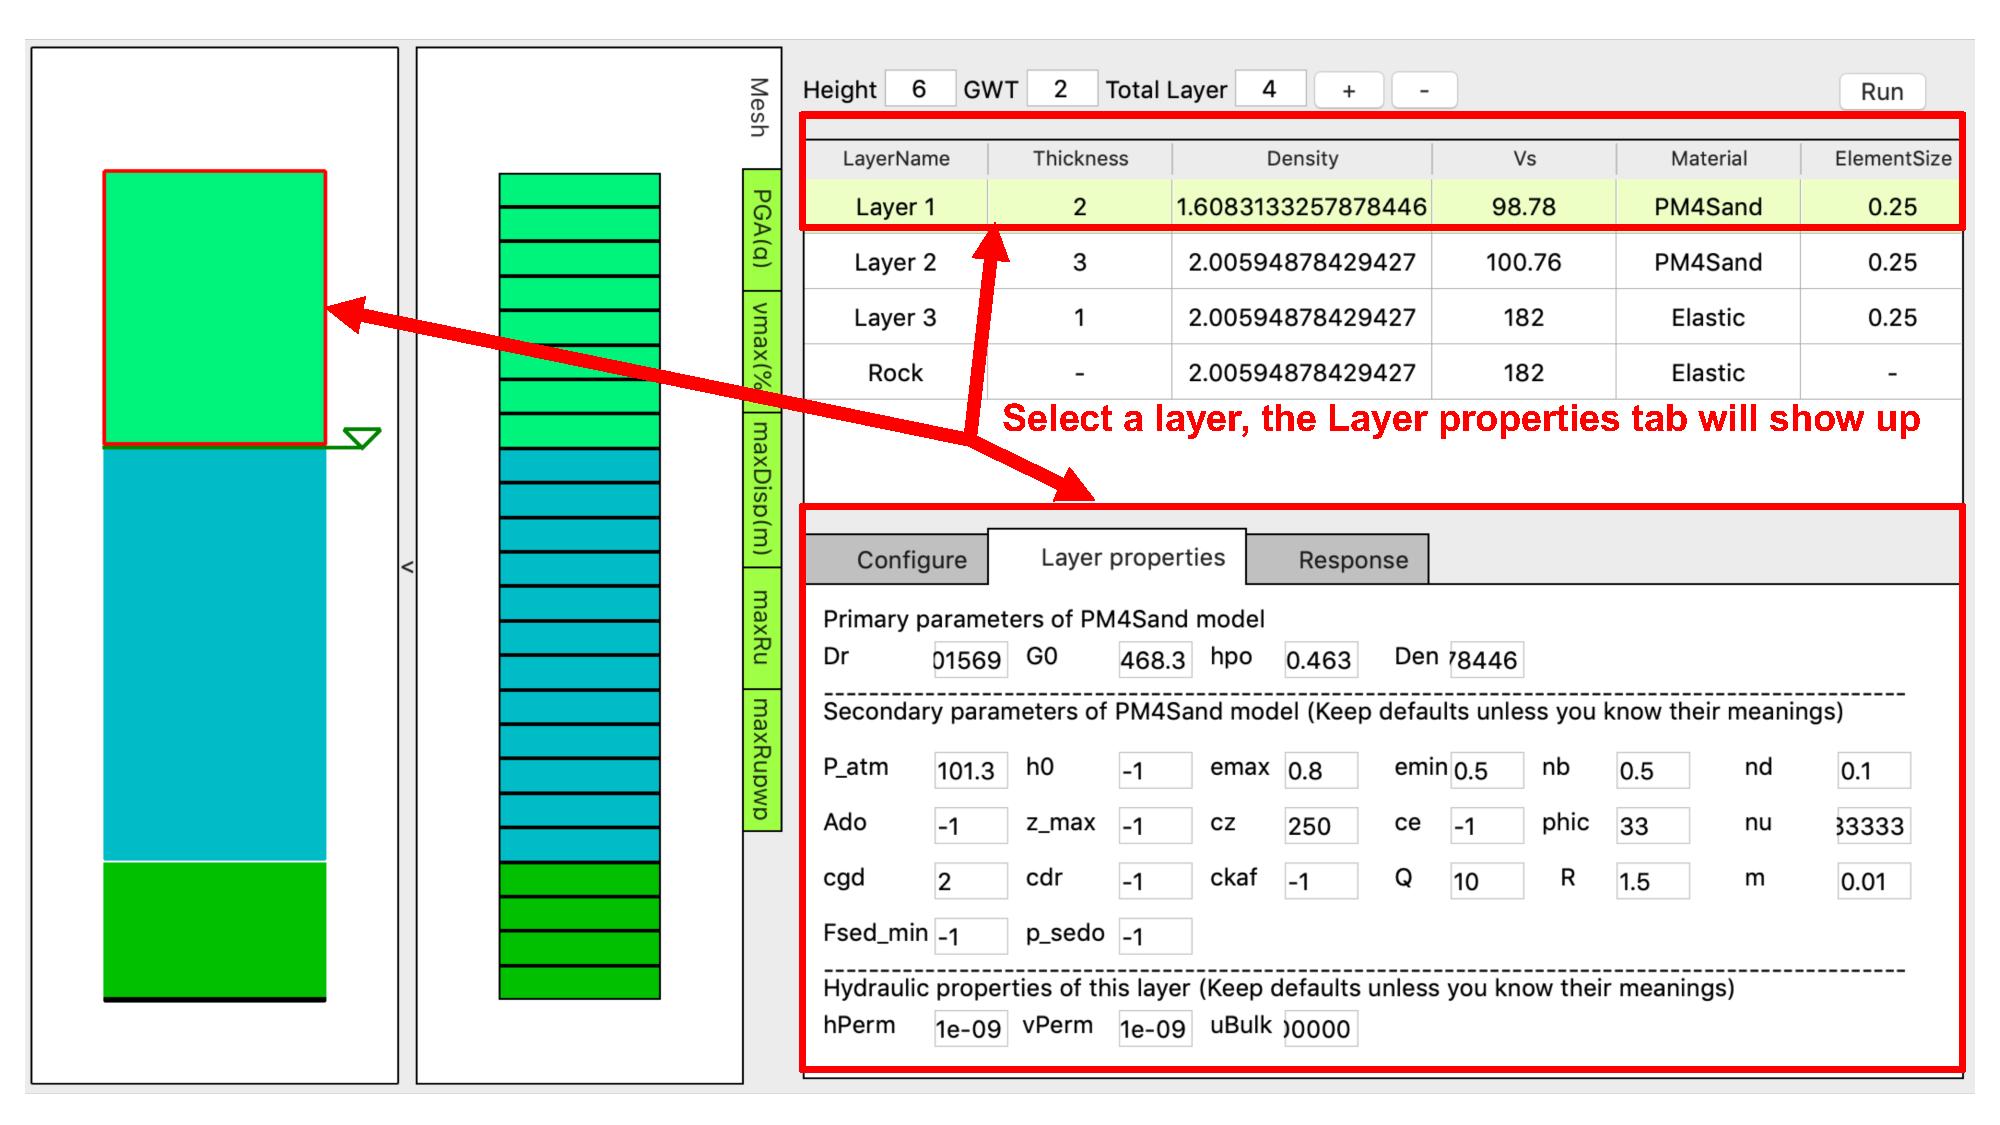
\includegraphics[width=0.8\textwidth]
    {usage/figures/s3hark3.pdf} }
  \caption{s$^3$hark - Layer modification }
  \label{fig:s3hark3}
\end{figure}


Upon the finish of the finite element analysis, the ground motion at the soil surface (\Cref{fig:s3hark4}) will be stored in EE-UQ's input file.
This computed motion will be later applied to the bottom of the building.

\begin{figure}[!htbp]
  \centering {
    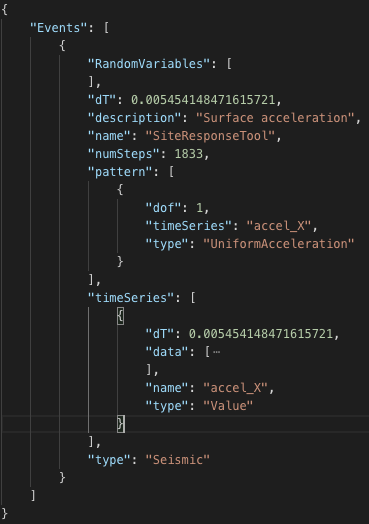
\includegraphics[width=0.4\textwidth]
    {usage/figures/s3hark4.png} }
  \caption{s$^3$hark - Surface motion }
  \label{fig:s3hark4}
\end{figure}


\subsection{User Application}
The final option for event definition is a user application. 
The user specifies the application name and the input file containing the specific input information 
needed by the application when it is running in the backend. 
As will be discussed later, when they use an additional application not provided, the user is also required 
to edit the tools registry file. There they must include a new event application with the same name 
and the location where that application can be found relative to the tools application directory. 
If running on DesignSafe, that application must be built and must be available on the Stampede2 supercomputer. 

Note: Given how DesignSafe runs the applications through Agave, the file permissions of this application must be 
world readable and executable (i.e., when a user runs their application through DesignSafe and Agave, they are not running it as themselves!)

\begin{figure}[!htbp]
  \centering {
    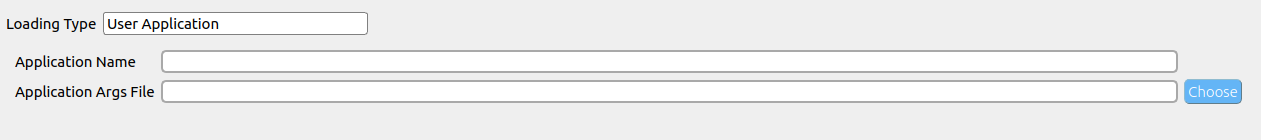
\includegraphics[width=1.0\textwidth]
    {usage/figures/userAppEvent.png} }
  \caption{User defined event}
  \label{fig:user_defined_event_panel}
\end{figure}



\section{FEM: Finite Element Method}
The FEM panel is intended to present users with a selection of FEM
applications that will take a building model generated by the BIM
application and the EVENT from the event application and perform a
deterministic simulation.  At present there is only one application
available, OpenSees and there is no application selection box.  That
will be modified in future versionsto allow user to provide their own
simulation application.  This is not the standard OpenSees executable,
but consists of a pre- and post-processor to take the BIM and EVENT
file and use OpenSees to determine the response, returning these
responses in an EDP.

For the OpenSees application the user is required to specify the
options to be used in the transient analysis. As shown \autoref{fig:fem},
this includes the choice of
\begin{enumerate}
\item Solution algorithm, the default is Newton Raphson.
\item Integration Scheme, the default is Newmarks linear acceleration
  method.
\item Convergence Test, the default is a norm on the unbalance force.
\item Convergence tolerance
\item Damping Ratio.
\end{enumerate}

\begin{figure}[!htbp]
  \centering {
    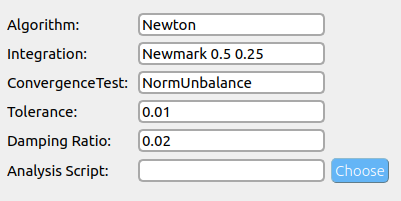
\includegraphics[width=0.8\textwidth]
    {usage/figures/fem.png} }
  \caption{Options for \texttt{OpenSees} transient analysis}
  \label{fig:fem}
\end{figure}

All the options available can be found in the OpenSees online user
manual.\\

A default transient analysis script is run with these inputs. It is
built for Version 3.0.0+ of OpenSees and uses a divide and conquer
algorithm in event of a convergence failure issue. This new algorithm
does not always work. \\

The user is also able to specify their own analysis script to run
instead of the default. When chosen the variables numStep and dt that
are obtained from the EVENT are set by the program. These variables
can be used by the user when providing their own analysis script.


\section{UQ: Uncertainty Quantification}
Throughout the input specification the user is defining variables. As
described in the above sections many of these variables can be
specified by the user to be random variables. The UQ panel is where the user specifies the distribution of these random variables. Besides the properties of random variables, the sampling method and the number of requested samples shall also be defined by the user. The panel is split, as shown
in \Cref{fig:uq_panel}, into two frames:

\begin{enumerate}
\item Sampling Methods 
\item Random Variables
\end{enumerate}

\begin{figure}[!htbp]
  \centering {
    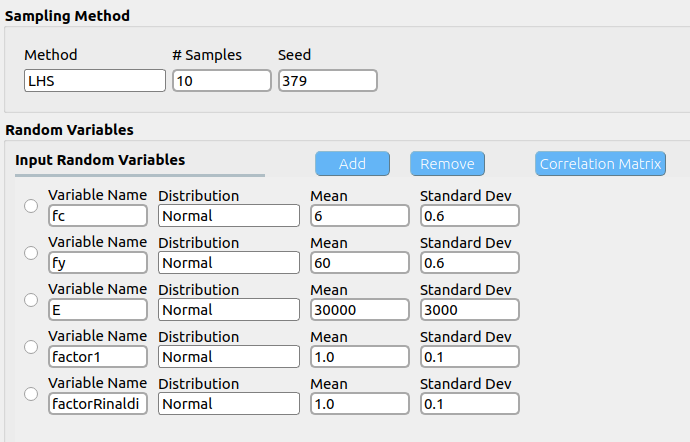
\includegraphics[width=0.8\textwidth]
    {usage/figures/uq1.png} }
  \caption{Uncertainty Quantification input panel}
  \label{fig:uq_panel}
\end{figure}

\subsection{Sampling Methods}
In the forward propagation problem, the user selects the sampling 
method to use from the dropdown menu \href{https://dakota.sandia.gov//sites/default/files/docs/6.9/html-ref/method-sampling.html}{sampling methods}. Currently there are five options available: 
Monte Carlo Sampling (MCS),  Latin Hypercube Sampling (LHS), Importance Sampling (IS), and sampling based on surrogate models, including Gaussian Process Regression (GPR) and Polynomial Chaos Expansion (PCE). Depending on the option selected, the user must specifies the appropriate input parameters for each. For instance, for MCS, the number of samples specifies the number of simulations to be performed, and providing a random seed allows the user to reproduce the same set of samples from the random variables multiple times.

\begin{figure}[!htbp]
  \centering {
    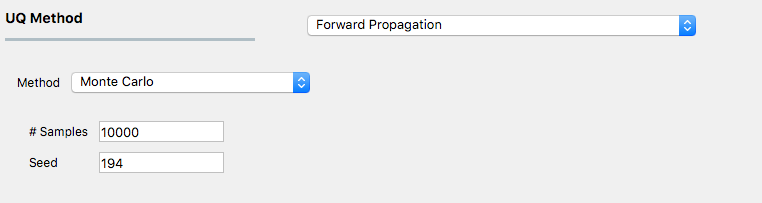
\includegraphics[width=1.0\textwidth]
    {examples/fig_quofem/fw_mc.png} }
  \caption{Monte Carlo Sampling input panel}
  \label{fig:mcs}
\end{figure}

Figure \Cref{fig:mcs} shows the input panel corresponding to the Monte Carlo Sampling (MCS) setting. Two input parameters need to be specified, the number of samples to be executed, as well as the seed used in generating the random samples. 


\begin{figure}[!htbp]
  \centering {
    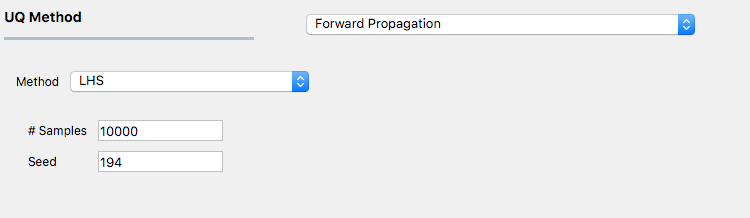
\includegraphics[width=1.0\textwidth]
    {examples/fig_quofem/fw_lhs.png} }
  \caption{Latin Hypercube Sampling input panel}
  \label{fig:lhs}
\end{figure}

Figure \Cref{fig:lhs} shows the input panel corresponding to the Latin Hypercube Sampling (LHS) scheme. Two input parameters also need to be specified, the number of samples to be executed, as well as the seed used in generating the LHS samples. 

\begin{figure}[!htbp]
  \centering {
    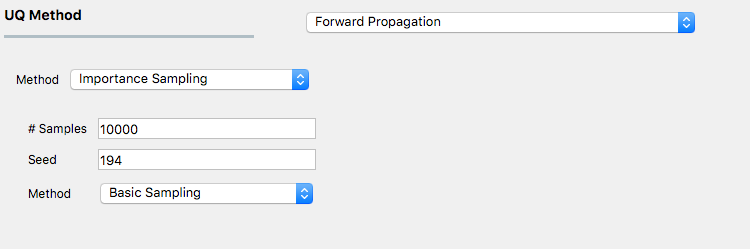
\includegraphics[width=1.0\textwidth]
    {examples/fig_quofem/fw_is.png} }
  \caption{Importance Sampling input panel}
  \label{fig:is}
\end{figure}

For rare event analysis, Figure \Cref{fig:is} shows the input panel for Importance Sampling (IS) scheme. Similar to MCS and LHS, the IS requires both the number of samples to be executed and the corresponding seed for generating such random samples. In addition, the Importance Sampling algorithm can performed via three different approaches, as specified by the third input method. The latter includes Basic Sampling, Adaptive Sampling, and Multimodal Adaptive Sampling. 


For uncertainty propagation with surrogates, two popular surrogates are available, namely Gaussian Process Regression (GPR) and Polynomial Chaos Expansion (PCE). Figure \Cref{fig:gpr} shows the input panel for the GPR model, with input panels for training and sampling. 

\begin{figure}[!htbp]
  \centering {
    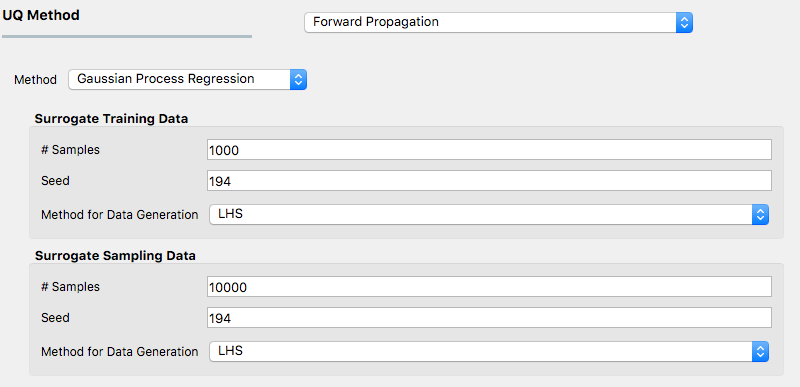
\includegraphics[width=1.0\textwidth]
    {examples/fig_quofem/fw_gp.png} }
  \caption{GPR forward propagation input panel}
  \label{fig:gpr}
\end{figure}

For uncertainty propagation with Gaussian Process Regression (GPR), Figure \Cref{fig:gpr} shows the input panel for the PCE model, with input panels for training and sampling as well. The first set of input parameters in the surrogate training data specify the dataset used for training the surrogate model, while the second set of input parameters in the surrogate sampling data relate to the dataset used for sampling the surrogate. Care must be taken in specifying the training dataset to results in an accurate response surface approximation. 

\begin{figure}[!htbp]
  \centering {
    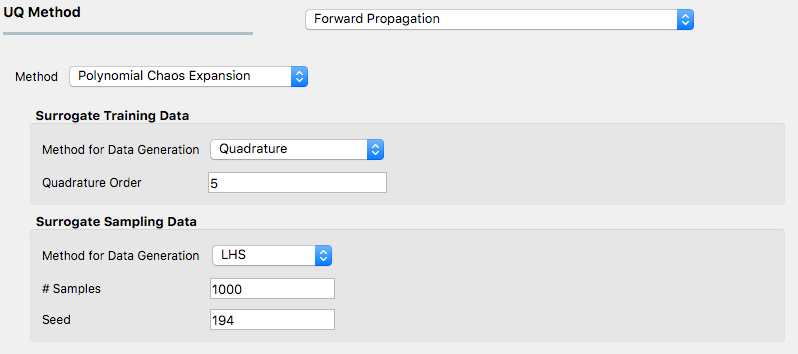
\includegraphics[width=1.0\textwidth]
    {examples/fig_quofem/fw_pce.png} }
  \caption{PCE forward propagation input panel}
  \label{fig:pce}
\end{figure}

For uncertainty propagation with Polynomial Chaos Expansion (PCE), Figure \Cref{fig:pce} shows the input panel for the PCE model, with input panels for training and sampling as well, similar to the input GPR panel. The first set of input parameters in the surrogate training data specify the dataset used for training the surrogate model, while the second set of input parameters in the surrogate sampling data relate to the dataset used for sampling the surrogate. Extreme care must be taken in specifying the parameters of the training dataset to results in an accurate response surface approximation. 

If you are not sure about the training parameters of the surrogates, please refrain from using the surrogates for forward propagation and use instead conventional sampling such as MCS and LHS as discussed above. 

\subsection{Reliability Analysis}

For reliability analysis, figure \Cref{fig:rel} shows the input panel for the reliability capabilities. Currently, both First-Order Reliability Methods (FORM) and Second-Order Reliability Methods (SORM) are supported. The user can specify the local or global solution in the Reliability Scheme input parameter. In addition, the user needs to specify the method for searching for the Most Probable Point (MPP); if not sure, do not use any MPP approximation. 

For both first and second-order reliability analysis, the user needs to specify the either the response levels or the probability levels at which the CDF of the QoI needs to be queried. The user can specify multiple query points, separated by a space. 


\begin{figure}[!htbp]
  \centering {
    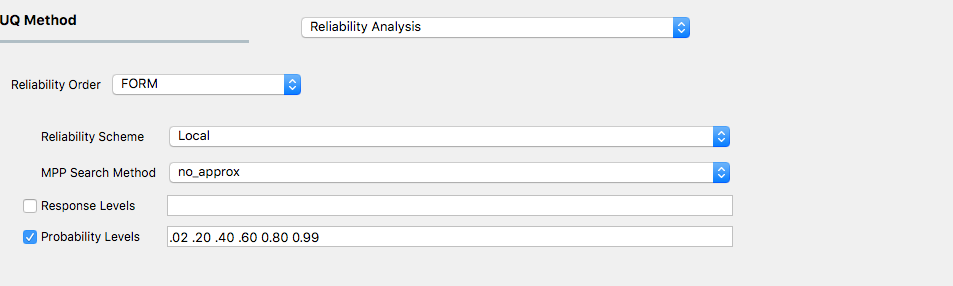
\includegraphics[width=1.0\textwidth]
    {examples/fig_quofem/rel_form.png} }
  \caption{Reliability input panel}
  \label{fig:rel}
\end{figure}




\subsection{Random Variables}
The RV panel allows the user to specify the probabilistic distribution for the random problem at hand. The following probabilistic distributions for the random variables are currently supported: 
\begin{enumerate}
\item Gaussian
\item Lognormal
\item Beta
\item Uniform
\item Weibull
\item Gumbell
\end{enumerate}

Each distribution has different parameters, and the user needs to select accordingly the parameters for the distribution selected for each random variable. Once the user selects the distribution of the random variable, the
corresponding input boxes for the parameters will show. 

\Cref{fig:rv} shows the panel for a problem with four Random Variables with all random input following Gaussian distributions. 

\begin{figure}[!htbp]
  \centering {
    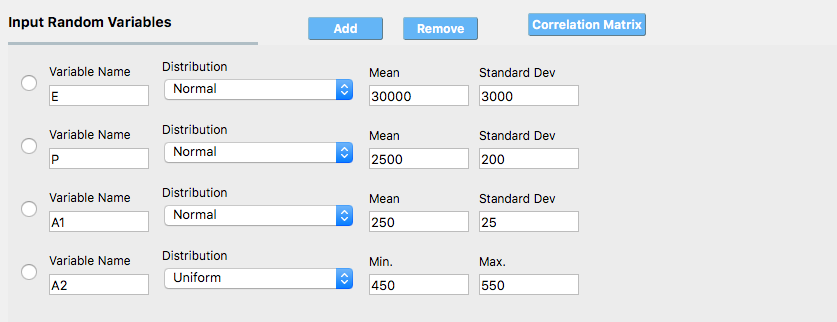
\includegraphics[width=0.8\textwidth]
    {examples/fig_quofem/rv.png} }
  \caption{Random Variable specification}
  \label{fig:rv}
\end{figure}





\section{EDP: Engineering Demand Parameters}
This panel is where the user selects which outputs will be displayed when
the simulation runs. There are two options available in the pull-down
menu:
\begin{enumerate}
  \softwareSwitch{WE-UQ}{
    \item Standard Wind (\Cref{subsec:sectionStandardWind})    
  }{
    \item Standard Earthquake (\Cref{subsec:sectionStandardEarthquake})    
  }
\item User Defined (\Cref{subsec:sectionUserDefined})
\end{enumerate}

\softwareSwitch{WE-UQ}{
  \subsection{Standard Wind}\label{subsec:sectionStandardWind}
  When the user selects Standard Wind there are no additional
  inputs required. The standard wind EDP generator will ensure the
  the max absolute value of the following are obtained:  
}{
  \subsection{Standard Earthquake}\label{subsec:sectionStandardEarthquake}
  When the user selects Standard Earthquake there are no additional
  inputs required. The standard earthquake EDP generator will ensure the
  the max absolute value of the following are obtained:  
}
\begin{enumerate}
\item Relative Floor displacements:
\item Absolute Floor Accelerations
\item Interstory Drifts
\end{enumerate}

The results will contain results for these in abbreviated form:
\begin{itemize}
\item PFD peak relative floor displacement $1-PFD-FLOOR_CLINE$
\item PFA peak floor acceleration (relative + ground motion):
  $1-PFA-FLOOR-CLINE$
\item PID peak inter-story drift: $1-PID-STORY-CLINE$
\end{itemize}

NOTE: Floors are numbered starting at floor 0, and stories are numbered starting at story 1.

\subsection{User Defined}\label{subsec:sectionUserDefined}
As shown in \Cref{fig:userEDP}, this panel allows the user to determine their own output and process it. When using this option the user provides additional data:

\begin{figure}[!htbp]
  \centering {
    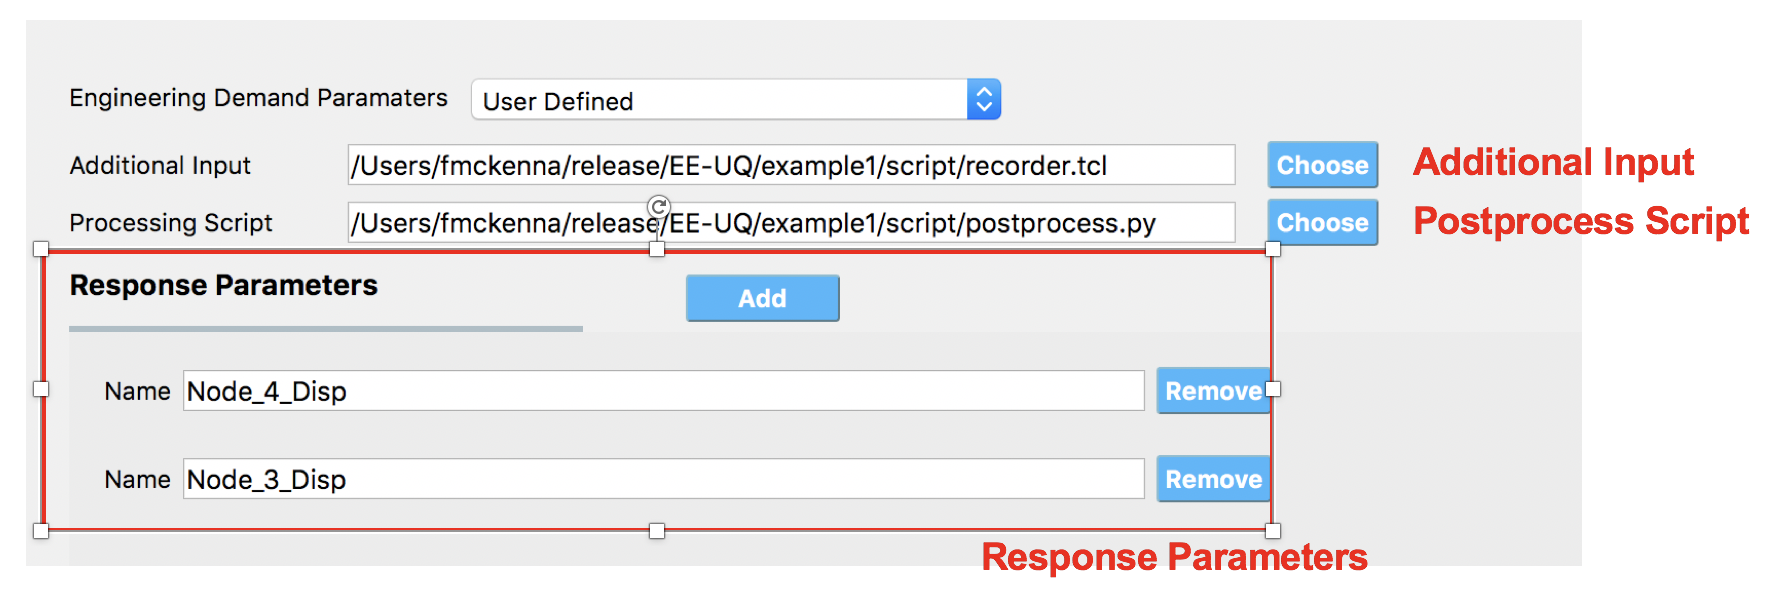
\includegraphics[width=0.8\textwidth]
    {usage/figures/userDefinedEDP.png} }
  \caption{userEDP}
  \label{fig:userEDP}
\end{figure}

\begin{enumerate}
\item Additional Input: These are additional commands that are invoked
  by the analysis application before the transient analysis is
  performed. For example, for OpenSees this would be a script
  containing a series of recorder commands. \\

A recorder file passed to OpenSees might look like the following:
\begin{verbatim}
recorder EnvelopeNode -file node.out -node 1 2 3 4 -dof 1 disp
recorder EnvelopeElement -file ele.out -ele 1 2 3 forces
\end{verbatim}

\item Postprocess Script: This is a python script that will be invoked
  after the finite element application has run. It must be provided by
  the user. It's purpose is to process the output files and create a
  single file, results.out. This file must contain a single line with
  as many entries as EDP's specified.

For example, a postprocessing file that would take the outputs from the analysis to create the results file might look like the following:

\begin{python}
#!/usr/bin/python                                                                 

import sys
import re

EDPs = ['Node_4_Disp', 'Node_3_Disp']

inputArgs = sys.argv

with open ('node.out', 'rt') as inFile:
    line = inFile.readline()
    line = inFile.readline()
    line = inFile.readline()
    displ = line.split()
    numNode = len(displ)

inFile.close

#                                                                                 
# now process the input args and write the results file                           
#                                                                                 

outFile = open('results.out','w')

#                                                                                 
# note for now assuming no ERROR in user data                                     
#                                                                                 

for i in EDPs[0:]:
    print i
    theList=i.split('_')

    if (theList[0] == 'Node'):
        nodeTag = int(theList[1])

        if (nodeTag > 0 and nodeTag <= numNode):
            if (theList[2] == 'Disp'):
                nodeDisp = displ[nodeTag-1]
                outFile.write(nodeDisp)
                outFile.write(' ')
            else:
                outFile.write('0. ')
        else:
            outFile.write('0. ')
    else:
        outFile.write('0. ')

outFile.close
\end{python}



\item Response Parameters. This is an area in which the user
  associates a variable name with the column of the results output
  file. If the process script has an array of strings named named
  EDP's the script, the Response Parameters will be initially set with
  these values from the script.
\end{enumerate}



\section{RES}
When the user hits the Run button, and assuming the results are
successful. The results are presented here.  A successful run or
download of a job that ran successfully will result in 3 tabbed
widgets being displayed in this panel.  The first panel shows summary
statistics: mean and stdDev values or min-max values if discrete set,
i.e. multiple events for each of the EDP's specified in the EDP panel.

\begin{figure}[!htbp]
  \centering {
    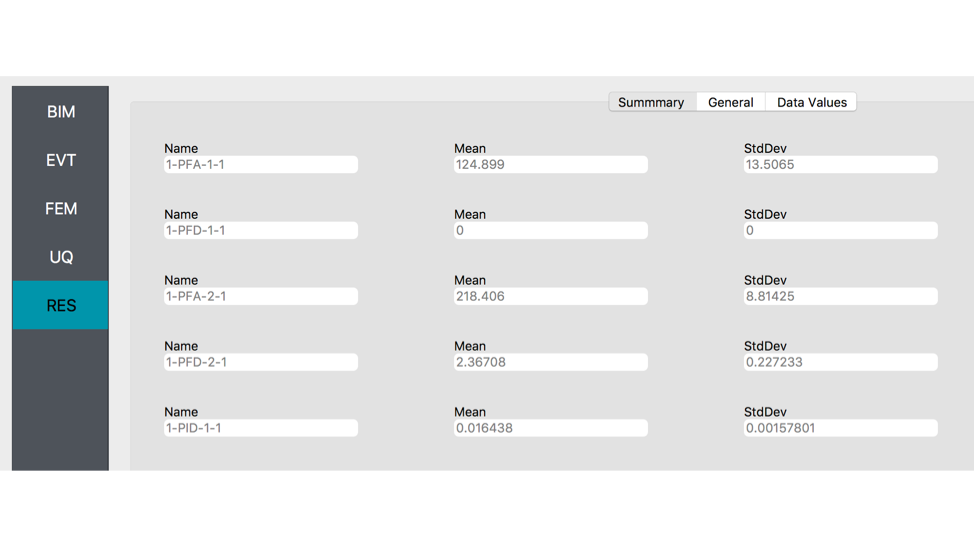
\includegraphics[width=0.8\textwidth]
    {figs/Figure12.png} }
  \caption{RES}
  \label{fig:figure12}
\end{figure}

The second panel shows the summary information.

\begin{figure}[!htbp]
  \centering {
    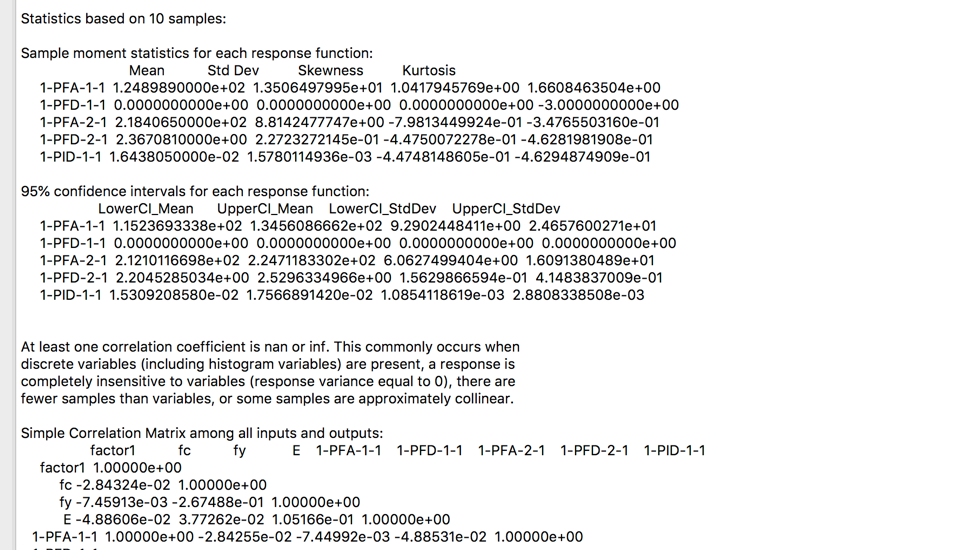
\includegraphics[width=0.8\textwidth]
    {figs/Figure13.png} }
  \caption{RES General tab}
  \label{fig:figure13}
\end{figure}

The third panel presents graphically and in tabular form the
results. By selecting different columns with left and right mouse
buttons in the table below the graphic, the information in the graph
is changed. Selecting the left mouse button changes the Y axis, the
right mouse changes the X axis. If the same column is selected using
both left and right keys, the CDF and PDF is displayed. If last mouse
press was with the left button, the PDF and if right the CDF.
 
As for the columns. You will see a column for each random variable the
workflow came across. There may be more than you specified if the
applications want the UQ engine to consider their own variables in the
computation. The outputs at present are limited to:

\begin{figure}[!htbp]
  \centering {
    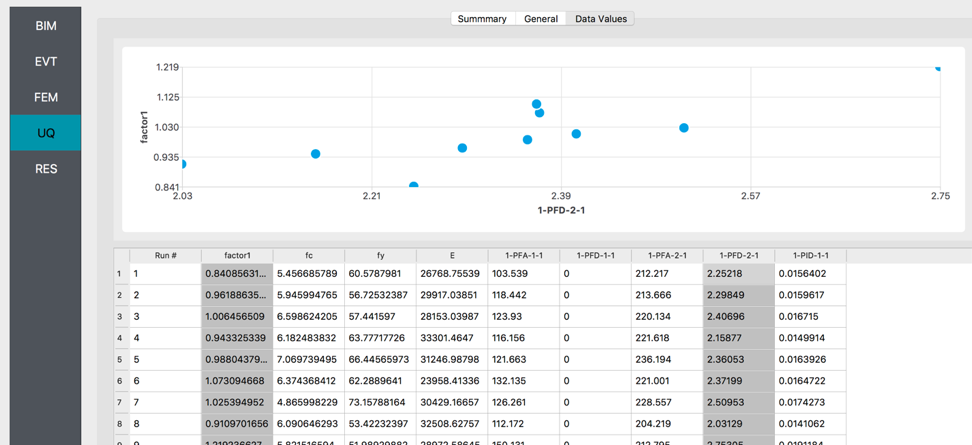
\includegraphics[width=0.8\textwidth]
    {figs/Figure14.png} }
  \caption{UQ Data Values}
  \label{fig:figure14}
\end{figure}


\section{Push Buttons}
There are a number of buttons in the Push Button area of \autoref{fig:figure1}:
\subsection{RUN – to run the simulation of the user’s desktop machine.}
\begin{figure}[!htbp]
  \centering {
    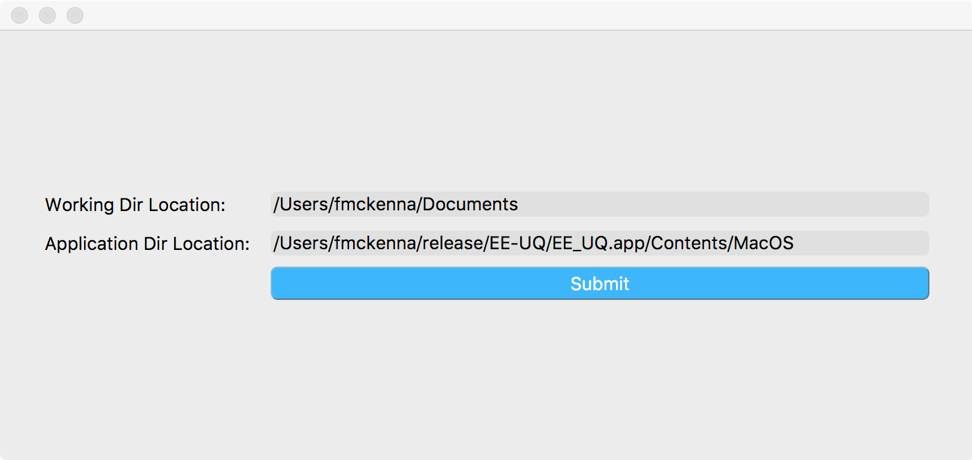
\includegraphics[width=0.8\textwidth]
    {figs/Figure15.png} }
  \caption{Run button}
  \label{fig:figure15}
\end{figure}
The window that pops up is as shown in \autoref{fig:figure15}. There are 2 entries and a push button: 

\begin{itemize}
\item Working Dir Location: specifies where the $EE_UQ$ application can create a “temporary” directory called tmp. SimCenter that the application 
creates when the submit button is pressed. The application creates this directory, copies files to it that the application needs as a result of your 
input (e.g. if you are using OpenSees input script, it will to the tmp. SimCenter directory copy that script, ALL FILES IN THAT DIRECTORY AND ALL FILES IN 
SUBDIRECTORIES OF THAT DIRECTORY GET COPIED SO DON’T PLACE THE SCRIPT IN HOME, DOWNLOADS, DOCUMENTS, ….
\item Application Dir Location: SHOULD NOT BE TOUCHED unless you are introducing your own applications or want to build and modify the 
applications provided with the tool. It is this directory the application tool looks to find the applications to run.
\end{itemize}


Finally, when inputs are finished the user hits submit button to start the backend job. If it runs the window will close and the RES 
panel will pop up on successful run. Do not press the submit button multiple times while waiting for it to close. We cannot guarantee 
what will happen and we did not disable the button in this release.

\subsection{RUN at DesignSafe}
Click this button to process the information, and send to DesignSafe where the job will be run on a supercomputer and results stored in your DesignSafe jobs folder.

\begin{figure}[!htbp]
  \centering {
    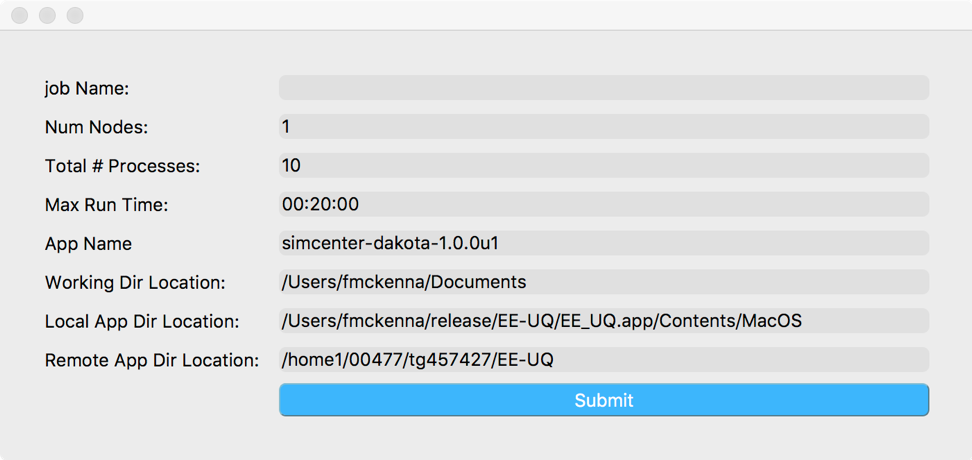
\includegraphics[width=0.8\textwidth]
    {figs/Figure16.png} }
  \caption{Remote button}
  \label{fig:figure16}
\end{figure}

A similar bit longer input panel is brought up:
\begin{itemize}
\item JobName: The name the user can use to identify the job in Get from DesignSafe.
\item NumNodes: The number of compute nodes to use on Stampede2. Using the default App Name the job will run on Stampede2’s KNL Landing (KNL) 
compute nodes. Each node has 68 cores. The actual number of cores the application will use on each of these nodes depends on the total number of 
processes specified. As per the TACC webpage, for MPI tasks it’s best not to specify more than 64-68 processes to run. Depending on the numerical 
computations and amount of memory each uses, so as to avoid page faulting, for large simulations you may wish to use more nodes and less processes.
\item Total Number of Processes: Total number of MPI parallel processes the UQ engine is going to use.
\item Max Wall Time:  HOURS:MIN:SEC be conservative. Your job is killed after the time limit. On Stampede2 you have a max wall time of 24 hours.
\item App Name:   Name of Agave app to run. DO not touch unless you know what you are doing.
\item Working Dir Location: specifies where the $EE_UQ$ application can create a “temporary” directory called tmp. SimCenter that the application 
creates when the submit button is pressed. The application creates this directory, copies files to it that the application needs as a result of your 
input (e.g. if you are using OpenSees input script, it will to the tmp. SimCenter directory copy that script, ALL FILES IN THAT DIRECTORY AND ALL FILES 
IN SUBDIRECTORIES OF THAT DIRECTORY. (SO, DON’T PLACE THE SCRIPT IN HOME, DOWNLOADS, DOCUMENTS, …). That directory is removed when jib has been successfully submitted.
\item Local App Dir Location: SHOULD NOT BE TOUCHED unless you are introducing your own applications or want to build and modify the applications 
provided with the tool. It is this directory the application tool looks to find the applications it needs.
\item Remote App Dir Location: Remote directory on Stampede2 where applications needed by workflow reside. DO not touch unless you know what you are doing.

\end{itemize}


\subsection{GET from DesignSafe}
	Click this button to obtain from DesignSafe your list of jobs and select from that list a job to update status of, download or delete.

\subsection{Exit}
Click this button to exit the application. 


%\chapter{Theory and Implementation}
%\label{chap:theory}
%The following section describes the workings of the tool. If you
intend to use the tool a lot or extend it, it is important that you
read this section.  Some Definitions before we start:
\begin{itemize}
\item Workflow: A sequence of steps involved in moving from a
  beginning state to an ending state.
\item Scientific Workflow Application: An application that automates a
  workflow process through software, with each step in the workflow
  being performed by a separate “scientific” software application.
\item Scientific Workflow System software providing an infrastructure
  for the set-up, scheduling, running, and monitoring of a user
  defined scientific workflow application.
\end{itemize}

The \texttt{\getsoftwarename{}} application is a very limited
scientific workflow system that allows users to create scientific
workflow applications needed for the characterization of the response
of a building subjected to \softwareSwitch{WE-UQ}{wind
  loading}{earthquake ground motions}. It allows the users to then
create and run the workflow application using the data of the users
choosing. The application itself is composed of two parts:

\begin{itemize}
\item Frontend User Interface (UI): This is the application the user
  interacts with to create a building description and
  specify which workflow to run, i.e. given the building, the user
  chooses which applications to use and what data to use for the
  different applications; see \Cref{chap:usage}. As shown in \Cref{fig:figure17}, it 
  creates an input file for the workflow, the BIM, and starts the workflow running.  
\item Backend Application: This is the application that actually
  creates and runs the workflow. It consists of a script that
  processes the output file from the UI to determine the applications
  to run and their data, it invokes these applications using the
  outputs from one application as the input to another. The
  application that is run is a python script, \texttt{\getsoftwarename{}.py}, that can be
  found in the /applications/Workflow/ directory.  The input and
  output from each application is in the form of JavaScript Object
  Notation (\texttt{JSON}) files. \texttt{JSON} is a human readable file format used
  widely for passing data between your front-end browser application
  (Safari, Firefox, Internet Explorer) and backend servers.
\end{itemize}


\begin{figure}[!htbp]
  \centering {
    \includegraphics[width=0.8\textwidth]
    {theory_and_implementation/figures/workflowWithoutUQ.png} }
  \caption{Workflow without uncertainty quantification}
  \label{fig:figure17}
\end{figure}


In the absence of uncertainty, the applications that are invoked by
this script are categorized into certain types of applications, as shown 
in \Cref{fig:figure17}:
\begin{enumerate}
\item createEVENT: given the structure and the user input for hazard
  application, define the loadings for the building, i.e. the
  \softwareSwitch{WE-UQ}{wind loads based on building location, shape,
    and exposure}{ground motions for an earthquake event}. The output
  file is an EVENT file.
\item createSAM: given the building description and event, create a
  finite element model of the building. The output file is a SAM
  (Structural Analysis Model) file.
\item createEDP: given the building, determine what output quantities
  are required. The output file is the EDP (engineering Demand
  Parameters) file.
\item performANA: given the finite element model and the event,
  perform a finite element simulation. The responsibility of the
  performANA is to fill in the values in the EDP files.
\end{enumerate}


The need to characterize the uncertainties in the computed response
complicates this workflow. This is because the uncertainties in the
inputs, random variables and random field variables, may exist for
each application, e.g. Young’s modulus in the building input file,
magnitude of event or event ground motion in createEVENT, finite
element material properties in createSAM, and integration scheme,
damping ratio or convergence tolerance in performANA.

\begin{figure}[!htbp]
  \centering {
    \includegraphics[width=0.8\textwidth]
    {theory_and_implementation/figures/workflowWithUQ.png} }
  \caption{Workflow with uncertainty quantification}
  \label{fig:figure18}
\end{figure}

As a consequence, each application is called with two different sets of
input arguments. The first time the application is invoked with a
“–getRV” input argument. This tells the application to return
information about the random variables inside a “randomVariables”
entry in the p output file generated by the application along with
other needed data, e.g. the event type. The randomVariables is a
\texttt{JSON array} of random variables, each with a field for a name,
a type, a value, and other info that depends on the type, e.g. \\ \\


\begin{lstlisting}
{
  "randomVariables": [
        {
            "distribution": "Normal",
            "mean": 6,
            "name": "fc",
            "stdDev": 0.6,
            "value": "RV.fc",
            "variableClass": "Uncertain"
        },
        {
            "distribution": "Normal",
            "mean": 60,
            "name": "fy",
            "stdDev": 6,
            "value": "RV.fy",
            "variableClass": "Uncertain"
        },
        {
            "distribution": "Normal",
            "mean": 30000,
            "name": "E",
            "stdDev": 3000,
            "value": "RV.E",
            "variableClass": "Uncertain"
        }

}
\end{lstlisting}

It is during the running of the UQ engine that the value field in
these random variables are filled in. Initially as shown, the value
field contains RV.variableName.  This is required must because it is used by
the UQ engine to set the value. When the application is called
again by the UQ engine during it’s running, the application is
called without the “-getRV”. The application finds these value fields
now set to numbers (or strings) in the pFiles. \\

The performUQ application is actually a script that calls 3
applications, as shown below and illustrated in \Cref{fig:uq_sampling}:
\begin{enumerate}
\item PreProcessUQ: to  parse all the pFiles to build the
  list of all random variables.
\item PeformUQ: to invoke the UQ engine, which for the number of
  samples specified will fill in the random variable values, run the
  applications in the workflow with the new files.
\item PostProcessUQ: to process all the output results, filling in
  the EDP’s
\end{enumerate}

\begin{figure}[!htbp]
  \centering {
    \includegraphics[width=0.8\textwidth]
    {theory_and_implementation/figures/uq_sampling.png} }
  \caption{UQ sampling}
  \label{fig:uq_sampling}
\end{figure}

PerformUQ is the computationally expensive part of the simulation.  As
discussed earlier, the user has the option of running locally or
remotely at DesignSafe. When the user selects to run the job remotely,
it is the PerformUQ operation that is run remotely. The operations
peformed in the PreProcessUQ and PostProcessUQ stages are run locally.


%\chapter{Verification and Validation}
%\label{chap:vnv}
%This chapter provides examples of using the \texttt{\getsoftwarename{}} application for uncertainty
quantification of structural analysis models used in earthquake
engineering. Results of each model are verified against results
obtained using other tools.\\

\section{Two-Dimensional Portal Frame subjected to Gravity and Earthquake Loading}
In this example, a simple 2D portal frame model is used to verify the
results of \texttt{EE-UQ}. The model is a linear elastic single-bay,
single-story model of a reinforced concrete portal frame, as shown in
\autoref{fig:figure20}. The analysis of this model considers both
gravity loading and lateral earthquake loading due to the El Centro
earthquake (Borrego Mountain 04/09/68 0230, El Centro ARRAY \#9, 270).
The original model and ground motion used in this example were
obtained from
\href{http://opensees.berkeley.edu/wiki/index.php/OpenSees_Example_1b._Elastic_Portal_Frame}{example 1b} on the \texttt{OpenSees} website, 
and were modified to scale the ground motion record from gravity
units, $g$, to the model units, $in/s^2$. Files for this example are
included with the release of the software and are available in the
Examples folder in a subfolder called \texttt{PortalFrame2D}.

\begin{figure}[!htbp]
  \centering {
    \includegraphics[width=0.8\textwidth]
    {ver_and_val/figures/portalFrame.png} }
  \caption{Two-dimensional portal frame model subjected to gravity and earthquake loading}
  \label{fig:figure20}
\end{figure}

To introduce uncertainty in the model, both mass and young’s modulus
are assumed to be normally distributed random variables with means and
standard deviation values shown in \autoref{tab:uncertainty}. In this
example, the model will be sampled with the Latin Hypercube sampling
method using both \texttt{EE-UQ} and a Python script
(\texttt{PortalFrameSampling.py}) and response statistics from both
analyses are compared.

\begin{table}[hbt!]                       
  \centering
\begin{adjustbox}{max width=\textwidth}            
  \begin{tabular}{lllll}                    
    \toprule          
      Uncertain Parameter & 	Distribution	 &  Mean  &  Standard Deviation \\ \hline
	Nodal Mass, m [kip]	 & Normal & 	5.18	 & 1.0 \\ \hline
	Young’s Modulus, E [ksi] & 	Normal	 & 4227	 & 500.0 \\ \hline
  \end{tabular}
\end{adjustbox}
  \caption{Uncertain parameters defined in the portal frame model}             
  \label{tab:uncertainty}                 
\end{table}

Modeling uncertainty using \texttt{EE-UQ} can be done using the
following steps:
\begin{enumerate}
\item	 Start \texttt{EE-UQ}, click on the simulation tab (SIM) in the left bar to open a building simulation model. Click on choose button in the input script row:

\begin{figure}[!htbp]
  \centering {
    \includegraphics[width=0.8\textwidth]
    {ver_and_val/figures/portalFrameTcl.png} }
  \caption{Choose building model}
  \label{fig:figure21}
\end{figure}

\item	 Choose the model file \texttt{Portal2D-UQ.tcl} from PortalFrame2D example folder.
\begin{figure}[!htbp]
  \centering {
    \includegraphics[width=0.8\textwidth]
    {ver_and_val/figures/tclLocation.png} }
  \caption{Choose tcl file}
  \label{fig:figure22}
\end{figure}


\item	 In the list of Clines Nodes edit box, enter “1, 3”. This indicates to \texttt{EE-UQ} that nodes 1 and 3 are the nodes used to obtain EDP at different floor levels (i.e. base and first floor).
\begin{figure}[!htbp]
  \centering { \includegraphics[width=0.8\textwidth]
    {ver_and_val/figures/cLineNodes.png} } \caption{Select
    nodes} \label{fig:figure23}
\end{figure}

\item Click on the event tab (EVT) in the left bar to open the earthquake event specification tab, select Multiple Existing for loading Type. Click on the add button to add an earthquake event. 
Then click on the choose button to select the event file.
\begin{figure}[!htbp]
  \centering { \includegraphics[width=0.8\textwidth]
    {ver_and_val/figures/workEvtTab.png} }
    \caption{Work on EVT
    tab} \label{fig:figure24}
\end{figure}

\item Choose the event file (\texttt{BM68elc.json}) for El Centro earthquake provided in the portal frame 2D example folder.
\begin{figure}[!htbp]
  \centering {
    \includegraphics[width=0.8\textwidth]
    {ver_and_val/figures/evtFileLocation.png} }
  \caption{Choose event file}
  \label{fig:figure25}
\end{figure}

\item Now select the random variables tab (RVs) from the left bar, change the random variables types to normal and set the mean and standard deviation values of the floor mass and
Young’s modulus.  Notice that \texttt{EE-UQ} has automatically
detected parameters defined in the \texttt{OpenSees} tcl file using the pset
command and defined them as random variables.
\begin{figure}[!htbp]
  \centering {
    \includegraphics[width=0.8\textwidth]
    {ver_and_val/figures/workUqTab.png} }
  \caption{Work on \texttt{UQ} tab}
  \label{fig:figure26}
\end{figure}

\item Now click on run, set the analysis parameters, working directory and applications directory and click submit to run the analysis. 
If everything ran successfully the program will automatically open the
results tab showing the summary of results (\autoref{fig:figure27}).
\begin{figure}[!htbp]
  \centering { \includegraphics[width=0.8\textwidth]
    {ver_and_val/figures/runAnalysis.png} }
    \caption{Pop-up shown when clicking \texttt{Run}}
    \label{fig:figure27}
\end{figure}

\end{enumerate}


\subsection{Verification Script}
A verification script (Listing 1) for propagating the uncertainty was
developed in Python and is included in the example folder.  The script
creates 1000 samples for both the Young’s modulus and mass values
using Latin Hypercube sampling, then modifies the \texttt{OpenSees}
model, runs it and stores the output.  After all the model samples are
processed, the script will compute and output the mean and standard
deviation values of the peak floor acceleration and peak drift.


\begin{python}[caption=Python script for analyzing the portal frame model with uncertain parameters]
import numpy as np
import os
import shutil
import subprocess
from pyDOE import *
from scipy.stats.distributions import norm

#Setting number of samples
nSamples = 1000

#Creating latin hyper cube designs
design = lhs(2, samples=nSamples)

#Sampling Young's Modulus and Mass
ESamples = norm(loc=4227, scale=500.0).ppf(design[:,0])
mSamples = norm(loc=5.18, scale=1.0).ppf(design[:,1])

#Initializing output arrays
PFA = []
PID = []
#Reading OpenSees Model
with open ("Ex1b.Portal2D.EQ.tcl", "r") as portalFrameFile:
    portalFrameModel = portalFrameFile.read()

    #Looping through the samples and creating modified models
    for i in range(nSamples):
        sampleName = str(i+1)
        if(os.path.exists(sampleName) and os.path.isdir(sampleName)):
            shutil.rmtree(sampleName)

        os.mkdir(sampleName)
        shutil.copy('BM68elc.acc', sampleName)

        #Modifying the model using sample E and m values
        with open (sampleName + '/Ex1b.Portal2D.EQ.tcl' , "w+") as modifiedFile:
            modifiedModel = portalFrameModel.replace('pset floorMass 5.18', 'pset floorMass ' + str(mSamples[i]))
            modifiedModel = modifiedModel.replace('pset E 4227', 'pset E ' + str(ESamples[i]))
            modifiedFile.write(modifiedModel)

        #Running OpenSees
        subprocess.Popen("OpenSees Ex1b.Portal2D.EQ.tcl", shell=True, cwd=sampleName).wait()

        #Reading Peak Floor Acceleration
        with open (sampleName + '/PFA.out' , "r") as pfaFile:
            PFA.append(float(pfaFile.readlines()[2]))

        #Reading Peak Floor Acceleration
        with open (sampleName + '/PID.out' , "r") as pidFile:
            PID.append(float(pidFile.readlines()[2]))

        #Cleaning up
        shutil.rmtree(sampleName)

#Printing results
print 'Mean Peak Floor Acceleration: ', np.mean(PFA)
print 'Peak Floor Acceleration Std. Dev: ', np.std(PFA)

print 'Mean Peak Drift: ', np.mean(PID)
print 'Peak Drift Std. Dev.: ', np.std(PID)
\end{python}

\subsection{Verification of Results}
In this section, the results produced for the portal frame
by \texttt{EE-UQ} are verified against the results of running the same
problem using the Python script.  Running the uncertainty
quantification problem on the local computer produces the results
shown in \autoref{fig:figure28} Running the analysis using the
sampling Python script produces the results shown
in \autoref{fig:figure29}.  Both results (Mean and standard deviation
values of EDPs) are compared in \autoref{tab:edp} and are shown to be in good
agreement.

\begin{figure}[!htbp]
  \centering {
    \includegraphics[width=0.8\textwidth]
    {ver_and_val/figures/resultsSummaryTab.png} }
  \caption{Outputs from \texttt{EE-UQ}}
  \label{fig:figure28}
\end{figure}


\begin{figure}[!htbp]
  \centering {
    \includegraphics[width=0.8\textwidth]
    {ver_and_val/figures/pyOutputs.png} }
  \caption{Outputs from PortalFrameSamplying.py script}
  \label{fig:figure29}
\end{figure}

\begin{table}[hbt!]                 
  \centering
\begin{adjustbox}{max width=\textwidth}            
  \begin{tabular}{lllll}                    
    \toprule          
      Engineering Demand Parameter &	 & \texttt{EE-UQ}	& Python Script	 & Percent Difference [\%]  \\ \hline
    
	\multirow{2}{*}{Peak Floor Acceleration [in/$s^2$]} 
	 & Mean &	68.0836	& 67.5448	& 0.80 \\
      & Std. Dev.	& 12.6956	 & 12.5487	& 1.17 \\ \hline
      
      \multirow{2}{*}{Peak Story Drift [x10-3 in]} 
      & Mean &	1.3384 &	1.347 &	1.97 \\
      & Std. Dev.	& 0.3017 &	0.2955	& 2.1	 \\

      \bottomrule      
                            
  \end{tabular}
\end{adjustbox}
  \caption{Engineering demand parameters verification}             
  \label{tab:edp}                 
\end{table}


\softwareSwitch{WE-UQ}{
\section{Power Spectral Density Calculation using Stochastic Wind Model}
The purpose of this analysis is to verify
that \texttt{\getsoftwarename{}} is able to reproduce the correct
power spectral density when using stochastically generated wind speed
time histories. These time histories are generated using a discrete
frequency function and Fast Fourier Transform, as described in
Wittig \& Sinha (1975) \cite{wittig1975simulation}. The calculated
power spectral density matrix for the generated time histories is compared to
an analytical spectral density matrix based on the Kaimal wind spectrum
model \cite{kaimal1972spectral, simiu1996wind} and the Davenport coherence
function \cite{davenport1967dependence}:

\begin{equation}
\bm{S}_{rs} = \sqrt{\bm{S}_{rr}(f) \cdot \bm{S}_{ss}(f)} Coh(f)
\end{equation}

\noindent where $\bm{S}_{rr}$ and $\bm{S}_{ss}$ are power spectral densities
of fluctuating wind at locations $r$ and $s$ respectively; $Coh(f)$ is the
Davenport coherence function; and $f$ is the frequency in Hz. This gives
the two-dimensional, $n$-variate power spectral density matrix $\bm{S}(f)$:

\begin{equation}
   \bm{S}(f) =
      \begin{bmatrix}
         S_{11}(f) & S_{12}(f) & \dots & S_{1n}(f) \\
         S_{21}(f) & S_{12}(f) & \dots & S_{2n}(f) \\
         \vdots & \vdots & \ddots & \vdots \\
         S_{n1}(f) & S_{n2}(f) & \dots & S_{nn}(f) \\         
      \end{bmatrix}
\end{equation}\\

\noindent The power spectral density based on the Kaimal wind spectrum is
defined as:

\begin{equation}
\bm{S}_{rr}(z_{r}, f) = u_{*}^{2} \cdot \frac{200 z_{r}}{\bar{U}(z_{r})} \cdot
              \frac{1}{\left[1 + 50 \frac{f z_{r}}{\bar{U}(z_{r})}\right]^{\frac{5}{3}}}
\end{equation}

\noindent where $\bm{S}_{rr}(f)$ is the power spectral density of the fluctuating
wind at location $z_{r}$ and frequency $f$ in Hz; $\bar{U}(z_{r})$ is
the mean wind speed at location $z_{r}$; and $u_{*}$ is the friction
velocity. The one-sided Davenport coherence function describes the correlation
between fluctuating winds at locations $z_{r}$ and $z_{s}$:

\begin{equation}
Coh(f) = \text{exp}\left[-\frac{C_{z}f\lvert z_{r} -
       z_{s}\rvert}{\frac{1}{2}\left[\bar{U}(z_{r}) + \bar{U}(z_{s})\right]}\right]
\end{equation}\\

\noindent The mean wind velocity at location $z_{r}$ is defined based on exposure conditions
defined in the ASCE 7 standard as follows:

\begin{equation}
\bar{U}(z) = \bar{b} \left(\frac{z}{33}\right)^{\bar{\alpha}}\left(\frac{88}{60}\right)V
\end{equation}

\noindent where $\bar{b}$ and $\bar{\alpha}$ are constants defined in ASCE 7 for
different exposure conditions; $V$ is the 3-second gust wind speed in miles
per hour.

\begin{figure}[!htbp]
  \centering {
    \includegraphics[width=0.8\textwidth]
    {./ver_and_val/figures/S11.pdf} }
  \caption{Comparison between theoretical and simulated auto power
    spectral density at the height of the first floor}
  \label{fig:auto_corr}
\end{figure}

\begin{figure}[!htbp]
  \centering {
    \includegraphics[width=0.8\textwidth]
    {./ver_and_val/figures/S23.pdf} }
  \caption{Comparison between theoretical and simulated cross power
    spectral density between the heights of the second and third floors}
  \label{fig:cross_corr}
\end{figure}

In the validation example, a 3-story structure with exposure category
D is subjected to wind loading with 3-second gust of 30 mph. An
estimate of the power spectral density matrix for the stochastic wind
velocity time history based on this condition was compared to the
power spectral density matrix calculated based on the Kaimal spectrum
with Davenport coherence. \Cref{fig:auto_corr} shows the auto correlation
for the first floor ($S_{11}$) while \Cref{fig:cross_corr} shows the cross
correlation between the second and third floors ($S_{23}$). As can be seen in
these two figures, the two different results show very good agreement
between the theoretical Kaimal values and the estimates based on the
generated stochastic wind velocity time history. Further information
on the implementation of the Wittig \& Sinha (1975) model can be found
in the documentation
for \href{https://github.com/NHERI-SimCenter/smelt}{\texttt{smelt}}\textemdash
a C++ library for stochastically generating time histories for
different types of natural hazards.

}{
\section{Response Spectrum Calculation using Stochastic Ground Motion Model}
The purpose of this analysis is to verify that \texttt{EE-UQ} is able
to reproduce the correct pseudo-acceleration response spectrum when
using synthetic acceleration time histories generated using the
stochastic ground motion model option as the seismic event. The maximum
pseudo-acceleration for a single-degree-of-freedom system with varying
natural frequencies calculated by \texttt{EE-UQ} is compared to the
values predicted by \texttt{smelt} as well as the geometric mean
of the four NGA-West2 ground motion prediction equations (GPMEs)
that account for soil sites. The scenario considered in this verification
example is an event with a Moment Magnitude ($M_W$) of 6.5, closest-to-site
rupture distance ($R_{rupt}$) of 20 \textit{km}, and average shear-wave velocity in the top
30 \textit{m} of soil ($V_{s_{30}}$) equal to 400 \texttt{m/s}.

The single-degree-of-freedom system was input using the MDOF option as
the Building Model Input in \texttt{EE-UQ}. Here, the mass was set to
unity and the damping ratio to 5\%. The story stiffness was modified
to set the natural frequency of the system in order to calculate the
response spectrum. The structural response was calculated for 10
sample synthetic acceleration time histories for each structural
period and compared to those from \texttt{smelt} and the GMPEs, as
shown in \autoref{fig:stochastic_validation}. As can be seen in this
figure, the spectral response calculated by \texttt{EE-UQ} falls
within the mean plus/minus one sigma bounds of the GMPEs and
\texttt{smelt} while tending toward the mean. This produces the
expected result as \texttt{EE-UQ} is calling \texttt{smelt} in the
backend to generate the synthetic motions. The full validation of
\texttt{smelt} in implementing the predictive stochastic model
proposed by Vlachos et al. (2018) \cite{vlachos2018predictive} can be
found in the
\href{https://github.com/shellshocked2003/Stochastic-Loading-Module/blob/master/README.md}{library
  documentation}.

\begin{figure}[!htbp]
  \centering {
    \includegraphics[width=0.8\textwidth]
    {ver_and_val/figures/M65R20V400.pdf} }
  \caption{Response Spectra generated using NGA-West2 GMPEs,
    \texttt{smelt} \& \texttt{EE-UQ} for $M_W = 6.5$, closest-to-site
    distance $R_{rupt} = 20km$, and average shear-wave velocity $V_{s_{30}} =
    400m/s$. The \texttt{smelt} and GMPE spectra show the mean and
    mean plus/minus one logarithmic standard deviation. The GMPE
    spectra are based on the geometric mean of the four NGA-West2
    models that account for site soil conditions. The \texttt{smelt}
    spectra are based on an ensemble of 1000 synthetic ground
    motions. \texttt{EE-UQ} response values are based on the mean
    pseudo-acceleration for 10 synthetic ground motion samples per
    period, $T_n$}
  \label{fig:stochastic_validation}
\end{figure}

}

\section{Site Response Analysis using s$^3$hark}
A 2D free field effective stress analysis is performed by s$^3$hark
and demonstrated here.  The results are verified against FLAC and
Plaxis.  The soil column being analyzed is 6 meters high sitting on a
rock.  The ground water table is at 2 meters below the soil surface.
In the column, there are a total of three soil layers. Each layer is
meshed by elements with a size of 0.25 meter in height.  Basic
properties of soil layers and the rock are shown
in \autoref{fig:s3harkSoilColumn} and \autoref{fig:s3hark5}.  The
first two layers are modeled by PM4Sand and the third layer is modeled
by elastic isotropic material.  (The implementation work of
PM4Sand \cite{boulanger2015pm4sand} is done in University of
Washington by Long Chen and Pedro Arduino.  Chaofeng Wang at UC,
Berkeley contributed to the code optimization for speed improvement. )
The rock layer will be simplified to a \cite{Lysmer:1969} dashpot,
which accounts for the finite rigidity of the underlying elastic
medium.  The parameters of the dashpot are calculated solely based on
rock layer's density and V$_{s30}$.


\begin{figure}[!htbp]
  \centering {
    \includegraphics[width=0.5\textwidth]
    {ver_and_val/figures/s3harkSoilColumn.png} }
  \caption{Soil layers }
  \label{fig:s3harkSoilColumn}
\end{figure}


\begin{figure}[!htbp]
  \centering {
    \includegraphics[width=0.5\textwidth]
    {ver_and_val/figures/s3hark5.png} }
  \caption{Soil layers }
  \label{fig:s3hark5}
\end{figure}


The detailed properties of the material in each soil layer are shown in \autoref{fig:s3hark6}.

\begin{figure}[!htbp]
  \centering 
  \subfloat[Layer 1]{
    \includegraphics[width=0.4\textwidth]
    {ver_and_val/figures/layer1.png}}
  \subfloat[Layer 2]{
    \includegraphics[width=0.39\textwidth]
    {ver_and_val/figures/layer2.png}}
    
    \subfloat[Layer 3]{
    \includegraphics[width=0.4\textwidth]
    {ver_and_val/figures/layer3.png}}
  \caption{Detail soil properties and material model parameters}
  \label{fig:s3hark6}
\end{figure}

For the verification and validation purposes, s$^3$hark's results are compared with FLAC an PLAXIS, as shown in \autoref{fig:s3hark7}. 
All three programs generally produce very similar response with
different levels of differences shown in PHA, maximum shear strain, CSR, maximum pore pressure ratio. 
The differences come from multiple sources, such as numerical discretization methods, solvers, etc.
For example, FLAC tends to produce higher dilation pulses in liquefied layer. 
This is possibly due to a combination of different reasons, e.g.,
interpolation of data from integration points at different
locations, numerical methods for integration, formulations for
solid fluid coupling, etc.
(Chaofeng Wang at UC, Berkeley, Long Chen and Andrew Makdisi at University of Washington,  
Gregor Vilhar at PLAXIS, BV contributed to the verification of PM4Sand in s$^3$hark. )

\begin{figure}[!htbp]
  \centering {
    \includegraphics[width=0.7\textwidth]
    {ver_and_val/figures/N10T3_RSN766_ProfileCompare.jpg} }
  \caption{Soil layers }
  \label{fig:s3hark7}
\end{figure}



%\chapter{Source Code}
%\label{chap:SourceCode}
%This source code for the tool is released under the 2-clause BSD
License, commonly called the FreeBSD license.  It is available for
download from the
tool's \href{https://github.com/NHERI-SimCenter/EE-UQ}{GitHub
repository}


%\chapter{User Training}
%\label{chap:training}
%User Training consists of an online video available from the tool
webpage that demonstrates tool use. The tool will be presented in user
workshops hosted by the SimCenter.


%\chapter{Requirements}
%\label{chap:requirements}
%This chapter outlines the general features of the \texttt{\getsoftwarename{}} application. We show when the features were introduced and what features and when you can expect to see in the future. This provides a roadmap of where this application has come from and where it is headed. The future features are highly dependent on user feedback. You are highly encouraged to contact us to discuss any new features you would like to see in the application.\\



%\chapter{Troubleshooting}
%\label{chap:troubleshooting}
%The \texttt{\getsoftwarename{}} can be a complicated tool and it will not always run. Causes of failure include incorrect set up, non-functioing or poorly functioining websites, and of course user error. To discover the errors it is useful to understand how the UI and the backend work when the user submits to run a job. A number of things occur when the Submit button is clicked: 

\begin{enumerate}
\item The UI creates a folder in the workging dir location specified called tmp.SimCenter and in that folder creates another folder called templatedir.
\item The UI then iterates through all the widgets chosen and these widgets place all needed files for the computation into the templatedir directory.
\item A python script is run in this templatedir directory that creates the input file for the UQ Engine. For example, using Dakota the input file dakota.in is created and placed in tmp.SimCenter folder.
\item The UQ engine is then started and runs using the dakota.in input file.
\item As the UQ engine runs, it creates folders in tmp.SimCenter, one folder for each deterministic run.
\item When completed the UQ engine leaves the results files in the tmp.SimCenter folder.
\item The results files are then processed by the UI and presented to the user in the RES tab.
\end{enumerate}

The following is a list of things that we have observed to go wrong when the UI informs the user of a failure and steps the user can take to fix the problem:  

\begin{enumerate}
\item \textbf{Could not create working dir}: The user does not have permission to create the tmp.SimCenter folder in working dir location. Change the Working Dir location in the window that pops up.
\item \textbf{No Script File}: The user has changed the Applications dir location, or the applications folder that accompanies the installation has been modified. Either set the correct dir location or re-install the tool.
\item \textbf{ERROR: Dakota failed to finish}: This can occur for a number of reasons. Go to the tmp.SimCenter folder and have a look for the dakota.err file.
\begin{enumerate}
\item \textbf{No dakota.err file and no dakota.in file}: the python script in templatdir failed to create the necessary files. Have a look at the workflow log file in templatedir folder to see what the error is as it could indicate an error in your input.
\item \textbf{No dakota.err and dakota.in exists}: Dakota failed to run. Check install of Dakota.
\item \textbf{dakota.err file exists}: Open the file and see what the error is.  For example if it says \textbf{Error: at least one variable must be specified.} This means no random variables have been specified. So whether you have only one  deterministic event or you have not specified any random variables in the EDP.
\item \textbf{dakota.err file exists but is empty}: This means that Dakota ran but there was a problem with the simulation. Go to one of the workdir locations. There is a file workflow driver that can be run. Run it and see what the errors are.
\item \textbf{You ran at DesignSafe and no dakota.out files come back}: Go to your data depot older at DesignSafe using the browser. Go to archive/jobs and use the job number shown in table that pops up when you ask to get the job from DesignSafe. look at the .err file in that directory for a clues to as what went wrong.
\item \textbf{No results and you used the Site Response to create the event}. You must run a simulated event in the Site Response Widget before you can submit a job to run.
\end{enumerate}
\end{enumerate}

If still having trouble, you can always join the \texttt{\getsoftwarename{}} slack channel and look for similar issues or post a new one.



\nocite{*}

% \appendix
% \chapter{More Monticello Candidates}

\pagestyle{plain}
{
  \renewcommand{\thispagestyle}[1]{}	
  \printbibliography           
}

\end{document}
